% generated from JIRA project LVV
% using template at /usr/share/miniconda/envs/docsteady-env/lib/python3.7/site-packages/docsteady/templates/tpr.latex.jinja2.
% using docsteady version 2.2.9
% Please do not edit -- update information in Jira instead
\documentclass[DM,lsstdraft,STR,toc]{lsstdoc}
\usepackage{geometry}
\usepackage{longtable,booktabs}
\usepackage{enumitem}
\usepackage{arydshln}
\usepackage{attachfile}
\usepackage{array}
\usepackage{dashrule}

\newcolumntype{L}[1]{>{\raggedright\let\newline\\\arraybackslash\hspace{0pt}}p{#1}}

\input meta.tex

\newcommand{\attachmentsUrl}{https://github.com/\gitorg/\lsstDocType-\lsstDocNum/blob/\gitref/attachments}
\providecommand{\tightlist}{
  \setlength{\itemsep}{0pt}\setlength{\parskip}{0pt}}

\setcounter{tocdepth}{4}

\begin{document}

\def\milestoneName{Data Management Acceptance Test Campaign 1}
\def\milestoneId{}
\def\product{Acceptance}

\setDocCompact{true}

\title{LVV-P99: Data Management Acceptance Test Campaign 1 Test Plan and Report}
\setDocRef{\lsstDocType-\lsstDocNum}
\date{ 2022-08-23 }
\author{ Jeffrey Carlin }

% Most recent last
\setDocChangeRecord{
\addtohist{}{2022-07-12}{First draft}{Jeff Carlin}
\addtohist{1.0}{2023-01-17}{Test campaign LVV-P99 completed and results approved. DM-32340}{Jeff Carlin}
}

\setDocCurator{Jeff Carlin}
\setDocUpstreamLocation{\url{https://github.com/lsst-dm/\lsstDocType-\lsstDocNum}}
\setDocUpstreamVersion{34628ca}
%\setDocUpstreamVersion{\vcsRevision}



\setDocAbstract{
This is the test plan and report for
\textbf{ Data Management Acceptance Test Campaign 1},
an LSST milestone pertaining to the Data Management Subsystem.\\
This document is based on content automatically extracted from the Jira test database on \docDate.
The most recent change to the document repository was on \vcsDate.
}


\maketitle

\section{Introduction}
\label{sect:intro}


\subsection{Objectives}
\label{sect:objectives}

 The primary goal of this DM acceptance test campaign will be to verify
priority 1a DMSR (\citeds{LSE-61}) requirements that have not been verified as
part of prior testing and milestones. Any priority 1b, 2, or 3
requirements that have been completed will also be verified.



\subsection{System Overview}
\label{sect:systemoverview}

 This test campaign is intended to verify that the DM system satisfies at
least half of the priority 1a requirements outlined in the Data
Management System Requirements (DMSR;
\href{https://lse-61.lsst.io/}{LSE-61} ), ensuring that we are
progressing toward readiness for the installation and operation of
ComCam. Additional DMSR requirements will be verified in later
Acceptance Test Campaigns.\\[2\baselineskip]\textbf{Applicable
Documents:}\\
\citeds{LSE-61}: Data Management System (DMS) Requirements\\
\citeds{LDM-503} Data Management Test Plan\\
\citeds{LDM-639}: Data Management Acceptance Test
Specification\\[2\baselineskip]Tests in this campaign will use data
products and artifacts from Data Preview 0.2, which consists of DESC
Data Challenge 2 (DC2) simulated data reprocessed using the LSST Science
Pipelines. Additional on-sky data from auxTel imaging campaigns will be
used when appropriate.


\subsection{Document Overview}
\label{sect:docoverview}

This document was generated from Jira, obtaining the relevant information from the
\href{https://jira.lsstcorp.org/secure/Tests.jspa\#/testPlan/LVV-P99}{LVV-P99}
~Jira Test Plan and related Test Cycles (
\href{https://jira.lsstcorp.org/secure/Tests.jspa\#/testCycle/LVV-C208}{LVV-C208}
).

Section \ref{sect:intro} provides an overview of the test campaign, the system under test (\product{}),
the applicable documentation, and explains how this document is organized.
Section \ref{sect:testplan} provides additional information about the test plan, like for example the configuration
used for this test or related documentation.
Section \ref{sect:personnel} describes the necessary roles and lists the individuals assigned to them.

Section \ref{sect:overview} provides a summary of the test results, including an overview in Table \ref{table:summary},
an overall assessment statement and suggestions for possible improvements.
Section \ref{sect:detailedtestresults} provides detailed results for each step in each test case.

The current status of test plan \href{https://jira.lsstcorp.org/secure/Tests.jspa\#/testPlan/LVV-P99}{LVV-P99} in Jira is \textbf{ Draft }.

\subsection{References}
\label{sect:references}
\renewcommand{\refname}{}
\bibliography{lsst,refs,books,refs_ads,local}


\newpage
\section{Test Plan Details}
\label{sect:testplan}


\subsection{Data Collection}

  Observing is not required for this test campaign.

\subsection{Verification Environment}
\label{sect:hwconf}
  Most testing will be performed using the Rubin Science Platform (RSP),
hosted at the IDF, with auxTel-related tests using the development
cluster at the USDF. In particular, we will use version X\_XXXX\_XX of
the Pipelines.




\subsection{Related Documentation}


No additional documentation provided.


\subsection{PMCS Activity}

Primavera milestones related to the test campaign:
\begin{itemize}
\item None
\end{itemize}


\newpage
\section{Personnel}
\label{sect:personnel}

The personnel involved in the test campaign is shown in the following table.

{\small
\begin{longtable}{p{3cm}p{3cm}p{3cm}p{6cm}}
\hline
\multicolumn{2}{r}{T. Plan \href{https://jira.lsstcorp.org/secure/Tests.jspa\#/testPlan/LVV-P99}{LVV-P99} owner:} &
\multicolumn{2}{l}{\textbf{ Jeffrey Carlin } }\\\hline
\multicolumn{2}{r}{T. Cycle \href{https://jira.lsstcorp.org/secure/Tests.jspa\#/testCycle/LVV-C208}{LVV-C208} owner:} &
\multicolumn{2}{l}{\textbf{
Jeffrey Carlin }
} \\\hline
\textbf{Test Cases} & \textbf{Assigned to} & \textbf{Executed by} & \textbf{Additional Test Personnel} \\ \hline
\href{https://jira.lsstcorp.org/secure/Tests.jspa#/testCase/LVV-T32}{LVV-T32}
& {\small Kian-Tat Lim } & {\small  } &
\begin{minipage}[]{6cm}
\smallskip
{\small  }
\medskip
\end{minipage}
\\ \hline
\href{https://jira.lsstcorp.org/secure/Tests.jspa#/testCase/LVV-T374}{LVV-T374}
& {\small John Swinbank } & {\small  } &
\begin{minipage}[]{6cm}
\smallskip
{\small  }
\medskip
\end{minipage}
\\ \hline
\href{https://jira.lsstcorp.org/secure/Tests.jspa#/testCase/LVV-T362}{LVV-T362}
& {\small John Swinbank } & {\small  } &
\begin{minipage}[]{6cm}
\smallskip
{\small  }
\medskip
\end{minipage}
\\ \hline
\href{https://jira.lsstcorp.org/secure/Tests.jspa#/testCase/LVV-T368}{LVV-T368}
& {\small John Swinbank } & {\small  } &
\begin{minipage}[]{6cm}
\smallskip
{\small  }
\medskip
\end{minipage}
\\ \hline
\href{https://jira.lsstcorp.org/secure/Tests.jspa#/testCase/LVV-T1756}{LVV-T1756}
& {\small Jeffrey Carlin } & {\small  } &
\begin{minipage}[]{6cm}
\smallskip
{\small  }
\medskip
\end{minipage}
\\ \hline
\href{https://jira.lsstcorp.org/secure/Tests.jspa#/testCase/LVV-T124}{LVV-T124}
& {\small Simon Krughoff } & {\small  } &
\begin{minipage}[]{6cm}
\smallskip
{\small  }
\medskip
\end{minipage}
\\ \hline
\href{https://jira.lsstcorp.org/secure/Tests.jspa#/testCase/LVV-T199}{LVV-T199}
& {\small Robert Gruendl [X] } & {\small  } &
\begin{minipage}[]{6cm}
\smallskip
{\small  }
\medskip
\end{minipage}
\\ \hline
\href{https://jira.lsstcorp.org/secure/Tests.jspa#/testCase/LVV-T83}{LVV-T83}
& {\small Robert Lupton } & {\small  } &
\begin{minipage}[]{6cm}
\smallskip
{\small  }
\medskip
\end{minipage}
\\ \hline
\href{https://jira.lsstcorp.org/secure/Tests.jspa#/testCase/LVV-T190}{LVV-T190}
& {\small Robert Gruendl [X] } & {\small  } &
\begin{minipage}[]{6cm}
\smallskip
{\small  }
\medskip
\end{minipage}
\\ \hline
\href{https://jira.lsstcorp.org/secure/Tests.jspa#/testCase/LVV-T77}{LVV-T77}
& {\small Jim Bosch } & {\small  } &
\begin{minipage}[]{6cm}
\smallskip
{\small  }
\medskip
\end{minipage}
\\ \hline
\href{https://jira.lsstcorp.org/secure/Tests.jspa#/testCase/LVV-T84}{LVV-T84}
& {\small Robert Lupton } & {\small  } &
\begin{minipage}[]{6cm}
\smallskip
{\small  }
\medskip
\end{minipage}
\\ \hline
\href{https://jira.lsstcorp.org/secure/Tests.jspa#/testCase/LVV-T88}{LVV-T88}
& {\small Robert Lupton } & {\small  } &
\begin{minipage}[]{6cm}
\smallskip
{\small  }
\medskip
\end{minipage}
\\ \hline
\href{https://jira.lsstcorp.org/secure/Tests.jspa#/testCase/LVV-T115}{LVV-T115}
& {\small Kian-Tat Lim } & {\small  } &
\begin{minipage}[]{6cm}
\smallskip
{\small  }
\medskip
\end{minipage}
\\ \hline
\href{https://jira.lsstcorp.org/secure/Tests.jspa#/testCase/LVV-T151}{LVV-T151}
& {\small Colin Slater } & {\small  } &
\begin{minipage}[]{6cm}
\smallskip
{\small  }
\medskip
\end{minipage}
\\ \hline
\href{https://jira.lsstcorp.org/secure/Tests.jspa#/testCase/LVV-T1232}{LVV-T1232}
& {\small Colin Slater } & {\small  } &
\begin{minipage}[]{6cm}
\smallskip
{\small  }
\medskip
\end{minipage}
\\ \hline
\href{https://jira.lsstcorp.org/secure/Tests.jspa#/testCase/LVV-T149}{LVV-T149}
& {\small Colin Slater } & {\small  } &
\begin{minipage}[]{6cm}
\smallskip
{\small  }
\medskip
\end{minipage}
\\ \hline
\href{https://jira.lsstcorp.org/secure/Tests.jspa#/testCase/LVV-T72}{LVV-T72}
& {\small Jim Bosch } & {\small  } &
\begin{minipage}[]{6cm}
\smallskip
{\small  }
\medskip
\end{minipage}
\\ \hline
\href{https://jira.lsstcorp.org/secure/Tests.jspa#/testCase/LVV-T85}{LVV-T85}
& {\small Robert Lupton } & {\small  } &
\begin{minipage}[]{6cm}
\smallskip
{\small  }
\medskip
\end{minipage}
\\ \hline
\href{https://jira.lsstcorp.org/secure/Tests.jspa#/testCase/LVV-T90}{LVV-T90}
& {\small Robert Lupton } & {\small  } &
\begin{minipage}[]{6cm}
\smallskip
{\small  }
\medskip
\end{minipage}
\\ \hline
\href{https://jira.lsstcorp.org/secure/Tests.jspa#/testCase/LVV-T137}{LVV-T137}
& {\small Colin Slater } & {\small  } &
\begin{minipage}[]{6cm}
\smallskip
{\small  }
\medskip
\end{minipage}
\\ \hline
\href{https://jira.lsstcorp.org/secure/Tests.jspa#/testCase/LVV-T55}{LVV-T55}
& {\small Eric Bellm } & {\small  } &
\begin{minipage}[]{6cm}
\smallskip
{\small  }
\medskip
\end{minipage}
\\ \hline
\href{https://jira.lsstcorp.org/secure/Tests.jspa#/testCase/LVV-T146}{LVV-T146}
& {\small Robert Gruendl [X] } & {\small  } &
\begin{minipage}[]{6cm}
\smallskip
{\small  }
\medskip
\end{minipage}
\\ \hline
\href{https://jira.lsstcorp.org/secure/Tests.jspa#/testCase/LVV-T66}{LVV-T66}
& {\small Jim Bosch } & {\small  } &
\begin{minipage}[]{6cm}
\smallskip
{\small  }
\medskip
\end{minipage}
\\ \hline
\href{https://jira.lsstcorp.org/secure/Tests.jspa#/testCase/LVV-T91}{LVV-T91}
& {\small Robert Lupton } & {\small  } &
\begin{minipage}[]{6cm}
\smallskip
{\small  }
\medskip
\end{minipage}
\\ \hline
\href{https://jira.lsstcorp.org/secure/Tests.jspa#/testCase/LVV-T126}{LVV-T126}
& {\small Eric Bellm } & {\small  } &
\begin{minipage}[]{6cm}
\smallskip
{\small  }
\medskip
\end{minipage}
\\ \hline
\href{https://jira.lsstcorp.org/secure/Tests.jspa#/testCase/LVV-T1946}{LVV-T1946}
& {\small Jeffrey Carlin } & {\small Jeffrey Carlin } &
\begin{minipage}[]{6cm}
\smallskip
{\small  }
\medskip
\end{minipage}
\\ \hline
\href{https://jira.lsstcorp.org/secure/Tests.jspa#/testCase/LVV-T1947}{LVV-T1947}
& {\small Jeffrey Carlin } & {\small Jeffrey Carlin } &
\begin{minipage}[]{6cm}
\smallskip
{\small  }
\medskip
\end{minipage}
\\ \hline
\href{https://jira.lsstcorp.org/secure/Tests.jspa#/testCase/LVV-T28}{LVV-T28}
& {\small Colin Slater } & {\small Jeffrey Carlin } &
\begin{minipage}[]{6cm}
\smallskip
{\small  }
\medskip
\end{minipage}
\\ \hline
\href{https://jira.lsstcorp.org/secure/Tests.jspa#/testCase/LVV-T78}{LVV-T78}
& {\small Kian-Tat Lim } & {\small  } &
\begin{minipage}[]{6cm}
\smallskip
{\small  }
\medskip
\end{minipage}
\\ \hline
\href{https://jira.lsstcorp.org/secure/Tests.jspa#/testCase/LVV-T42}{LVV-T42}
& {\small Jim Bosch } & {\small  } &
\begin{minipage}[]{6cm}
\smallskip
{\small  }
\medskip
\end{minipage}
\\ \hline
\href{https://jira.lsstcorp.org/secure/Tests.jspa#/testCase/LVV-T38}{LVV-T38}
& {\small Eric Bellm } & {\small  } &
\begin{minipage}[]{6cm}
\smallskip
{\small  }
\medskip
\end{minipage}
\\ \hline
\href{https://jira.lsstcorp.org/secure/Tests.jspa#/testCase/LVV-T141}{LVV-T141}
& {\small Robert Gruendl [X] } & {\small  } &
\begin{minipage}[]{6cm}
\smallskip
{\small  }
\medskip
\end{minipage}
\\ \hline
\href{https://jira.lsstcorp.org/secure/Tests.jspa#/testCase/LVV-T140}{LVV-T140}
& {\small Robert Gruendl [X] } & {\small  } &
\begin{minipage}[]{6cm}
\smallskip
{\small  }
\medskip
\end{minipage}
\\ \hline
\href{https://jira.lsstcorp.org/secure/Tests.jspa#/testCase/LVV-T129}{LVV-T129}
& {\small Robert Lupton } & {\small  } &
\begin{minipage}[]{6cm}
\smallskip
{\small  }
\medskip
\end{minipage}
\\ \hline
\href{https://jira.lsstcorp.org/secure/Tests.jspa#/testCase/LVV-T127}{LVV-T127}
& {\small Robert Lupton } & {\small Jeffrey Carlin } &
\begin{minipage}[]{6cm}
\smallskip
{\small  }
\medskip
\end{minipage}
\\ \hline
\href{https://jira.lsstcorp.org/secure/Tests.jspa#/testCase/LVV-T131}{LVV-T131}
& {\small Gregory Dubois-Felsmann } & {\small  } &
\begin{minipage}[]{6cm}
\smallskip
{\small  }
\medskip
\end{minipage}
\\ \hline
\href{https://jira.lsstcorp.org/secure/Tests.jspa#/testCase/LVV-T79}{LVV-T79}
& {\small Jim Bosch } & {\small  } &
\begin{minipage}[]{6cm}
\smallskip
{\small  }
\medskip
\end{minipage}
\\ \hline
\href{https://jira.lsstcorp.org/secure/Tests.jspa#/testCase/LVV-T1830}{LVV-T1830}
& {\small Jeffrey Carlin } & {\small  } &
\begin{minipage}[]{6cm}
\smallskip
{\small  }
\medskip
\end{minipage}
\\ \hline
\href{https://jira.lsstcorp.org/secure/Tests.jspa#/testCase/LVV-T98}{LVV-T98}
& {\small Kian-Tat Lim } & {\small  } &
\begin{minipage}[]{6cm}
\smallskip
{\small  }
\medskip
\end{minipage}
\\ \hline
\href{https://jira.lsstcorp.org/secure/Tests.jspa#/testCase/LVV-T145}{LVV-T145}
& {\small Robert Lupton } & {\small  } &
\begin{minipage}[]{6cm}
\smallskip
{\small  }
\medskip
\end{minipage}
\\ \hline
\href{https://jira.lsstcorp.org/secure/Tests.jspa#/testCase/LVV-T144}{LVV-T144}
& {\small Kian-Tat Lim } & {\small  } &
\begin{minipage}[]{6cm}
\smallskip
{\small  }
\medskip
\end{minipage}
\\ \hline
\href{https://jira.lsstcorp.org/secure/Tests.jspa#/testCase/LVV-T74}{LVV-T74}
& {\small Eric Bellm } & {\small Jeffrey Carlin } &
\begin{minipage}[]{6cm}
\smallskip
{\small  }
\medskip
\end{minipage}
\\ \hline
\href{https://jira.lsstcorp.org/secure/Tests.jspa#/testCase/LVV-T97}{LVV-T97}
& {\small Kian-Tat Lim } & {\small  } &
\begin{minipage}[]{6cm}
\smallskip
{\small  }
\medskip
\end{minipage}
\\ \hline
\href{https://jira.lsstcorp.org/secure/Tests.jspa#/testCase/LVV-T1529}{LVV-T1529}
& {\small Jeffrey Carlin } & {\small  } &
\begin{minipage}[]{6cm}
\smallskip
{\small  }
\medskip
\end{minipage}
\\ \hline
\href{https://jira.lsstcorp.org/secure/Tests.jspa#/testCase/LVV-T1527}{LVV-T1527}
& {\small Jeffrey Carlin } & {\small  } &
\begin{minipage}[]{6cm}
\smallskip
{\small  }
\medskip
\end{minipage}
\\ \hline
\href{https://jira.lsstcorp.org/secure/Tests.jspa#/testCase/LVV-T1758}{LVV-T1758}
& {\small Jeffrey Carlin } & {\small  } &
\begin{minipage}[]{6cm}
\smallskip
{\small  }
\medskip
\end{minipage}
\\ \hline
\href{https://jira.lsstcorp.org/secure/Tests.jspa#/testCase/LVV-T1528}{LVV-T1528}
& {\small Jeffrey Carlin } & {\small  } &
\begin{minipage}[]{6cm}
\smallskip
{\small  }
\medskip
\end{minipage}
\\ \hline
\end{longtable}
}

\newpage

\section{Test Campaign Overview}
\label{sect:overview}

\subsection{Summary}
\label{sect:summarytable}

{\small
\begin{longtable}{p{2cm}cp{2.3cm}p{8.6cm}p{2.3cm}}
\toprule
\multicolumn{2}{r}{ T. Plan \href{https://jira.lsstcorp.org/secure/Tests.jspa\#/testPlan/LVV-P99}{LVV-P99}:} &
\multicolumn{2}{p{10.9cm}}{\textbf{ Data Management Acceptance Test Campaign 1 }} & Draft \\\hline
\multicolumn{2}{r}{ T. Cycle \href{https://jira.lsstcorp.org/secure/Tests.jspa\#/testCycle/LVV-C208}{LVV-C208}:} &
\multicolumn{2}{p{10.9cm}}{\textbf{ Data Management Acceptance Test Campaign 1 }} & In Progress \\\hline
\textbf{Test Cases} &  \textbf{Ver.} & \textbf{Status} & \textbf{Comment} & \textbf{Issues} \\\toprule
\href{https://jira.lsstcorp.org/secure/Tests.jspa#/testCase/LVV-T32}{LVV-T32}
&  1
& Not Executed &
\begin{minipage}[]{9cm}
\smallskip

\medskip
\end{minipage}
&   \\\hline
\href{https://jira.lsstcorp.org/secure/Tests.jspa#/testCase/LVV-T374}{LVV-T374}
&  1
& Not Executed &
\begin{minipage}[]{9cm}
\smallskip

\medskip
\end{minipage}
&   \\\hline
\href{https://jira.lsstcorp.org/secure/Tests.jspa#/testCase/LVV-T362}{LVV-T362}
&  1
& Not Executed &
\begin{minipage}[]{9cm}
\smallskip

\medskip
\end{minipage}
&   \\\hline
\href{https://jira.lsstcorp.org/secure/Tests.jspa#/testCase/LVV-T368}{LVV-T368}
&  2
& Not Executed &
\begin{minipage}[]{9cm}
\smallskip

\medskip
\end{minipage}
&   \\\hline
\href{https://jira.lsstcorp.org/secure/Tests.jspa#/testCase/LVV-T1756}{LVV-T1756}
&  1
& Not Executed &
\begin{minipage}[]{9cm}
\smallskip

\medskip
\end{minipage}
&   \\\hline
\href{https://jira.lsstcorp.org/secure/Tests.jspa#/testCase/LVV-T124}{LVV-T124}
&  1
& Not Executed &
\begin{minipage}[]{9cm}
\smallskip

\medskip
\end{minipage}
&   \\\hline
\href{https://jira.lsstcorp.org/secure/Tests.jspa#/testCase/LVV-T199}{LVV-T199}
&  1
& Not Executed &
\begin{minipage}[]{9cm}
\smallskip

\medskip
\end{minipage}
&   \\\hline
\href{https://jira.lsstcorp.org/secure/Tests.jspa#/testCase/LVV-T83}{LVV-T83}
&  1
& Not Executed &
\begin{minipage}[]{9cm}
\smallskip

\medskip
\end{minipage}
&   \\\hline
\href{https://jira.lsstcorp.org/secure/Tests.jspa#/testCase/LVV-T190}{LVV-T190}
&  1
& Not Executed &
\begin{minipage}[]{9cm}
\smallskip

\medskip
\end{minipage}
&   \\\hline
\href{https://jira.lsstcorp.org/secure/Tests.jspa#/testCase/LVV-T77}{LVV-T77}
&  1
& Not Executed &
\begin{minipage}[]{9cm}
\smallskip

\medskip
\end{minipage}
&   \\\hline
\href{https://jira.lsstcorp.org/secure/Tests.jspa#/testCase/LVV-T84}{LVV-T84}
&  1
& Not Executed &
\begin{minipage}[]{9cm}
\smallskip

\medskip
\end{minipage}
&   \\\hline
\href{https://jira.lsstcorp.org/secure/Tests.jspa#/testCase/LVV-T88}{LVV-T88}
&  1
& Not Executed &
\begin{minipage}[]{9cm}
\smallskip

\medskip
\end{minipage}
&   \\\hline
\href{https://jira.lsstcorp.org/secure/Tests.jspa#/testCase/LVV-T115}{LVV-T115}
&  1
& Not Executed &
\begin{minipage}[]{9cm}
\smallskip

\medskip
\end{minipage}
&   \\\hline
\href{https://jira.lsstcorp.org/secure/Tests.jspa#/testCase/LVV-T151}{LVV-T151}
&  1
& Not Executed &
\begin{minipage}[]{9cm}
\smallskip

\medskip
\end{minipage}
&   \\\hline
\href{https://jira.lsstcorp.org/secure/Tests.jspa#/testCase/LVV-T1232}{LVV-T1232}
&  1
& Not Executed &
\begin{minipage}[]{9cm}
\smallskip

\medskip
\end{minipage}
&   \\\hline
\href{https://jira.lsstcorp.org/secure/Tests.jspa#/testCase/LVV-T149}{LVV-T149}
&  1
& Not Executed &
\begin{minipage}[]{9cm}
\smallskip

\medskip
\end{minipage}
&   \\\hline
\href{https://jira.lsstcorp.org/secure/Tests.jspa#/testCase/LVV-T72}{LVV-T72}
&  1
& Not Executed &
\begin{minipage}[]{9cm}
\smallskip

\medskip
\end{minipage}
&   \\\hline
\href{https://jira.lsstcorp.org/secure/Tests.jspa#/testCase/LVV-T85}{LVV-T85}
&  1
& Not Executed &
\begin{minipage}[]{9cm}
\smallskip

\medskip
\end{minipage}
&   \\\hline
\href{https://jira.lsstcorp.org/secure/Tests.jspa#/testCase/LVV-T90}{LVV-T90}
&  1
& Not Executed &
\begin{minipage}[]{9cm}
\smallskip

\medskip
\end{minipage}
&   \\\hline
\href{https://jira.lsstcorp.org/secure/Tests.jspa#/testCase/LVV-T137}{LVV-T137}
&  1
& Not Executed &
\begin{minipage}[]{9cm}
\smallskip

\medskip
\end{minipage}
&   \\\hline
\href{https://jira.lsstcorp.org/secure/Tests.jspa#/testCase/LVV-T55}{LVV-T55}
&  1
& Not Executed &
\begin{minipage}[]{9cm}
\smallskip

\medskip
\end{minipage}
&   \\\hline
\href{https://jira.lsstcorp.org/secure/Tests.jspa#/testCase/LVV-T146}{LVV-T146}
&  1
& Not Executed &
\begin{minipage}[]{9cm}
\smallskip

\medskip
\end{minipage}
&   \\\hline
\href{https://jira.lsstcorp.org/secure/Tests.jspa#/testCase/LVV-T66}{LVV-T66}
&  1
& Not Executed &
\begin{minipage}[]{9cm}
\smallskip

\medskip
\end{minipage}
&   \\\hline
\href{https://jira.lsstcorp.org/secure/Tests.jspa#/testCase/LVV-T91}{LVV-T91}
&  1
& Not Executed &
\begin{minipage}[]{9cm}
\smallskip

\medskip
\end{minipage}
&   \\\hline
\href{https://jira.lsstcorp.org/secure/Tests.jspa#/testCase/LVV-T126}{LVV-T126}
&  1
& Not Executed &
\begin{minipage}[]{9cm}
\smallskip

\medskip
\end{minipage}
&   \\\hline
\href{https://jira.lsstcorp.org/secure/Tests.jspa#/testCase/LVV-T1946}{LVV-T1946}
&  1
& Pass &
\begin{minipage}[]{9cm}
\smallskip
Executed at the IDF using Science Pipelines version
w\_2022\_32.\\[2\baselineskip]This test case can be executed by running
the script test\_LVV-T1946.py, which is available in the test report
github repository's ``scripts/'' directory.\\[2\baselineskip]Note that
in this test we only checked source catalogs that are persisted in
butler repositories. Catalogs in other forms (e.g., parquet tables, or
tables in the Qserv database) will be confirmed separately.
\medskip
\end{minipage}
&   \\\hline
\href{https://jira.lsstcorp.org/secure/Tests.jspa#/testCase/LVV-T1947}{LVV-T1947}
&  1
& Pass &
\begin{minipage}[]{9cm}
\smallskip
Executed at the IDF using Science Pipelines version
w\_2022\_32.\\[2\baselineskip]This test case can be executed by running
the script test\_LVV-T1947.py, which is available in the test report
github repository's ``scripts/'' directory.\\[2\baselineskip]Note that
in this test we only checked source catalogs that are persisted in
butler repositories. Catalogs in other forms (e.g., parquet tables, or
tables in the Qserv database) will be confirmed separately.
\medskip
\end{minipage}
&   \\\hline
\href{https://jira.lsstcorp.org/secure/Tests.jspa#/testCase/LVV-T28}{LVV-T28}
&  1
& Pass &
\begin{minipage}[]{9cm}
\smallskip
Executed at the IDF using Science Pipelines version
w\_2022\_32.\\[2\baselineskip]This test case can be executed by running
the script test\_LVV-T28.py, which is available in the test report
github repository's ``scripts/'' directory.\\[2\baselineskip]Note that
in this test we only checked source catalogs that are persisted in
butler repositories. Catalogs in other forms (e.g., parquet tables, or
tables in the Qserv database) will be confirmed separately.
\medskip
\end{minipage}
&   \\\hline
\href{https://jira.lsstcorp.org/secure/Tests.jspa#/testCase/LVV-T78}{LVV-T78}
&  1
& Not Executed &
\begin{minipage}[]{9cm}
\smallskip

\medskip
\end{minipage}
&   \\\hline
\href{https://jira.lsstcorp.org/secure/Tests.jspa#/testCase/LVV-T42}{LVV-T42}
&  1
& Not Executed &
\begin{minipage}[]{9cm}
\smallskip

\medskip
\end{minipage}
&   \\\hline
\href{https://jira.lsstcorp.org/secure/Tests.jspa#/testCase/LVV-T38}{LVV-T38}
&  1
& Not Executed &
\begin{minipage}[]{9cm}
\smallskip

\medskip
\end{minipage}
&   \\\hline
\href{https://jira.lsstcorp.org/secure/Tests.jspa#/testCase/LVV-T141}{LVV-T141}
&  1
& Not Executed &
\begin{minipage}[]{9cm}
\smallskip

\medskip
\end{minipage}
&   \\\hline
\href{https://jira.lsstcorp.org/secure/Tests.jspa#/testCase/LVV-T140}{LVV-T140}
&  1
& Not Executed &
\begin{minipage}[]{9cm}
\smallskip

\medskip
\end{minipage}
&   \\\hline
\href{https://jira.lsstcorp.org/secure/Tests.jspa#/testCase/LVV-T129}{LVV-T129}
&  1
& Not Executed &
\begin{minipage}[]{9cm}
\smallskip

\medskip
\end{minipage}
&   \\\hline
\href{https://jira.lsstcorp.org/secure/Tests.jspa#/testCase/LVV-T127}{LVV-T127}
&  1
& Pass &
\begin{minipage}[]{9cm}
\smallskip

\medskip
\end{minipage}
&   \\\hline
\href{https://jira.lsstcorp.org/secure/Tests.jspa#/testCase/LVV-T131}{LVV-T131}
&  1
& Not Executed &
\begin{minipage}[]{9cm}
\smallskip

\medskip
\end{minipage}
&   \\\hline
\href{https://jira.lsstcorp.org/secure/Tests.jspa#/testCase/LVV-T79}{LVV-T79}
&  1
& Not Executed &
\begin{minipage}[]{9cm}
\smallskip

\medskip
\end{minipage}
&   \\\hline
\href{https://jira.lsstcorp.org/secure/Tests.jspa#/testCase/LVV-T1830}{LVV-T1830}
&  1
& Not Executed &
\begin{minipage}[]{9cm}
\smallskip

\medskip
\end{minipage}
&   \\\hline
\href{https://jira.lsstcorp.org/secure/Tests.jspa#/testCase/LVV-T98}{LVV-T98}
&  1
& Not Executed &
\begin{minipage}[]{9cm}
\smallskip

\medskip
\end{minipage}
&   \\\hline
\href{https://jira.lsstcorp.org/secure/Tests.jspa#/testCase/LVV-T145}{LVV-T145}
&  1
& Not Executed &
\begin{minipage}[]{9cm}
\smallskip

\medskip
\end{minipage}
&   \\\hline
\href{https://jira.lsstcorp.org/secure/Tests.jspa#/testCase/LVV-T144}{LVV-T144}
&  1
& Not Executed &
\begin{minipage}[]{9cm}
\smallskip

\medskip
\end{minipage}
&   \\\hline
\href{https://jira.lsstcorp.org/secure/Tests.jspa#/testCase/LVV-T74}{LVV-T74}
&  1
& Pass &
\begin{minipage}[]{9cm}
\smallskip
See attached artifact notebook ``test\_LVV-T74.ipynb'' for details.
\medskip
\end{minipage}
&   \\\hline
\href{https://jira.lsstcorp.org/secure/Tests.jspa#/testCase/LVV-T97}{LVV-T97}
&  1
& Not Executed &
\begin{minipage}[]{9cm}
\smallskip

\medskip
\end{minipage}
&   \\\hline
\href{https://jira.lsstcorp.org/secure/Tests.jspa#/testCase/LVV-T1529}{LVV-T1529}
&  1
& Not Executed &
\begin{minipage}[]{9cm}
\smallskip

\medskip
\end{minipage}
&   \\\hline
\href{https://jira.lsstcorp.org/secure/Tests.jspa#/testCase/LVV-T1527}{LVV-T1527}
&  1
& Not Executed &
\begin{minipage}[]{9cm}
\smallskip

\medskip
\end{minipage}
&   \\\hline
\href{https://jira.lsstcorp.org/secure/Tests.jspa#/testCase/LVV-T1758}{LVV-T1758}
&  1
& Not Executed &
\begin{minipage}[]{9cm}
\smallskip

\medskip
\end{minipage}
&   \\\hline
\href{https://jira.lsstcorp.org/secure/Tests.jspa#/testCase/LVV-T1528}{LVV-T1528}
&  1
& Not Executed &
\begin{minipage}[]{9cm}
\smallskip

\medskip
\end{minipage}
&   \\\hline
\caption{Test Campaign Summary}
\label{table:summary}
\end{longtable}
}

\subsection{Overall Assessment}
\label{sect:overallassessment}

Not yet available.

\subsection{Recommended Improvements}
\label{sect:recommendations}

Not yet available.

\newpage
\section{Detailed Test Results}
\label{sect:detailedtestresults}

\subsection{Test Cycle LVV-C208 }

Open test cycle {\it \href{https://jira.lsstcorp.org/secure/Tests.jspa#/testrun/LVV-C208}{Data Management Acceptance Test Campaign 1}} in Jira.

Test Cycle name: Data Management Acceptance Test Campaign 1\\
Status: In Progress

This test cycle verifies a subset of
\href{https://lse-61.lsst.io/}{DMSR} (\citeds{LSE-61}) requirements in order to
verify their completion and readiness for LSST Operations (i.e., that
the requirements laid out in \citeds{LSE-61} have been met by the DM Systems).
Testing will use data products and artifacts from Data Preview 0.2
reprocessing of DESC DC2 data.

\subsubsection{Software Version/Baseline}
Using Science Pipelines version w\_2022\_32 on the interim data facility
(IDF) at data.lsst.cloud.

\subsubsection{Configuration}
Not provided.

\subsubsection{Test Cases in LVV-C208 Test Cycle}

\paragraph{ LVV-T32 - Verify implementation of Raw Image Assembly }\mbox{}\\

Version \textbf{1}.
Open  \href{https://jira.lsstcorp.org/secure/Tests.jspa#/testCase/LVV-T32}{\textit{ LVV-T32 } }
test case in Jira.

Verify that the raw exposure data from all readout channels in a sensor
can be assembled into a single image, and that all required/relevant
metadata are associated with the image data.~

\textbf{ Preconditions}:\\


Execution status: {\bf Not Executed }

Final comment:\\


Detailed steps results:

\begin{tabular}{p{2cm}p{14cm}}
\toprule
Step 1 & Step Execution Status: \textbf{ Not Executed } \\ \hline
\end{tabular}
 Description \\
{\footnotesize
Ingest data from the L1 Camera Test Stand DAQ.

}
\hdashrule[0.5ex]{\textwidth}{1pt}{3mm}
  Expected Result \\
{\footnotesize

}
\hdashrule[0.5ex]{\textwidth}{1pt}{3mm}
  Actual Result \\
{\footnotesize

}
\begin{tabular}{p{2cm}p{14cm}}
\toprule
Step 2 & Step Execution Status: \textbf{ Not Executed } \\ \hline
\end{tabular}
 Description \\
{\footnotesize
Simulate all different modes of data gathering.

}
\hdashrule[0.5ex]{\textwidth}{1pt}{3mm}
  Expected Result \\
{\footnotesize

}
\hdashrule[0.5ex]{\textwidth}{1pt}{3mm}
  Actual Result \\
{\footnotesize

}
\begin{tabular}{p{2cm}p{14cm}}
\toprule
Step 3 & Step Execution Status: \textbf{ Not Executed } \\ \hline
\end{tabular}
 Description \\
{\footnotesize
Verify that a raw image is constructed in correct format.

}
\hdashrule[0.5ex]{\textwidth}{1pt}{3mm}
  Expected Result \\
{\footnotesize
A single raw image combining data from all readout channels for a given
sensor.~

}
\hdashrule[0.5ex]{\textwidth}{1pt}{3mm}
  Actual Result \\
{\footnotesize

}
\begin{tabular}{p{2cm}p{14cm}}
\toprule
Step 4 & Step Execution Status: \textbf{ Not Executed } \\ \hline
\end{tabular}
 Description \\
{\footnotesize
Verify that a raw image is constructed with correct metadata.

}
\hdashrule[0.5ex]{\textwidth}{1pt}{3mm}
  Expected Result \\
{\footnotesize
Image header or ancillary table contains the required metadata about the
observing context in which data were gathered.

}
\hdashrule[0.5ex]{\textwidth}{1pt}{3mm}
  Actual Result \\
{\footnotesize

}

\paragraph{ LVV-T374 - Ingesting Camera test data }\mbox{}\\

Version \textbf{1}.
Open  \href{https://jira.lsstcorp.org/secure/Tests.jspa#/testCase/LVV-T374}{\textit{ LVV-T374 } }
test case in Jira.

This test will check:

\begin{itemize}
\tightlist
\item
  That raw Camera test data is available on a filesystem in the LSST
  Data Facility;
\item
  That raw Camera test data can be ingested and made available through
  the Data Management I/O abstraction (the ``Data Butler'').
\end{itemize}

\textbf{ Preconditions}:\\
Appropriate raw data from Camera test systems must be available on a
filesystem within the LSST Data Facility. This test data is assumed to
include visit 258334666 (hereafter referred to as \$VISIT\_ID) from RTM
(Raft Tower Module) 007 for the purposes of this test, but other,
equivalent, may be substituted.\\[2\baselineskip]At time of writing,
suitable data may be found on the GPFS filesystem at
/project/bootcamp/data/LCA-11021\_RTM-007/7086/fe55\_raft\_acq/v0/44981.
In future, as data transport procedures to the Data Facility become more
streamlined and formalised, this data may be moved elsewhere or made
available through some other system. Throughout the test script, we use
the string ``\$INPUT\_DATA\_DIR'' as an alias for
``/project/bootcamp/data/LCA-11021\_RTM-007/7086/fe55\_raft\_acq/v0/44981'',
or wherever this data has been moved to.\\[2\baselineskip]

Execution status: {\bf Not Executed }

Final comment:\\


Detailed steps results:

\begin{tabular}{p{2cm}p{14cm}}
\toprule
Step 1 & Step Execution Status: \textbf{ Not Executed } \\ \hline
\end{tabular}
 Description \\
{\footnotesize
Connect to the Notebook Aspect of the Science Platform following the
instructions at https://nb.lsst.io/. Log in, and ``spawn'' a new machine
with image ``Weekly 2018\_45`` and size ``large''.

}
\hdashrule[0.5ex]{\textwidth}{1pt}{3mm}
  Expected Result \\
{\footnotesize
The JupyterLab environment appears.

}
\hdashrule[0.5ex]{\textwidth}{1pt}{3mm}
  Actual Result \\
{\footnotesize

}
\begin{tabular}{p{2cm}p{14cm}}
\toprule
Step 2 & Step Execution Status: \textbf{ Not Executed } \\ \hline
\end{tabular}
 Description \\
{\footnotesize
Create a terminal session. Use it to set up the LSST tools, then
download and build version 5c12b06e6 of
obs\_lsst:\\[2\baselineskip]\hspace*{0.333em} ~\$ source
/opt/lsst/software/stack/loadLSST.bash\\
\hspace*{0.333em} ~\$ setup lsst\_distrib\\
\hspace*{0.333em} ~\$ git clone https://github.com/lsst/obs\_lsst.git\\
\hspace*{0.333em} ~\$ cd obs\_lsst\\
\hspace*{0.333em} ~\$ git checkout 5c12b06e6\\
\hspace*{0.333em} ~\$ setup -k -r .\\
\hspace*{0.333em} ~\$ scons

}
\hdashrule[0.5ex]{\textwidth}{1pt}{3mm}
  Expected Result \\
{\footnotesize
No errors are seen during execution of the provided commands.

}
\hdashrule[0.5ex]{\textwidth}{1pt}{3mm}
  Actual Result \\
{\footnotesize

}
\begin{tabular}{p{2cm}p{14cm}}
\toprule
Step 3 & Step Execution Status: \textbf{ Not Executed } \\ \hline
\end{tabular}
 Description \\
{\footnotesize
Ingest RTM-007 test data by executing the following
commands:\\[2\baselineskip]\hspace*{0.333em}
~OUTPUT\_REPO\_DIR=\$OUTPUT\_DATA\_DIR\\
\hspace*{0.333em} ~INPUT\_DATA\_DIR=\$INPUT\_DATA\_DIR\\
\hspace*{0.333em} ~mkdir -p \$OUTPUT\_REPO\_DIR\\
\hspace*{0.333em} ~echo ``lsst.obs.lsst.ts8.Ts8Mapper'' \textgreater{}
\$OUTPUT\_REPO\_DIR/\_mapper\\
\hspace*{0.333em} ~ingestImages.py \$OUTPUT\_REPO\_DIR
\$INPUT\_DATA\_DIR/*/*.fits\\
\hspace*{0.333em} ~constructBias.py \$OUTPUT\_REPO\_DIR --rerun calibs
--id imageType=BIAS --batch-type smp --cores 4\\
\hspace*{0.333em} ~ingestCalibs.py \$OUTPUT\_REPO\_DIR --calibType bias
\$OUTPUT\_REPO\_DIR/rerun/calibs/bias/*/*.fits --validity 9999 --output
\$OUTPUT\_REPO\_DIR/CALIB
--mode=link\\[2\baselineskip]Where:\\[2\baselineskip]\hspace*{0.333em}
~\$OUTPUT\_DATA\_DIR is some location on shared storage to which the
user has write permission;\\
\hspace*{0.333em} ~\$INPUT\_DATA\_DIR is defined in the test case
description.

}
\hdashrule[0.5ex]{\textwidth}{1pt}{3mm}
  Expected Result \\
{\footnotesize
Many status messages are logged to screen, and the command exits with
status 0.

}
\hdashrule[0.5ex]{\textwidth}{1pt}{3mm}
  Actual Result \\
{\footnotesize

}
\begin{tabular}{p{2cm}p{14cm}}
\toprule
Step 4 & Step Execution Status: \textbf{ Not Executed } \\ \hline
\end{tabular}
 Description \\
{\footnotesize
Demonstrate that raw and bias data for visit \$VISIT\_ID have been made
available in the repository. Load a Python interpreter (run ``python'')
and execute the following:\\[2\baselineskip]\hspace*{0.333em} ~from
lsst.daf.persistence import Butler\\
\hspace*{0.333em} ~visit\_id = \$VISIT\_ID\\
\hspace*{0.333em} ~b = Butler(\$OUTPUT\_DATA\_DIR)\\
\hspace*{0.333em} ~b.get(``raw'', visit=visit\_id, detector=2)\\
\hspace*{0.333em} ~b.get(``bias'', visit=visit\_id, detector=2)

}
\hdashrule[0.5ex]{\textwidth}{1pt}{3mm}
  Expected Result \\
{\footnotesize
Each call to b.get() returns an instance of an ExposureF object.
Warnings about lack of dark-time or WCS information may be ignored.

}
\hdashrule[0.5ex]{\textwidth}{1pt}{3mm}
  Actual Result \\
{\footnotesize

}

\paragraph{ LVV-T362 - Installation of the LSST Science Pipelines Payloads }\mbox{}\\

Version \textbf{1}.
Open  \href{https://jira.lsstcorp.org/secure/Tests.jspa#/testCase/LVV-T362}{\textit{ LVV-T362 } }
test case in Jira.

This test will check that:

\begin{itemize}
\tightlist
\item
  The Alert Production Pipeline payload is available for installation
  from documented channels;
\item
  The Data Release Production Pipeline payload is available for
  installation from documented channels;
\item
  The Calibration Products Production Pipeline payload is available for
  installation from documented channels;
\item
  These payloads can be installed on systems at the LSST Data Facility
  following available documentation;
\item
  The installed pipeline payloads are capable of successfully executing
  basic integration tests.
\end{itemize}

Note that this test assumes packaging of the Science Pipelines software,
in which all the above payloads are represented by a single
``meta-package'', lsst\_distrib.

\textbf{ Preconditions}:\\


Execution status: {\bf Not Executed }

Final comment:\\


Detailed steps results:

\begin{tabular}{p{2cm}p{14cm}}
\toprule
Step 1 & Step Execution Status: \textbf{ Not Executed } \\ \hline
\end{tabular}
 Description \\
{\footnotesize
The LSST Science Pipelines, described by the lsst\_distrib meta-package,
should be installed following the documentation available at
https://pipelines.lsst.io/. The suggested Conda environment will be used
to ensure that a supported execution environment is available.

}
\hdashrule[0.5ex]{\textwidth}{1pt}{3mm}
  Expected Result \\
{\footnotesize
Detailed output will depend on the installation method chosen, but will
confirm the successful installation of the Science Pipelines.

}
\hdashrule[0.5ex]{\textwidth}{1pt}{3mm}
  Actual Result \\
{\footnotesize

}
\begin{tabular}{p{2cm}p{14cm}}
\toprule
Step 2 & Step Execution Status: \textbf{ Not Executed } \\ \hline
\end{tabular}
 Description \\
{\footnotesize
The lsst\_distrib top-level metapackage will be enabled. Assuming that
the software has been installed at
\$\{LSST\_DIR\}:\\[2\baselineskip]\hspace*{0.333em} ~ ~ ~source
\$\{LSST\_DIR\}/loadLSST.bash\\
\hspace*{0.333em} ~ ~ ~setup lsst\_distrib

}
\hdashrule[0.5ex]{\textwidth}{1pt}{3mm}
  Expected Result \\
{\footnotesize
Nothing is printed. The command\\[2\baselineskip]\hspace*{0.333em} ~eups
list -s lsst\_distrib\\[2\baselineskip]may be used to confirm that the
correct version of the codebase has been installed.

}
\hdashrule[0.5ex]{\textwidth}{1pt}{3mm}
  Actual Result \\
{\footnotesize

}
\begin{tabular}{p{2cm}p{14cm}}
\toprule
Step 3 & Step Execution Status: \textbf{ Not Executed } \\ \hline
\end{tabular}
 Description \\
{\footnotesize
The ``LSST Stack Demo'' package will be downloaded onto the test system
from https://github.com/lsst/pipelines\_check/releases. The version
corresponding to to the version of the Science Pipelines under test
should be chosen.

}
\hdashrule[0.5ex]{\textwidth}{1pt}{3mm}
  Expected Result \\
{\footnotesize
Depends on the tool selected by the user for downloading.

}
\hdashrule[0.5ex]{\textwidth}{1pt}{3mm}
  Actual Result \\
{\footnotesize

}
\begin{tabular}{p{2cm}p{14cm}}
\toprule
Step 4 & Step Execution Status: \textbf{ Not Executed } \\ \hline
\end{tabular}
 Description \\
{\footnotesize
The stack demo package is uncompressed into a directory \$\{DEMO\_DIR\}.

}
\hdashrule[0.5ex]{\textwidth}{1pt}{3mm}
  Expected Result \\
{\footnotesize
Depends on options given to the tar command. Should confirm the
availability of the stack demo source.

}
\hdashrule[0.5ex]{\textwidth}{1pt}{3mm}
  Actual Result \\
{\footnotesize

}
\begin{tabular}{p{2cm}p{14cm}}
\toprule
Step 5 & Step Execution Status: \textbf{ Not Executed } \\ \hline
\end{tabular}
 Description \\
{\footnotesize
The demo package will be executed by following the instructions in its
README file.~

}
\hdashrule[0.5ex]{\textwidth}{1pt}{3mm}
  Expected Result \\
{\footnotesize
Successful execution will result in the string ``Ok'' being returned.

}
\hdashrule[0.5ex]{\textwidth}{1pt}{3mm}
  Actual Result \\
{\footnotesize

}

\paragraph{ LVV-T368 - Loading and processing Camera test data }\mbox{}\\

Version \textbf{2}.
Open  \href{https://jira.lsstcorp.org/secure/Tests.jspa#/testCase/LVV-T368}{\textit{ LVV-T368 } }
test case in Jira.

This test will check:

\begin{itemize}
\tightlist
\item
  That Camera test data is available for processing in the LSST Data
  Facility, and accessible through the LSST Science Platform;
\item
  That the Data Management I/O abstraction (the ``Data Butler'') can
  load that data into the Science Platform environment;
\item
  That Data Management algorithmic ``tasks'' can be executed to process
  that data;
\item
  That results can be displayed in the Firefly display tool.
\end{itemize}

\textbf{ Preconditions}:\\
Appropriate data --- to include a ``raw'' and a ``bias'' exposure ---
from the Camera test systems must be available in a Butler data
repository on a filesystem accessible to the Notebook Aspect of the
Science Platform.\\[2\baselineskip]For the purposes of the following
discussion, we assume that:\\[2\baselineskip]

\begin{itemize}
\tightlist
\item
  Visit 258334666 from RTM (Raft Tower Module) 007 will be used;
\item
  The data is available in a repository at
  /project/bootcamp/repo\_RTM-007/ on the Data Facility GPFS filesystem
\end{itemize}

In the test script, we refer to ``258334666'' as ``\$VISIT\_ID'' and
``/project/bootcamp/repo\_RTM-007/'' as ``\$REPOSITORY\_PATH''; other
data may be substituted as appropriate.

Execution status: {\bf Not Executed }

Final comment:\\


Detailed steps results:

\begin{tabular}{p{2cm}p{14cm}}
\toprule
Step 1 & Step Execution Status: \textbf{ Not Executed } \\ \hline
\end{tabular}
 Description \\
{\footnotesize
Connect to the Notebook Aspect of the Science Platform following the
instructions at https://nb.lsst.io/. Log in, and ``spawn'' a new machine
with image ``Weekly 2018\_45`` and size ``small''.

}
\hdashrule[0.5ex]{\textwidth}{1pt}{3mm}
  Expected Result \\
{\footnotesize
The JupyterLab environment appears.

}
\hdashrule[0.5ex]{\textwidth}{1pt}{3mm}
  Actual Result \\
{\footnotesize

}
\begin{tabular}{p{2cm}p{14cm}}
\toprule
Step 2 & Step Execution Status: \textbf{ Not Executed } \\ \hline
\end{tabular}
 Description \\
{\footnotesize
Create a terminal session. Use it to set up the LSST tools, then
download and build version 5c12b06e6 of
obs\_lsst:\\[2\baselineskip]\hspace*{0.333em} ~\$ source
/opt/lsst/software/stack/loadLSST.bash\\
\hspace*{0.333em} ~\$ setup lsst\_distrib\\
\hspace*{0.333em} ~\$ git clone https://github.com/lsst/obs\_lsst.git\\
\hspace*{0.333em} ~\$ cd obs\_lsst\\
\hspace*{0.333em} ~\$ git checkout 5c12b06e6\\
\hspace*{0.333em} ~\$ setup -k -r .\\
\hspace*{0.333em} ~\$ scons\\[2\baselineskip]Arrange for obs\_lsst to
automatically be added to the environment when starting a new
notebook:\\[2\baselineskip]\hspace*{0.333em} ~\$ echo ``setup -j -r
\textasciitilde{}/obs\_lsst'' \textgreater{}\textgreater{}
\textasciitilde{}/notebooks/.user\_setups\\[2\baselineskip]Exit the
terminal.

}
\hdashrule[0.5ex]{\textwidth}{1pt}{3mm}
  Expected Result \\
{\footnotesize
No errors are seen during execution of the provided commands.

}
\hdashrule[0.5ex]{\textwidth}{1pt}{3mm}
  Actual Result \\
{\footnotesize

}
\begin{tabular}{p{2cm}p{14cm}}
\toprule
Step 3 & Step Execution Status: \textbf{ Not Executed } \\ \hline
\end{tabular}
 Description \\
{\footnotesize
Create a new ``LSST'' notebook.\\[2\baselineskip]Import the standard
libraries required for the rest of this
test:\\[2\baselineskip]\hspace*{0.333em} ~import os\\
\hspace*{0.333em} ~import lsst.afw.display as afwDisplay\\
\hspace*{0.333em} ~from lsst.daf.persistence import Butler\\
\hspace*{0.333em} ~from lsst.ip.isr import IsrTask\\
\hspace*{0.333em} ~from firefly\_client import FireflyClient\\
\hspace*{0.333em} ~from IPython.display import
IFrame\\[2\baselineskip]and execute the cell.

}
\hdashrule[0.5ex]{\textwidth}{1pt}{3mm}
  Expected Result \\
{\footnotesize
Nothing is printed.

}
\hdashrule[0.5ex]{\textwidth}{1pt}{3mm}
  Actual Result \\
{\footnotesize

}
\begin{tabular}{p{2cm}p{14cm}}
\toprule
Step 4 & Step Execution Status: \textbf{ Not Executed } \\ \hline
\end{tabular}
 Description \\
{\footnotesize
Create a Data Butler client, and use it to retrieve the data which will
be used for this test.\\[2\baselineskip]\hspace*{0.333em} ~butler =
Butler(\$REPOSITORY\_PATH)\\
\hspace*{0.333em} ~raw = butler.get(``raw'', visit=\$VISIT\_ID,
detector=2)\\
\hspace*{0.333em} ~bias = butler.get(``bias'', visit=\$VISIT\_ID,
detector=2)

}
\hdashrule[0.5ex]{\textwidth}{1pt}{3mm}
  Expected Result \\
{\footnotesize
Nothing is printed.

}
\hdashrule[0.5ex]{\textwidth}{1pt}{3mm}
  Actual Result \\
{\footnotesize

}
\begin{tabular}{p{2cm}p{14cm}}
\toprule
Step 5 & Step Execution Status: \textbf{ Not Executed } \\ \hline
\end{tabular}
 Description \\
{\footnotesize
Initialize the Firefly display
system:\\[2\baselineskip]\hspace*{0.333em} ~my\_channel =
`\{\}\_test\_channel'.format(os.environ{[}'USER'{]})\\
\hspace*{0.333em} ~server = `https://lsst-lspdev.ncsa.illinois.edu'\\
\hspace*{0.333em}
~ff='\{\}/firefly/slate.html?\_\_wsch=\{\}'.format(server,
my\_channel)\\
\hspace*{0.333em} ~IFrame(ff,800,600)\\
\hspace*{0.333em} ~afwDisplay.setDefaultBackend('firefly')\\
\hspace*{0.333em} ~afw\_display = afwDisplay.getDisplay(frame=1,\\
\hspace*{0.333em} ~ ~ ~ ~ ~ ~ ~ ~ ~ ~ ~ ~ ~ ~ ~ ~ ~ ~
~name=my\_channel)\\[2\baselineskip]Click on the link provided after
executing the above.

}
\hdashrule[0.5ex]{\textwidth}{1pt}{3mm}
  Expected Result \\
{\footnotesize
A Firefly window is shown.

}
\hdashrule[0.5ex]{\textwidth}{1pt}{3mm}
  Actual Result \\
{\footnotesize

}
\begin{tabular}{p{2cm}p{14cm}}
\toprule
Step 6 & Step Execution Status: \textbf{ Not Executed } \\ \hline
\end{tabular}
 Description \\
{\footnotesize
Display the raw image data in the Firefly
window:\\[2\baselineskip]\hspace*{0.333em} afw\_display.mtv(raw)

}
\hdashrule[0.5ex]{\textwidth}{1pt}{3mm}
  Expected Result \\
{\footnotesize
Raw image data is displayed.

}
\hdashrule[0.5ex]{\textwidth}{1pt}{3mm}
  Actual Result \\
{\footnotesize

}
\begin{tabular}{p{2cm}p{14cm}}
\toprule
Step 7 & Step Execution Status: \textbf{ Not Executed } \\ \hline
\end{tabular}
 Description \\
{\footnotesize
Configure and run an Instrument Signature Removal (ISR) task on the raw
data. Most corrections are disabled for simplicity. but the bias frame
is applied.\\
\hspace*{0.333em}

\begin{verbatim}
   isr_config = IsrTask.ConfigClass()
   isr_config.doDark=False
   isr_config.doFlat=False
   isr_config.doFringe=False
   isr_config.doDefect=False
   isr_config.doAddDistortionModel=False
   isr_config.doLinearize=False
   isr = IsrTask(config=isr_config)
   result = isr.run(raw, bias=bias)
\end{verbatim}

}
\hdashrule[0.5ex]{\textwidth}{1pt}{3mm}
  Expected Result \\
{\footnotesize
Nothing is printed.

}
\hdashrule[0.5ex]{\textwidth}{1pt}{3mm}
  Actual Result \\
{\footnotesize

}
\begin{tabular}{p{2cm}p{14cm}}
\toprule
Step 8 & Step Execution Status: \textbf{ Not Executed } \\ \hline
\end{tabular}
 Description \\
{\footnotesize
Display the corrected image data in the Firefly
window:\\[2\baselineskip]\hspace*{0.333em}
~afw\_display.mtv(result.exposure)

}
\hdashrule[0.5ex]{\textwidth}{1pt}{3mm}
  Expected Result \\
{\footnotesize
Processed (trimmed, bias-subtracted) image data is displayed.

}
\hdashrule[0.5ex]{\textwidth}{1pt}{3mm}
  Actual Result \\
{\footnotesize

}

\paragraph{ LVV-T1756 - Verify calculation of photometric repeatability in uzy filters }\mbox{}\\

Version \textbf{1}.
Open  \href{https://jira.lsstcorp.org/secure/Tests.jspa#/testCase/LVV-T1756}{\textit{ LVV-T1756 } }
test case in Jira.

Verify that the DM system has provided the code to calculate the RMS
photometric repeatability of bright non-saturated unresolved point
sources in the u, z, and y filters, and assess whether it meets the
requirement that it shall be less than \textbf{PA1uzy = 7.5
millimagnitudes}.

\textbf{ Preconditions}:\\


Execution status: {\bf Not Executed }

Final comment:\\


Detailed steps results:

\begin{tabular}{p{2cm}p{14cm}}
\toprule
Step 1 & Step Execution Status: \textbf{ Not Executed } \\ \hline
\end{tabular}
 Description \\
{\footnotesize
Identify a dataset containing at least one field in each of the u, z,
and y filters with multiple overlapping visits.

}
\hdashrule[0.5ex]{\textwidth}{1pt}{3mm}
  Expected Result \\
{\footnotesize
A dataset that has been ingested into a Butler repository.

}
\hdashrule[0.5ex]{\textwidth}{1pt}{3mm}
  Actual Result \\
{\footnotesize

}
\begin{tabular}{p{2cm}p{14cm}}
\toprule
Step 2 & Step Execution Status: \textbf{ Not Executed } \\ \hline
\end{tabular}
 Description \\
{\footnotesize
Execute `faro` on a repository containing processed data. Identify the
path to the data, which we will call `DATA/path', then execute something
similar to the following (with paths, datasets, and flags replaced or
additionally specified as needed):

}
\hdashrule[0.5ex]{\textwidth}{1pt}{3mm}
  Example Code \\
{\footnotesize
pipetask --long-log run -j 2 -b DATA/path/butler.yaml
--register-dataset-types -p \$FARO\_DIR/pipelines/metrics\_pipeline.yaml
-d ``band in ('g', `r', `i') AND tract=9813 AND skymap='hsc\_rings\_v1'
AND instrument='HSC''' --output u/username/faro\_metrics -i
HSC/runs/RC2/w\_2021\_06 2\textgreater{}\&1 \textbar{} tee
w06\_2021\_tract9813\_faro.txt

}
\hdashrule[0.5ex]{\textwidth}{1pt}{3mm}
  Expected Result \\
{\footnotesize
The output collection (in this case, ``u/username/faro\_metrics'')
containing metric measurements and any associated extras and metadata is
available via the butler.

}
\hdashrule[0.5ex]{\textwidth}{1pt}{3mm}
  Actual Result \\
{\footnotesize

}
\begin{tabular}{p{2cm}p{14cm}}
\toprule
Step 3 & Step Execution Status: \textbf{ Not Executed } \\ \hline
\end{tabular}
 Description \\
{\footnotesize
Confirm that the metric PA1uzy has been calculated, and that its values
are reasonable.

}
\hdashrule[0.5ex]{\textwidth}{1pt}{3mm}
  Expected Result \\
{\footnotesize
A JSON file (and/or a report generated from that JSON file)
demonstrating that PA1uzy has been calculated.

}
\hdashrule[0.5ex]{\textwidth}{1pt}{3mm}
  Actual Result \\
{\footnotesize

}

\paragraph{ LVV-T124 - Verify implementation of Software Architecture to Enable Community
Re-Use }\mbox{}\\

Version \textbf{1}.
Open  \href{https://jira.lsstcorp.org/secure/Tests.jspa#/testCase/LVV-T124}{\textit{ LVV-T124 } }
test case in Jira.

Show that the LSST software is capable of being executed in multiple
contexts: single user instance, batch processing, continuous
integration.\\
Also show that the algorithms can be reconfigured and, if desired,
completely replaced at run time.

\textbf{ Preconditions}:\\


Execution status: {\bf Not Executed }

Final comment:\\


Detailed steps results:

\begin{tabular}{p{2cm}p{14cm}}
\toprule
Step 1 & Step Execution Status: \textbf{ Not Executed } \\ \hline
\end{tabular}
 Description \\
{\footnotesize
The `path` that you will use depends on where you are running the
science pipelines. Options:\\[2\baselineskip]

\begin{itemize}
\tightlist
\item
  local (newinstall.sh - based
  install):{[}path\_to\_installation{]}/loadLSST.bash
\item
  development cluster (``lsst-dev''):
  /software/lsstsw/stack/loadLSST.bash
\item
  LSP Notebook aspect (from a terminal):
  /opt/lsst/software/stack/loadLSST.bash
\end{itemize}

From the command line, execute the commands below in the example
code:\\[2\baselineskip]

}
\hdashrule[0.5ex]{\textwidth}{1pt}{3mm}
  Example Code \\
{\footnotesize
source `path`\\
setup lsst\_distrib

}
\hdashrule[0.5ex]{\textwidth}{1pt}{3mm}
  Expected Result \\
{\footnotesize
Science pipeline software is available for use. If additional packages
are needed (for example, `obs' packages such as `obs\_subaru`), then
additional `setup` commands will be necessary.\\[2\baselineskip]To check
versions in use, type:\\
eups list -s

}
\hdashrule[0.5ex]{\textwidth}{1pt}{3mm}
  Actual Result \\
{\footnotesize

}
\begin{tabular}{p{2cm}p{14cm}}
\toprule
Step 2 & Step Execution Status: \textbf{ Not Executed } \\ \hline
\end{tabular}
 Description \\
{\footnotesize
Using curated test datasets for multiple precursor instruments, verify
and log that the prototype DRP pipelines execute successfully in three
contexts:\\
1. The CI system\\
2. On a single user system: laptop, desktop, or notebook running in the
Notebook aspect of the LSP.\\
3. Project workflow system.

}
\hdashrule[0.5ex]{\textwidth}{1pt}{3mm}
  Expected Result \\
{\footnotesize

}
\hdashrule[0.5ex]{\textwidth}{1pt}{3mm}
  Actual Result \\
{\footnotesize

}
\begin{tabular}{p{2cm}p{14cm}}
\toprule
Step 3 & Step Execution Status: \textbf{ Not Executed } \\ \hline
\end{tabular}
 Description \\
{\footnotesize
Using a template testing notebook in the Notebook aspect of the LSP,
verify and log the following:\\
1. Individual pipeline steps (tasks) are importable and executable on
their own. ~this is not comprehensive, but demonstrative.\\
2. Individual pipeline steps may be overridden by configuration.\\
3. Users can implement a custom pipeline step and insert i into the
processing flow via configuration.

}
\hdashrule[0.5ex]{\textwidth}{1pt}{3mm}
  Expected Result \\
{\footnotesize

}
\hdashrule[0.5ex]{\textwidth}{1pt}{3mm}
  Actual Result \\
{\footnotesize

}
\begin{tabular}{p{2cm}p{14cm}}
\toprule
Step 4 & Step Execution Status: \textbf{ Not Executed } \\ \hline
\end{tabular}
 Description \\
{\footnotesize
Identify the path to the data repository, which we will refer to as
`DATA/path', then execute the following:

}
\hdashrule[0.5ex]{\textwidth}{1pt}{3mm}
  Example Code \\
{\footnotesize
\begin{verbatim}
import lsst.daf.persistence as dafPersist
butler = dafPersist.Butler(inputs='DATA/path')
\end{verbatim}

}
\hdashrule[0.5ex]{\textwidth}{1pt}{3mm}
  Expected Result \\
{\footnotesize
Butler repo available for reading.

}
\hdashrule[0.5ex]{\textwidth}{1pt}{3mm}
  Actual Result \\
{\footnotesize

}
\begin{tabular}{p{2cm}p{14cm}}
\toprule
Step 5 & Step Execution Status: \textbf{ Not Executed } \\ \hline
\end{tabular}
 Description \\
{\footnotesize
Read the resulting dataset using the Bulter, and confirm that it
produced the desired data products.

}
\hdashrule[0.5ex]{\textwidth}{1pt}{3mm}
  Expected Result \\
{\footnotesize

}
\hdashrule[0.5ex]{\textwidth}{1pt}{3mm}
  Actual Result \\
{\footnotesize

}
\begin{tabular}{p{2cm}p{14cm}}
\toprule
Step 6 & Step Execution Status: \textbf{ Not Executed } \\ \hline
\end{tabular}
 Description \\
{\footnotesize
Run subset of full DRP from previous step on an individual node. ~Was
this organizationally easy? ~Did the performance scale appropriately?

}
\hdashrule[0.5ex]{\textwidth}{1pt}{3mm}
  Expected Result \\
{\footnotesize

}
\hdashrule[0.5ex]{\textwidth}{1pt}{3mm}
  Actual Result \\
{\footnotesize

}
\begin{tabular}{p{2cm}p{14cm}}
\toprule
Step 7 & Step Execution Status: \textbf{ Not Executed } \\ \hline
\end{tabular}
 Description \\
{\footnotesize
Re-run aperture correction on subset. ~Verify that same results as DRP
run are achieved.

}
\hdashrule[0.5ex]{\textwidth}{1pt}{3mm}
  Expected Result \\
{\footnotesize

}
\hdashrule[0.5ex]{\textwidth}{1pt}{3mm}
  Actual Result \\
{\footnotesize

}
\begin{tabular}{p{2cm}p{14cm}}
\toprule
Step 8 & Step Execution Status: \textbf{ Not Executed } \\ \hline
\end{tabular}
 Description \\
{\footnotesize
Re-run photometric redshift estimation algorithm on subset coadd
catalogs. ~Verify that same results are achieved as from full DRP.

}
\hdashrule[0.5ex]{\textwidth}{1pt}{3mm}
  Expected Result \\
{\footnotesize

}
\hdashrule[0.5ex]{\textwidth}{1pt}{3mm}
  Actual Result \\
{\footnotesize

}

\paragraph{ LVV-T199 - Verify implementation of Archive Center Co-Location with Existing
Facility }\mbox{}\\

Version \textbf{1}.
Open  \href{https://jira.lsstcorp.org/secure/Tests.jspa#/testCase/LVV-T199}{\textit{ LVV-T199 } }
test case in Jira.

Verify the Archive Center is located at an existing supported facility.

\textbf{ Preconditions}:\\


Execution status: {\bf Not Executed }

Final comment:\\


Detailed steps results:

\begin{tabular}{p{2cm}p{14cm}}
\toprule
Step 1 & Step Execution Status: \textbf{ Not Executed } \\ \hline
\end{tabular}
 Description \\
{\footnotesize
Analyze design

}
\hdashrule[0.5ex]{\textwidth}{1pt}{3mm}
  Expected Result \\
{\footnotesize

}
\hdashrule[0.5ex]{\textwidth}{1pt}{3mm}
  Actual Result \\
{\footnotesize

}

\paragraph{ LVV-T83 - Verify implementation of Bad Pixel Map }\mbox{}\\

Version \textbf{1}.
Open  \href{https://jira.lsstcorp.org/secure/Tests.jspa#/testCase/LVV-T83}{\textit{ LVV-T83 } }
test case in Jira.

Verify that the DMS can produce a map of detector pixels that suffer
from pathologies, and that these pathologies are encoded in at least
32-bit values.

\textbf{ Preconditions}:\\


Execution status: {\bf Not Executed }

Final comment:\\


Detailed steps results:

\begin{tabular}{p{2cm}p{14cm}}
\toprule
Step 1 & Step Execution Status: \textbf{ Not Executed } \\ \hline
\end{tabular}
 Description \\
{\footnotesize
Interrogate the calibRegistry for the metadata associated with a bad
pixel map, where the validity range contains the date of interest.

}
\hdashrule[0.5ex]{\textwidth}{1pt}{3mm}
  Expected Result \\
{\footnotesize
A bad pixel map for the requested date has been returned.

}
\hdashrule[0.5ex]{\textwidth}{1pt}{3mm}
  Actual Result \\
{\footnotesize

}
\begin{tabular}{p{2cm}p{14cm}}
\toprule
Step 2 & Step Execution Status: \textbf{ Not Executed } \\ \hline
\end{tabular}
 Description \\
{\footnotesize
Check that the bad pixel pathologies are encoded as at least 32-bit
values, and that the various pathologies are represented by different
encoding.

}
\hdashrule[0.5ex]{\textwidth}{1pt}{3mm}
  Expected Result \\
{\footnotesize
Bad pixel values can be decoded to determine their pathologies using
their 32-bit values.

}
\hdashrule[0.5ex]{\textwidth}{1pt}{3mm}
  Actual Result \\
{\footnotesize

}

\paragraph{ LVV-T190 - Verify implementation of Base Facility Co-Location with Existing
Facility }\mbox{}\\

Version \textbf{1}.
Open  \href{https://jira.lsstcorp.org/secure/Tests.jspa#/testCase/LVV-T190}{\textit{ LVV-T190 } }
test case in Jira.

Verify that the Base Facility is located at an existing known supported
facility.

\textbf{ Preconditions}:\\


Execution status: {\bf Not Executed }

Final comment:\\


Detailed steps results:

\begin{tabular}{p{2cm}p{14cm}}
\toprule
Step 1 & Step Execution Status: \textbf{ Not Executed } \\ \hline
\end{tabular}
 Description \\
{\footnotesize
Analyze design

}
\hdashrule[0.5ex]{\textwidth}{1pt}{3mm}
  Expected Result \\
{\footnotesize

}
\hdashrule[0.5ex]{\textwidth}{1pt}{3mm}
  Actual Result \\
{\footnotesize

}

\paragraph{ LVV-T77 - Verify implementation of Best Seeing Coadds }\mbox{}\\

Version \textbf{1}.
Open  \href{https://jira.lsstcorp.org/secure/Tests.jspa#/testCase/LVV-T77}{\textit{ LVV-T77 } }
test case in Jira.

Verify that the DRP pipelines produce a suite of per-band coadds with
input images filtered to optimize the size of the effective PSF on the
coadd.

\textbf{ Preconditions}:\\


Execution status: {\bf Not Executed }

Final comment:\\


Detailed steps results:

\begin{tabular}{p{2cm}p{14cm}}
\toprule
Step 1 & Step Execution Status: \textbf{ Not Executed } \\ \hline
\end{tabular}
 Description \\
{\footnotesize
The `path` that you will use depends on where you are running the
science pipelines. Options:\\[2\baselineskip]

\begin{itemize}
\tightlist
\item
  local (newinstall.sh - based
  install):{[}path\_to\_installation{]}/loadLSST.bash
\item
  development cluster (``lsst-dev''):
  /software/lsstsw/stack/loadLSST.bash
\item
  LSP Notebook aspect (from a terminal):
  /opt/lsst/software/stack/loadLSST.bash
\end{itemize}

From the command line, execute the commands below in the example
code:\\[2\baselineskip]

}
\hdashrule[0.5ex]{\textwidth}{1pt}{3mm}
  Example Code \\
{\footnotesize
source `path`\\
setup lsst\_distrib

}
\hdashrule[0.5ex]{\textwidth}{1pt}{3mm}
  Expected Result \\
{\footnotesize
Science pipeline software is available for use. If additional packages
are needed (for example, `obs' packages such as `obs\_subaru`), then
additional `setup` commands will be necessary.\\[2\baselineskip]To check
versions in use, type:\\
eups list -s

}
\hdashrule[0.5ex]{\textwidth}{1pt}{3mm}
  Actual Result \\
{\footnotesize

}
\begin{tabular}{p{2cm}p{14cm}}
\toprule
Step 2 & Step Execution Status: \textbf{ Not Executed } \\ \hline
\end{tabular}
 Description \\
{\footnotesize
Identify the path to the data repository, which we will refer to as
`DATA/path', then execute the following:

}
\hdashrule[0.5ex]{\textwidth}{1pt}{3mm}
  Example Code \\
{\footnotesize
\begin{verbatim}
import lsst.daf.persistence as dafPersist
butler = dafPersist.Butler(inputs='DATA/path')
\end{verbatim}

}
\hdashrule[0.5ex]{\textwidth}{1pt}{3mm}
  Expected Result \\
{\footnotesize
Butler repo available for reading.

}
\hdashrule[0.5ex]{\textwidth}{1pt}{3mm}
  Actual Result \\
{\footnotesize

}
\begin{tabular}{p{2cm}p{14cm}}
\toprule
Step 3 & Step Execution Status: \textbf{ Not Executed } \\ \hline
\end{tabular}
 Description \\
{\footnotesize
Explicitly create a coadd for a specified seeing range in each filter.

}
\hdashrule[0.5ex]{\textwidth}{1pt}{3mm}
  Expected Result \\
{\footnotesize

}
\hdashrule[0.5ex]{\textwidth}{1pt}{3mm}
  Actual Result \\
{\footnotesize

}
\begin{tabular}{p{2cm}p{14cm}}
\toprule
Step 4 & Step Execution Status: \textbf{ Not Executed } \\ \hline
\end{tabular}
 Description \\
{\footnotesize
Verify that these coadds exist.

}
\hdashrule[0.5ex]{\textwidth}{1pt}{3mm}
  Expected Result \\
{\footnotesize

}
\hdashrule[0.5ex]{\textwidth}{1pt}{3mm}
  Actual Result \\
{\footnotesize

}

\paragraph{ LVV-T84 - Verify implementation of Bias Residual Image }\mbox{}\\

Version \textbf{1}.
Open  \href{https://jira.lsstcorp.org/secure/Tests.jspa#/testCase/LVV-T84}{\textit{ LVV-T84 } }
test case in Jira.

Verify that DMS can construct a bias residual image that corrects for
temporally-stable bias structures.\\
Verify that DMS can do this on demand.

\textbf{ Preconditions}:\\


Execution status: {\bf Not Executed }

Final comment:\\


Detailed steps results:

\begin{tabular}{p{2cm}p{14cm}}
\toprule
Step 1 & Step Execution Status: \textbf{ Not Executed } \\ \hline
\end{tabular}
 Description \\
{\footnotesize
Identify the location of an appropriate precursor dataset.

}
\hdashrule[0.5ex]{\textwidth}{1pt}{3mm}
  Expected Result \\
{\footnotesize

}
\hdashrule[0.5ex]{\textwidth}{1pt}{3mm}
  Actual Result \\
{\footnotesize

}
\begin{tabular}{p{2cm}p{14cm}}
\toprule
Step 2 & Step Execution Status: \textbf{ Not Executed } \\ \hline
\end{tabular}
 Description \\
{\footnotesize
Identify the path to the data repository, which we will refer to as
`DATA/path', then execute the following:

}
\hdashrule[0.5ex]{\textwidth}{1pt}{3mm}
  Example Code \\
{\footnotesize
\begin{verbatim}
import lsst.daf.persistence as dafPersist
butler = dafPersist.Butler(inputs='DATA/path')
\end{verbatim}

}
\hdashrule[0.5ex]{\textwidth}{1pt}{3mm}
  Expected Result \\
{\footnotesize
Butler repo available for reading.

}
\hdashrule[0.5ex]{\textwidth}{1pt}{3mm}
  Actual Result \\
{\footnotesize

}
\begin{tabular}{p{2cm}p{14cm}}
\toprule
Step 3 & Step Execution Status: \textbf{ Not Executed } \\ \hline
\end{tabular}
 Description \\
{\footnotesize
Import the standard libraries required for the rest of this test:

}
\hdashrule[0.5ex]{\textwidth}{1pt}{3mm}
  Example Code \\
{\footnotesize
import osimport lsst.afw.display as afwDisplay\\
from lsst.daf.persistence import Butler\\
from lsst.ip.isr import IsrTask\\
from firefly\_client import FireflyClient\\
from IPython.display import IFrame

}
\hdashrule[0.5ex]{\textwidth}{1pt}{3mm}
  Expected Result \\
{\footnotesize

}
\hdashrule[0.5ex]{\textwidth}{1pt}{3mm}
  Actual Result \\
{\footnotesize

}
\begin{tabular}{p{2cm}p{14cm}}
\toprule
Step 4 & Step Execution Status: \textbf{ Not Executed } \\ \hline
\end{tabular}
 Description \\
{\footnotesize
Ingest the dataset from step 1 using the Butler (e.g., following example
code below).

}
\hdashrule[0.5ex]{\textwidth}{1pt}{3mm}
  Example Code \\
{\footnotesize
butler = Butler(\$REPOSITORY\_PATH)\\
raw = butler.get(тАЬrawтАЭ, visit=\$VISIT\_ID, detector=2)\\
bias = butler.get(тАЬbiasтАЭ, visit=\$VISIT\_ID, detector=2)

}
\hdashrule[0.5ex]{\textwidth}{1pt}{3mm}
  Expected Result \\
{\footnotesize

}
\hdashrule[0.5ex]{\textwidth}{1pt}{3mm}
  Actual Result \\
{\footnotesize

}
\begin{tabular}{p{2cm}p{14cm}}
\toprule
Step 5 & Step Execution Status: \textbf{ Not Executed } \\ \hline
\end{tabular}
 Description \\
{\footnotesize
Display the bias image and inspect that its pixels contain unique
values.

}
\hdashrule[0.5ex]{\textwidth}{1pt}{3mm}
  Expected Result \\
{\footnotesize
A relatively flat image showing the bias level with roughly Poisson
noise.

}
\hdashrule[0.5ex]{\textwidth}{1pt}{3mm}
  Actual Result \\
{\footnotesize

}
\begin{tabular}{p{2cm}p{14cm}}
\toprule
Step 6 & Step Execution Status: \textbf{ Not Executed } \\ \hline
\end{tabular}
 Description \\
{\footnotesize
Configure and run an Instrument Signature Removal (ISR) task on the raw
data. Most corrections are disabled for simplicity, but the bias frame
is applied.\\[2\baselineskip]

}
\hdashrule[0.5ex]{\textwidth}{1pt}{3mm}
  Example Code \\
{\footnotesize
isr\_config = IsrTask.ConfigClass()\\
isr\_config.doDark=False\\
isr\_config.doFlat=False\\
isr\_config.doFringe=False\\
isr\_config.doDefect=False\\
isr\_config.doAddDistortionModel=False\\
isr\_config.doLinearize=False\\
isr = IsrTask(config=isr\_config)\\
result = isr.run(raw, bias=bias)

}
\hdashrule[0.5ex]{\textwidth}{1pt}{3mm}
  Expected Result \\
{\footnotesize
A trimmed, bias-corrected image in `result`.

}
\hdashrule[0.5ex]{\textwidth}{1pt}{3mm}
  Actual Result \\
{\footnotesize

}
\begin{tabular}{p{2cm}p{14cm}}
\toprule
Step 7 & Step Execution Status: \textbf{ Not Executed } \\ \hline
\end{tabular}
 Description \\
{\footnotesize
Display the `result` image and confirm that the bias correction has been
performed.

}
\hdashrule[0.5ex]{\textwidth}{1pt}{3mm}
  Expected Result \\
{\footnotesize
A displayed image with bias removed (i.e., typical background counts
reduced relative to the raw frame).

}
\hdashrule[0.5ex]{\textwidth}{1pt}{3mm}
  Actual Result \\
{\footnotesize

}

\paragraph{ LVV-T88 - Verify implementation of Calibration Data Products }\mbox{}\\

Version \textbf{1}.
Open  \href{https://jira.lsstcorp.org/secure/Tests.jspa#/testCase/LVV-T88}{\textit{ LVV-T88 } }
test case in Jira.

Verify that the DMS can produce and archive the required Calibration
Data Products: cross talk correction, bias, dark, monochromatic dome
flats, broad-band flats, fringe correction, and illumination
corrections.

\textbf{ Preconditions}:\\


Execution status: {\bf Not Executed }

Final comment:\\


Detailed steps results:

\begin{tabular}{p{2cm}p{14cm}}
\toprule
Step 1 & Step Execution Status: \textbf{ Not Executed } \\ \hline
\end{tabular}
 Description \\
{\footnotesize
Identify a suitable set of calibration frames, including biases, dark
frames, and flat-field frames.

}
\hdashrule[0.5ex]{\textwidth}{1pt}{3mm}
  Expected Result \\
{\footnotesize

}
\hdashrule[0.5ex]{\textwidth}{1pt}{3mm}
  Actual Result \\
{\footnotesize

}
\begin{tabular}{p{2cm}p{14cm}}
\toprule
Step 2 & Step Execution Status: \textbf{ Not Executed } \\ \hline
\end{tabular}
 Description \\
{\footnotesize
Execute the Calibration Products Production payload. The payload uses
raw calibration images and information from the Transformed EFD to
generate a subset of Master Calibration Images and Calibration Database
entries in the Data Backbone.

}
\hdashrule[0.5ex]{\textwidth}{1pt}{3mm}
  Expected Result \\
{\footnotesize

}
\hdashrule[0.5ex]{\textwidth}{1pt}{3mm}
  Actual Result \\
{\footnotesize

}
\begin{tabular}{p{2cm}p{14cm}}
\toprule
Step 3 & Step Execution Status: \textbf{ Not Executed } \\ \hline
\end{tabular}
 Description \\
{\footnotesize
Confirm that the expected Master Calibration images and Calibration
Database entries are present and well-formed.

}
\hdashrule[0.5ex]{\textwidth}{1pt}{3mm}
  Expected Result \\
{\footnotesize

}
\hdashrule[0.5ex]{\textwidth}{1pt}{3mm}
  Actual Result \\
{\footnotesize

}
\begin{tabular}{p{2cm}p{14cm}}
\toprule
Step 4 & Step Execution Status: \textbf{ Not Executed } \\ \hline
\end{tabular}
 Description \\
{\footnotesize
Confirm that the expected data products are created, and that they have
the expected properties.

}
\hdashrule[0.5ex]{\textwidth}{1pt}{3mm}
  Expected Result \\
{\footnotesize
A full set of calibration data products has been created, and they are
well-formed.

}
\hdashrule[0.5ex]{\textwidth}{1pt}{3mm}
  Actual Result \\
{\footnotesize

}
\begin{tabular}{p{2cm}p{14cm}}
\toprule
Step 5 & Step Execution Status: \textbf{ Not Executed } \\ \hline
\end{tabular}
 Description \\
{\footnotesize
Test that the calibration products are archived, and can readily be
applied to science data to produce the desired corrections.

}
\hdashrule[0.5ex]{\textwidth}{1pt}{3mm}
  Expected Result \\
{\footnotesize
Confirmation that application of the calibration products to processed
data has the desired effects.

}
\hdashrule[0.5ex]{\textwidth}{1pt}{3mm}
  Actual Result \\
{\footnotesize

}

\paragraph{ LVV-T115 - Verify implementation of Calibration Production Processing }\mbox{}\\

Version \textbf{1}.
Open  \href{https://jira.lsstcorp.org/secure/Tests.jspa#/testCase/LVV-T115}{\textit{ LVV-T115 } }
test case in Jira.

Execute CPP on a variety of representative cadences, and verify that the
calibration pipeline correctly produces necessary calibration products.

\textbf{ Preconditions}:\\


Execution status: {\bf Not Executed }

Final comment:\\


Detailed steps results:

\begin{tabular}{p{2cm}p{14cm}}
\toprule
Step 1 & Step Execution Status: \textbf{ Not Executed } \\ \hline
\end{tabular}
 Description \\
{\footnotesize
Identify a suitable set of calibration frames, including biases, dark
frames, and flat-field frames.

}
\hdashrule[0.5ex]{\textwidth}{1pt}{3mm}
  Expected Result \\
{\footnotesize

}
\hdashrule[0.5ex]{\textwidth}{1pt}{3mm}
  Actual Result \\
{\footnotesize

}
\begin{tabular}{p{2cm}p{14cm}}
\toprule
Step 2 & Step Execution Status: \textbf{ Not Executed } \\ \hline
\end{tabular}
 Description \\
{\footnotesize
Execute the Calibration Products Production payload. The payload uses
raw calibration images and information from the Transformed EFD to
generate a subset of Master Calibration Images and Calibration Database
entries in the Data Backbone.

}
\hdashrule[0.5ex]{\textwidth}{1pt}{3mm}
  Expected Result \\
{\footnotesize

}
\hdashrule[0.5ex]{\textwidth}{1pt}{3mm}
  Actual Result \\
{\footnotesize

}
\begin{tabular}{p{2cm}p{14cm}}
\toprule
Step 3 & Step Execution Status: \textbf{ Not Executed } \\ \hline
\end{tabular}
 Description \\
{\footnotesize
Confirm that the expected Master Calibration images and Calibration
Database entries are present and well-formed.

}
\hdashrule[0.5ex]{\textwidth}{1pt}{3mm}
  Expected Result \\
{\footnotesize

}
\hdashrule[0.5ex]{\textwidth}{1pt}{3mm}
  Actual Result \\
{\footnotesize

}
\begin{tabular}{p{2cm}p{14cm}}
\toprule
Step 4 & Step Execution Status: \textbf{ Not Executed } \\ \hline
\end{tabular}
 Description \\
{\footnotesize
Confirm that the expected data products are created, and that they have
the expected properties.

}
\hdashrule[0.5ex]{\textwidth}{1pt}{3mm}
  Expected Result \\
{\footnotesize
Repos containing valid calibration products that are well-formed and
ready to be applied to processed datasets.

}
\hdashrule[0.5ex]{\textwidth}{1pt}{3mm}
  Actual Result \\
{\footnotesize

}

\paragraph{ LVV-T151 - Verify Implementation of Catalog Export Formats From the Notebook Aspect }\mbox{}\\

Version \textbf{1}.
Open  \href{https://jira.lsstcorp.org/secure/Tests.jspa#/testCase/LVV-T151}{\textit{ LVV-T151 } }
test case in Jira.

Verify that catalog data is exportable from the notebook aspect in a
variety of community-standard formats.

\textbf{ Preconditions}:\\


Execution status: {\bf Not Executed }

Final comment:\\


Detailed steps results:

\begin{tabular}{p{2cm}p{14cm}}
\toprule
Step 1 & Step Execution Status: \textbf{ Not Executed } \\ \hline
\end{tabular}
 Description \\
{\footnotesize
Authenticate to the notebook aspect of the Rubin Science Platform
(NB-RSP). This is currently at either \url{https://data.lsst.cloud/nb}
(for the interim data facility, or IDF) or
\url{https://usdf-rsp.slac.stanford.edu/nb} (for the US data facility,
or USDF).

}
\hdashrule[0.5ex]{\textwidth}{1pt}{3mm}
  Expected Result \\
{\footnotesize
Redirection to the spawner page of the NB-RSP allowing selection of the
containerized science pipelines version and machine flavor.

}
\hdashrule[0.5ex]{\textwidth}{1pt}{3mm}
  Actual Result \\
{\footnotesize

}
\begin{tabular}{p{2cm}p{14cm}}
\toprule
Step 2 & Step Execution Status: \textbf{ Not Executed } \\ \hline
\end{tabular}
 Description \\
{\footnotesize
Spawn a container by:\\
1) choosing an appropriate science pipelines version: e.g. the latest
weekly.\\
2) choosing an appropriate machine flavor: e.g. medium\\
3) click ``Spawn''

}
\hdashrule[0.5ex]{\textwidth}{1pt}{3mm}
  Expected Result \\
{\footnotesize
Redirection to the JupyterLab environment served from the chosen
container containing the correct science pipelines version.

}
\hdashrule[0.5ex]{\textwidth}{1pt}{3mm}
  Actual Result \\
{\footnotesize

}
\begin{tabular}{p{2cm}p{14cm}}
\toprule
Step 3 & Step Execution Status: \textbf{ Not Executed } \\ \hline
\end{tabular}
 Description \\
{\footnotesize
Open a new launcher by navigating in the top menu bar ``File''
-\textgreater{} ``New Launcher''

}
\hdashrule[0.5ex]{\textwidth}{1pt}{3mm}
  Expected Result \\
{\footnotesize
A launcher window with several sections, potentially with several kernel
versions for each.

}
\hdashrule[0.5ex]{\textwidth}{1pt}{3mm}
  Actual Result \\
{\footnotesize

}
\begin{tabular}{p{2cm}p{14cm}}
\toprule
Step 4 & Step Execution Status: \textbf{ Not Executed } \\ \hline
\end{tabular}
 Description \\
{\footnotesize
Select the option under ``Notebook'' labeled ``LSST'' by clicking on the
icon.

}
\hdashrule[0.5ex]{\textwidth}{1pt}{3mm}
  Expected Result \\
{\footnotesize
An empty notebook with a single empty cell. ~The kernel show up as
``LSST'' in the top right of the notebook.

}
\hdashrule[0.5ex]{\textwidth}{1pt}{3mm}
  Actual Result \\
{\footnotesize

}
\begin{tabular}{p{2cm}p{14cm}}
\toprule
Step 5 & Step Execution Status: \textbf{ Not Executed } \\ \hline
\end{tabular}
 Description \\
{\footnotesize
Execute a query in a notebook to select a small number of stars. In the
example code below, we query the Data Preview 0.2 (DP0.2) catalog, then
extract the results to an Astropy table.

}
\hdashrule[0.5ex]{\textwidth}{1pt}{3mm}
  Example Code \\
{\footnotesize
\begin{verbatim}
CELL 1:

from IPython.display import Markdown as md
from lsst.rsp import get_tap_service, retrieve_query
    
service = get_tap_service()
md(f'The service endpoint for TAP in this environment is:\n\n &#10145;&nbsp;&nbsp;   {service.baseurl}')

CELL 2:

results = service.search("SELECT coord_ra, coord_dec, g_cModelFlux, r_cModelFlux \
                          FROM dp02_dc2_catalogs.Object \
                          WHERE CONTAINS(POINT('ICRS', coord_ra, coord_dec), \
                          CIRCLE('ICRS', 60.0, -30.0, 0.05)) = 1")
\end{verbatim}

}
\hdashrule[0.5ex]{\textwidth}{1pt}{3mm}
  Expected Result \\
{\footnotesize
Screen output from CELL 1:\\[2\baselineskip]The service endpoint for TAP
in this environment is:\\
➡ \url{https://data.lsst.cloud/api/tap}\\[2\baselineskip]Example screen
output from CELL 2 (may not contain the same 10
entries):\\[2\baselineskip]\emph{Table length=5533}

coord\_ra

coord\_dec

g\_cModelFlux

r\_cModelFlux

deg

deg

nJy

nJy

float64

float64

float64

float64

59.9987401

-29.9728812

62.7060123

49.3496319

59.9995813

-29.9743232

166.0433743

394.8261645

59.9989853

-29.9750457

78.9557388

85.2691232

59.9993731

-29.9732406

111.0082072

165.6229656

60.0477786

-29.9736805

68.4818592

49.4783714

60.0400024

-29.9731507

52.0567337

114.2562171

60.0054666

-29.9728639

146.053072

134.1795803

60.00489

-29.9732239

1436.7150639

3606.8163133

60.0469583

-29.9735655

64.8838762

56.5677789

\ldots{}

\ldots{}

\ldots{}

\ldots{}

60.0053313

-30.0240394

125.6977786

379.8120713

59.9574061

-30.0163726

181.050889

200.8032979

60.0294415

-30.0241709

133.662163

230.8673464

59.9563419

-30.0239843

1551.2308712

4611.0406542

59.9879157

-30.0181116

76.3796313

46.5682713

60.0204061

-30.0228981

174.7738892

304.9991558

60.001638

-30.0183336

43.9593753

46.9695823

59.9861714

-30.0173405

164.6261404

288.8650875

59.9537443

-30.0160515

2228.7204658

5091.2041475

59.9683498

-30.0239539

835.415374

1101.0548649

\begin{longtable}[]{@{}ll@{}}
\toprule
&\tabularnewline
\bottomrule
\end{longtable}

}
\hdashrule[0.5ex]{\textwidth}{1pt}{3mm}
  Actual Result \\
{\footnotesize

}
\begin{tabular}{p{2cm}p{14cm}}
\toprule
Step 6 & Step Execution Status: \textbf{ Not Executed } \\ \hline
\end{tabular}
 Description \\
{\footnotesize
Using the example code below, save the files to your storage space on
the RSP Notebook Aspect.\\[2\baselineskip]Confirm that non-empty output
files appear on disk.

}
\hdashrule[0.5ex]{\textwidth}{1pt}{3mm}
  Example Code \\
{\footnotesize
tab.write('test.csv', format='ascii.csv')\\
tab.write('test.vot', format='votable')\\
tab.write('test.fits', format='fits')

}
\hdashrule[0.5ex]{\textwidth}{1pt}{3mm}
  Expected Result \\
{\footnotesize
For the example given here, there should be the following files with the
file size as listed:

\begin{itemize}
\tightlist
\item
  test.csv 5.7M
\item
  test.vot 16M
\item
  test.fits 4.5M
\end{itemize}

}
\hdashrule[0.5ex]{\textwidth}{1pt}{3mm}
  Actual Result \\
{\footnotesize

}
\begin{tabular}{p{2cm}p{14cm}}
\toprule
Step 7 & Step Execution Status: \textbf{ Not Executed } \\ \hline
\end{tabular}
 Description \\
{\footnotesize
Check that these files contain the same number of rows:

}
\hdashrule[0.5ex]{\textwidth}{1pt}{3mm}
  Example Code \\
{\footnotesize
from astropy.table import Table\\
dat\_csv = Table.read('test.csv', format='ascii.csv')\\
dat\_vot = Table.read('test.vot', format='votable')\\
dat\_fits = Table.read('test.fits',
format='fits')\\[2\baselineskip]import numpy as np\\
print(np.size(dat\_csv), np.size(dat\_vot), np.size(dat\_fits))

}
\hdashrule[0.5ex]{\textwidth}{1pt}{3mm}
  Expected Result \\
{\footnotesize
Print statement produces output ``97058 97058 97058''.

}
\hdashrule[0.5ex]{\textwidth}{1pt}{3mm}
  Actual Result \\
{\footnotesize

}
\begin{tabular}{p{2cm}p{14cm}}
\toprule
Step 8 & Step Execution Status: \textbf{ Not Executed } \\ \hline
\end{tabular}
 Description \\
{\footnotesize
Under the `File' menu at the top of your Jupyter notebook session,
select one of the following:\\[2\baselineskip]

\begin{itemize}
\tightlist
\item
  Save All, Exit, and Log Out
\item
  Exit and Log Out Without Saving
\end{itemize}

}
\hdashrule[0.5ex]{\textwidth}{1pt}{3mm}
  Expected Result \\
{\footnotesize
You will be returned to the RSP landing page: either
\url{https://data.lsst.cloud/nb} (for the interim data facility, or IDF)
or \url{https://usdf-rsp.slac.stanford.edu/nb} (for the US data
facility, or USDF). It is now safe to close the browser window.

}
\hdashrule[0.5ex]{\textwidth}{1pt}{3mm}
  Actual Result \\
{\footnotesize

}

\paragraph{ LVV-T1232 - Verify Implementation of Catalog Export Formats From the Portal Aspect }\mbox{}\\

Version \textbf{1}.
Open  \href{https://jira.lsstcorp.org/secure/Tests.jspa#/testCase/LVV-T1232}{\textit{ LVV-T1232 } }
test case in Jira.

Verify that catalog data is exportable from the portal aspect in a
variety of community-standard formats.

\textbf{ Preconditions}:\\


Execution status: {\bf Not Executed }

Final comment:\\


Detailed steps results:

\begin{tabular}{p{2cm}p{14cm}}
\toprule
Step 1 & Step Execution Status: \textbf{ Not Executed } \\ \hline
\end{tabular}
 Description \\
{\footnotesize
Navigate to the Portal Aspect endpoint. ~The stable version at the
interim data facility (IDF) should be used for this test and is
currently located at: \url{https://data.lsst.cloud/portal/app}.

}
\hdashrule[0.5ex]{\textwidth}{1pt}{3mm}
  Expected Result \\
{\footnotesize
A credential-entry screen should be displayed.

}
\hdashrule[0.5ex]{\textwidth}{1pt}{3mm}
  Actual Result \\
{\footnotesize

}
\begin{tabular}{p{2cm}p{14cm}}
\toprule
Step 2 & Step Execution Status: \textbf{ Not Executed } \\ \hline
\end{tabular}
 Description \\
{\footnotesize
Enter a valid set of credentials for an LSST user with RSP access on the
instance under test.

}
\hdashrule[0.5ex]{\textwidth}{1pt}{3mm}
  Expected Result \\
{\footnotesize
The Portal Aspect UI should be displayed following authentication.

}
\hdashrule[0.5ex]{\textwidth}{1pt}{3mm}
  Actual Result \\
{\footnotesize

}
\begin{tabular}{p{2cm}p{14cm}}
\toprule
Step 3 & Step Execution Status: \textbf{ Not Executed } \\ \hline
\end{tabular}
 Description \\
{\footnotesize
Select query type ``ADQL''.

}
\hdashrule[0.5ex]{\textwidth}{1pt}{3mm}
  Expected Result \\
{\footnotesize

}
\hdashrule[0.5ex]{\textwidth}{1pt}{3mm}
  Actual Result \\
{\footnotesize

}
\begin{tabular}{p{2cm}p{14cm}}
\toprule
Step 4 & Step Execution Status: \textbf{ Not Executed } \\ \hline
\end{tabular}
 Description \\
{\footnotesize
Execute the example query given in the example code below by entering
the text in the ADQL Query box, then clicking ``Search'' at the lower
left corner of the page.

}
\hdashrule[0.5ex]{\textwidth}{1pt}{3mm}
  Example Code \\
{\footnotesize
SELECT cntr, ra, decl, w1mpro\_ep, w2mpro\_ep, w3mpro\_ep FROM
wise\_00.allwise\_p3as\_mep WHERE CONTAINS(POINT('ICRS', ra, decl),
CIRCLE('ICRS', 192.85, 27.13, .2)) = 1

}
\hdashrule[0.5ex]{\textwidth}{1pt}{3mm}
  Expected Result \\
{\footnotesize
A new page will load with the search results as a table, with some plots
as well.

}
\hdashrule[0.5ex]{\textwidth}{1pt}{3mm}
  Actual Result \\
{\footnotesize

}
\begin{tabular}{p{2cm}p{14cm}}
\toprule
Step 5 & Step Execution Status: \textbf{ Not Executed } \\ \hline
\end{tabular}
 Description \\
{\footnotesize
Click the icon that looks like a floppy disk (it says ``Save the content
as an IPAC, CSV, or TSV table'' when you mouse over it).

}
\hdashrule[0.5ex]{\textwidth}{1pt}{3mm}
  Expected Result \\
{\footnotesize

}
\hdashrule[0.5ex]{\textwidth}{1pt}{3mm}
  Actual Result \\
{\footnotesize

}
\begin{tabular}{p{2cm}p{14cm}}
\toprule
Step 6 & Step Execution Status: \textbf{ Not Executed } \\ \hline
\end{tabular}
 Description \\
{\footnotesize
\begin{itemize}
\tightlist
\item
  Select ``CSV'', then specify a destination to save the file on your
  local computer.
\item
  Select ``VOTable'', then specify a destination to save the file on
  your local computer.
\item
  Select ``FITS'', then specify a destination to save the file on your
  local computer.
\end{itemize}

}
\hdashrule[0.5ex]{\textwidth}{1pt}{3mm}
  Expected Result \\
{\footnotesize

}
\hdashrule[0.5ex]{\textwidth}{1pt}{3mm}
  Actual Result \\
{\footnotesize

}
\begin{tabular}{p{2cm}p{14cm}}
\toprule
Step 7 & Step Execution Status: \textbf{ Not Executed } \\ \hline
\end{tabular}
 Description \\
{\footnotesize
Open each of the files (either in TOPCAT, or using Astropy io tools).
Confirm that the data tables are well-formed, and that each table
contains the same columns and the same number of rows.

}
\hdashrule[0.5ex]{\textwidth}{1pt}{3mm}
  Expected Result \\
{\footnotesize

}
\hdashrule[0.5ex]{\textwidth}{1pt}{3mm}
  Actual Result \\
{\footnotesize

}
\begin{tabular}{p{2cm}p{14cm}}
\toprule
Step 8 & Step Execution Status: \textbf{ Not Executed } \\ \hline
\end{tabular}
 Description \\
{\footnotesize
Click the ``logout'' button at the upper right corner of the Portal
screen.

}
\hdashrule[0.5ex]{\textwidth}{1pt}{3mm}
  Expected Result \\
{\footnotesize
Returned to the RSP home page at
\href{https://data.lsst.cloud/}{https://data.lsst.cloud/.} When
navigating to the portal endpoint, expect to execute the steps in
LVV-T849.

}
\hdashrule[0.5ex]{\textwidth}{1pt}{3mm}
  Actual Result \\
{\footnotesize

}

\paragraph{ LVV-T149 - Verify implementation of Catalog Queries }\mbox{}\\

Version \textbf{1}.
Open  \href{https://jira.lsstcorp.org/secure/Tests.jspa#/testCase/LVV-T149}{\textit{ LVV-T149 } }
test case in Jira.

Verify that SQL, or a similar structured language, can be used to query
catalogs.

\textbf{ Preconditions}:\\
An operational QSERV database that has been verified via
\href{https://jira.lsstcorp.org/secure/Tests.jspa\#/testCase/LVV-T1085}{LVV-T1085}
and
\href{https://jira.lsstcorp.org/secure/Tests.jspa\#/testCase/LVV-T1086}{LVV-T1086}
and
\href{https://jira.lsstcorp.org/secure/Tests.jspa\#/testCase/LVV-T1087}{LVV-T1087}.

Execution status: {\bf Not Executed }

Final comment:\\


Detailed steps results:

\begin{tabular}{p{2cm}p{14cm}}
\toprule
Step 1 & Step Execution Status: \textbf{ Not Executed } \\ \hline
\end{tabular}
 Description \\
{\footnotesize
Execute a simple query (for example, the one below) and confirm that it
returns the expected result.

}
\hdashrule[0.5ex]{\textwidth}{1pt}{3mm}
  Example Code \\
{\footnotesize
SELECT * FROM Object WHERE qserv\_areaspec\_box(316.582327, −6.839078,
316.653938, −6.781822)

}
\hdashrule[0.5ex]{\textwidth}{1pt}{3mm}
  Expected Result \\
{\footnotesize
A catalog of objects satisfying the specified constraints.~

}
\hdashrule[0.5ex]{\textwidth}{1pt}{3mm}
  Actual Result \\
{\footnotesize

}
\begin{tabular}{p{2cm}p{14cm}}
\toprule
Step 2 & Step Execution Status: \textbf{ Not Executed } \\ \hline
\end{tabular}
 Description \\
{\footnotesize
Repeat the query from all available access routes (e.g., an external VO
client, internal DM tools on the development cluster, the Science
Platform query tool, and from within the Notebook Aspect), confirming in
each case that the results are as expected.

}
\hdashrule[0.5ex]{\textwidth}{1pt}{3mm}
  Expected Result \\
{\footnotesize

}
\hdashrule[0.5ex]{\textwidth}{1pt}{3mm}
  Actual Result \\
{\footnotesize

}

\paragraph{ LVV-T72 - Verify implementation of Coadd Image Method Constraints }\mbox{}\\

Version \textbf{1}.
Open  \href{https://jira.lsstcorp.org/secure/Tests.jspa#/testCase/LVV-T72}{\textit{ LVV-T72 } }
test case in Jira.

Verify the implementation of how Coadd images are created.

\textbf{ Preconditions}:\\


Execution status: {\bf Not Executed }

Final comment:\\


Detailed steps results:

\begin{tabular}{p{2cm}p{14cm}}
\toprule
Step 1 & Step Execution Status: \textbf{ Not Executed } \\ \hline
\end{tabular}
 Description \\
{\footnotesize
Identify a dataset that has been processed to create coadd images.

}
\hdashrule[0.5ex]{\textwidth}{1pt}{3mm}
  Expected Result \\
{\footnotesize

}
\hdashrule[0.5ex]{\textwidth}{1pt}{3mm}
  Actual Result \\
{\footnotesize

}
\begin{tabular}{p{2cm}p{14cm}}
\toprule
Step 2 & Step Execution Status: \textbf{ Not Executed } \\ \hline
\end{tabular}
 Description \\
{\footnotesize
Identify the path to the data repository, which we will refer to as
`DATA/path', then execute the following:

}
\hdashrule[0.5ex]{\textwidth}{1pt}{3mm}
  Example Code \\
{\footnotesize
\begin{verbatim}
import lsst.daf.persistence as dafPersist
butler = dafPersist.Butler(inputs='DATA/path')
\end{verbatim}

}
\hdashrule[0.5ex]{\textwidth}{1pt}{3mm}
  Expected Result \\
{\footnotesize
Butler repo available for reading.

}
\hdashrule[0.5ex]{\textwidth}{1pt}{3mm}
  Actual Result \\
{\footnotesize

}
\begin{tabular}{p{2cm}p{14cm}}
\toprule
Step 3 & Step Execution Status: \textbf{ Not Executed } \\ \hline
\end{tabular}
 Description \\
{\footnotesize
Retrieve the coadds in the dataset and verify that they are non-empty.

}
\hdashrule[0.5ex]{\textwidth}{1pt}{3mm}
  Expected Result \\
{\footnotesize

}
\hdashrule[0.5ex]{\textwidth}{1pt}{3mm}
  Actual Result \\
{\footnotesize

}
\begin{tabular}{p{2cm}p{14cm}}
\toprule
Step 4 & Step Execution Status: \textbf{ Not Executed } \\ \hline
\end{tabular}
 Description \\
{\footnotesize
Verify that coadds were created following specification

}
\hdashrule[0.5ex]{\textwidth}{1pt}{3mm}
  Expected Result \\
{\footnotesize

}
\hdashrule[0.5ex]{\textwidth}{1pt}{3mm}
  Actual Result \\
{\footnotesize

}

\paragraph{ LVV-T85 - Verify implementation of Crosstalk Correction Matrix }\mbox{}\\

Version \textbf{1}.
Open  \href{https://jira.lsstcorp.org/secure/Tests.jspa#/testCase/LVV-T85}{\textit{ LVV-T85 } }
test case in Jira.

Verify that the DMS can generate a cross-talk correction matrix from
appropriate calibration data.\\
Verify that the DMS can measure the effectiveness of the cross-talk
correction matrix.

\textbf{ Preconditions}:\\


Execution status: {\bf Not Executed }

Final comment:\\


Detailed steps results:

\begin{tabular}{p{2cm}p{14cm}}
\toprule
Step 1 & Step Execution Status: \textbf{ Not Executed } \\ \hline
\end{tabular}
 Description \\
{\footnotesize
Identify an appropriate calibration dataset that can be used to derive
the crosstalk correction matrix.

}
\hdashrule[0.5ex]{\textwidth}{1pt}{3mm}
  Expected Result \\
{\footnotesize

}
\hdashrule[0.5ex]{\textwidth}{1pt}{3mm}
  Actual Result \\
{\footnotesize

}
\begin{tabular}{p{2cm}p{14cm}}
\toprule
Step 2 & Step Execution Status: \textbf{ Not Executed } \\ \hline
\end{tabular}
 Description \\
{\footnotesize
Execute the Calibration Products Production payload. The payload uses
raw calibration images and information from the Transformed EFD to
generate a subset of Master Calibration Images and Calibration Database
entries in the Data Backbone.

}
\hdashrule[0.5ex]{\textwidth}{1pt}{3mm}
  Expected Result \\
{\footnotesize

}
\hdashrule[0.5ex]{\textwidth}{1pt}{3mm}
  Actual Result \\
{\footnotesize

}
\begin{tabular}{p{2cm}p{14cm}}
\toprule
Step 3 & Step Execution Status: \textbf{ Not Executed } \\ \hline
\end{tabular}
 Description \\
{\footnotesize
Confirm that the expected Master Calibration images and Calibration
Database entries are present and well-formed.

}
\hdashrule[0.5ex]{\textwidth}{1pt}{3mm}
  Expected Result \\
{\footnotesize

}
\hdashrule[0.5ex]{\textwidth}{1pt}{3mm}
  Actual Result \\
{\footnotesize

}
\begin{tabular}{p{2cm}p{14cm}}
\toprule
Step 4 & Step Execution Status: \textbf{ Not Executed } \\ \hline
\end{tabular}
 Description \\
{\footnotesize
Confirm that the crosstalk correction matrix is produced and persisted.

}
\hdashrule[0.5ex]{\textwidth}{1pt}{3mm}
  Expected Result \\
{\footnotesize
A correction matrix quantifying what fraction of the signal detected in
any given amplifier on each sensor in the focal plane appears in any
other amplifier.

}
\hdashrule[0.5ex]{\textwidth}{1pt}{3mm}
  Actual Result \\
{\footnotesize

}
\begin{tabular}{p{2cm}p{14cm}}
\toprule
Step 5 & Step Execution Status: \textbf{ Not Executed } \\ \hline
\end{tabular}
 Description \\
{\footnotesize
Apply the crosstalk correction to simulated images, and confirm that the
correction is performing as expected.

}
\hdashrule[0.5ex]{\textwidth}{1pt}{3mm}
  Expected Result \\
{\footnotesize
A noticeable difference between images before and after applying the
correction.

}
\hdashrule[0.5ex]{\textwidth}{1pt}{3mm}
  Actual Result \\
{\footnotesize

}

\paragraph{ LVV-T90 - Verify implementation of Dark Current Correction Frame }\mbox{}\\

Version \textbf{1}.
Open  \href{https://jira.lsstcorp.org/secure/Tests.jspa#/testCase/LVV-T90}{\textit{ LVV-T90 } }
test case in Jira.

Verify that the DMS can produce a dark correction frame calibration
product.

\textbf{ Preconditions}:\\


Execution status: {\bf Not Executed }

Final comment:\\


Detailed steps results:

\begin{tabular}{p{2cm}p{14cm}}
\toprule
Step 1 & Step Execution Status: \textbf{ Not Executed } \\ \hline
\end{tabular}
 Description \\
{\footnotesize
Identify the path to a dataset containing dark frames (i.e., exposures
taken with the shutter closed).

}
\hdashrule[0.5ex]{\textwidth}{1pt}{3mm}
  Expected Result \\
{\footnotesize

}
\hdashrule[0.5ex]{\textwidth}{1pt}{3mm}
  Actual Result \\
{\footnotesize

}
\begin{tabular}{p{2cm}p{14cm}}
\toprule
Step 2 & Step Execution Status: \textbf{ Not Executed } \\ \hline
\end{tabular}
 Description \\
{\footnotesize
Execute the relevant steps from `cp\_pipe` (the calibration pipeline) to
produce dark correction frames.

}
\hdashrule[0.5ex]{\textwidth}{1pt}{3mm}
  Expected Result \\
{\footnotesize

}
\hdashrule[0.5ex]{\textwidth}{1pt}{3mm}
  Actual Result \\
{\footnotesize

}
\begin{tabular}{p{2cm}p{14cm}}
\toprule
Step 3 & Step Execution Status: \textbf{ Not Executed } \\ \hline
\end{tabular}
 Description \\
{\footnotesize
Inspect the resulting dark correction frame to confirm that it appears
as expected.

}
\hdashrule[0.5ex]{\textwidth}{1pt}{3mm}
  Expected Result \\
{\footnotesize
A well-formed dark correction frame is present and accessible via the
Data Butler.

}
\hdashrule[0.5ex]{\textwidth}{1pt}{3mm}
  Actual Result \\
{\footnotesize

}

\paragraph{ LVV-T137 - Verify implementation of Data Product Ingest }\mbox{}\\

Version \textbf{1}.
Open  \href{https://jira.lsstcorp.org/secure/Tests.jspa#/testCase/LVV-T137}{\textit{ LVV-T137 } }
test case in Jira.

Verify that data products can be ingested.

\textbf{ Preconditions}:\\


Execution status: {\bf Not Executed }

Final comment:\\


Detailed steps results:

\begin{tabular}{p{2cm}p{14cm}}
\toprule
Step 1 & Step Execution Status: \textbf{ Not Executed } \\ \hline
\end{tabular}
 Description \\
{\footnotesize
Identify a suitable set of raw data to be run through ``mini-DRP''
processing.

}
\hdashrule[0.5ex]{\textwidth}{1pt}{3mm}
  Expected Result \\
{\footnotesize

}
\hdashrule[0.5ex]{\textwidth}{1pt}{3mm}
  Actual Result \\
{\footnotesize

}
\begin{tabular}{p{2cm}p{14cm}}
\toprule
Step 2 & Step Execution Status: \textbf{ Not Executed } \\ \hline
\end{tabular}
 Description \\
{\footnotesize
Process data with the Data Release Production payload, starting from raw
science images and generating science data products, placing them in the
Data Backbone.

}
\hdashrule[0.5ex]{\textwidth}{1pt}{3mm}
  Expected Result \\
{\footnotesize

}
\hdashrule[0.5ex]{\textwidth}{1pt}{3mm}
  Actual Result \\
{\footnotesize

}
\begin{tabular}{p{2cm}p{14cm}}
\toprule
Step 3 & Step Execution Status: \textbf{ Not Executed } \\ \hline
\end{tabular}
 Description \\
{\footnotesize
Identify the path to the data repository, which we will refer to as
`DATA/path', then execute the following:

}
\hdashrule[0.5ex]{\textwidth}{1pt}{3mm}
  Example Code \\
{\footnotesize
\begin{verbatim}
import lsst.daf.persistence as dafPersist
butler = dafPersist.Butler(inputs='DATA/path')
\end{verbatim}

}
\hdashrule[0.5ex]{\textwidth}{1pt}{3mm}
  Expected Result \\
{\footnotesize
Butler repo available for reading.

}
\hdashrule[0.5ex]{\textwidth}{1pt}{3mm}
  Actual Result \\
{\footnotesize

}
\begin{tabular}{p{2cm}p{14cm}}
\toprule
Step 4 & Step Execution Status: \textbf{ Not Executed } \\ \hline
\end{tabular}
 Description \\
{\footnotesize
Confirm that the data products from the DRP processing have been
ingested into the Data Backbone.

}
\hdashrule[0.5ex]{\textwidth}{1pt}{3mm}
  Expected Result \\
{\footnotesize
Processed images, catalogs, calibration information, and other related
data products are present and accessible via the Butler.

}
\hdashrule[0.5ex]{\textwidth}{1pt}{3mm}
  Actual Result \\
{\footnotesize

}

\paragraph{ LVV-T55 - Verify implementation of DIAForcedSource Catalog }\mbox{}\\

Version \textbf{1}.
Open  \href{https://jira.lsstcorp.org/secure/Tests.jspa#/testCase/LVV-T55}{\textit{ LVV-T55 } }
test case in Jira.

Verify that the DMS produces a DIAForcedSource Catalog and that the
catalog contains measured fluxes for DIAObjects.

\textbf{ Preconditions}:\\


Execution status: {\bf Not Executed }

Final comment:\\


Detailed steps results:

\begin{tabular}{p{2cm}p{14cm}}
\toprule
Step 1 & Step Execution Status: \textbf{ Not Executed } \\ \hline
\end{tabular}
 Description \\
{\footnotesize
Perform the steps of Alert Production (including, but not necessarily
limited to, single frame processing, ISR, source detection/measurement,
PSF estimation, photometric and astrometric calibration, difference
imaging, DIASource detection/measurement, source association). During
Operations, it is presumed that these are automated for a given
dataset.~

}
\hdashrule[0.5ex]{\textwidth}{1pt}{3mm}
  Expected Result \\
{\footnotesize
An output dataset including difference images and DIASource and
DIAObject measurements.

}
\hdashrule[0.5ex]{\textwidth}{1pt}{3mm}
  Actual Result \\
{\footnotesize

}
\begin{tabular}{p{2cm}p{14cm}}
\toprule
Step 2 & Step Execution Status: \textbf{ Not Executed } \\ \hline
\end{tabular}
 Description \\
{\footnotesize
Verify that the expected data products have been produced, and that
catalogs contain reasonable values for measured quantities of interest.

}
\hdashrule[0.5ex]{\textwidth}{1pt}{3mm}
  Expected Result \\
{\footnotesize

}
\hdashrule[0.5ex]{\textwidth}{1pt}{3mm}
  Actual Result \\
{\footnotesize

}
\begin{tabular}{p{2cm}p{14cm}}
\toprule
Step 3 & Step Execution Status: \textbf{ Not Executed } \\ \hline
\end{tabular}
 Description \\
{\footnotesize
Identify the path to the data repository, which we will refer to as
`DATA/path', then execute the following:

}
\hdashrule[0.5ex]{\textwidth}{1pt}{3mm}
  Example Code \\
{\footnotesize
\begin{verbatim}
import lsst.daf.persistence as dafPersist
butler = dafPersist.Butler(inputs='DATA/path')
\end{verbatim}

}
\hdashrule[0.5ex]{\textwidth}{1pt}{3mm}
  Expected Result \\
{\footnotesize
Butler repo available for reading.

}
\hdashrule[0.5ex]{\textwidth}{1pt}{3mm}
  Actual Result \\
{\footnotesize

}
\begin{tabular}{p{2cm}p{14cm}}
\toprule
Step 4 & Step Execution Status: \textbf{ Not Executed } \\ \hline
\end{tabular}
 Description \\
{\footnotesize
Confirm that the DIAForcedSource catalog contains measurements for each
source.

}
\hdashrule[0.5ex]{\textwidth}{1pt}{3mm}
  Expected Result \\
{\footnotesize

}
\hdashrule[0.5ex]{\textwidth}{1pt}{3mm}
  Actual Result \\
{\footnotesize

}

\paragraph{ LVV-T146 - Verify implementation of DMS Initialization Component }\mbox{}\\

Version \textbf{1}.
Open  \href{https://jira.lsstcorp.org/secure/Tests.jspa#/testCase/LVV-T146}{\textit{ LVV-T146 } }
test case in Jira.

Demonstrate that the DMS can be initialized in a safe state that will
not allow data corruption/loss.

\textbf{ Preconditions}:\\


Execution status: {\bf Not Executed }

Final comment:\\


Detailed steps results:

\begin{tabular}{p{2cm}p{14cm}}
\toprule
Step 1 & Step Execution Status: \textbf{ Not Executed } \\ \hline
\end{tabular}
 Description \\
{\footnotesize
Power-cycle all of the DM systems at each Facility.

}
\hdashrule[0.5ex]{\textwidth}{1pt}{3mm}
  Expected Result \\
{\footnotesize
Restart of all DM systems.

}
\hdashrule[0.5ex]{\textwidth}{1pt}{3mm}
  Actual Result \\
{\footnotesize

}
\begin{tabular}{p{2cm}p{14cm}}
\toprule
Step 2 & Step Execution Status: \textbf{ Not Executed } \\ \hline
\end{tabular}
 Description \\
{\footnotesize
Observe each system and ensure that it has recovered in a properly
initialized state.

}
\hdashrule[0.5ex]{\textwidth}{1pt}{3mm}
  Expected Result \\
{\footnotesize
Systems are all active and initialized for their designated purpose.

}
\hdashrule[0.5ex]{\textwidth}{1pt}{3mm}
  Actual Result \\
{\footnotesize

}

\paragraph{ LVV-T66 - Verify implementation of Forced-Source Catalog }\mbox{}\\

Version \textbf{1}.
Open  \href{https://jira.lsstcorp.org/secure/Tests.jspa#/testCase/LVV-T66}{\textit{ LVV-T66 } }
test case in Jira.

Verify that all ForcedSources produced by the DRP pipelines contain
fluxes measured on difference and direct single-epoch images, associated
uncertainties, an Object ID, and a Visit ID.

\textbf{ Preconditions}:\\


Execution status: {\bf Not Executed }

Final comment:\\


Detailed steps results:

\begin{tabular}{p{2cm}p{14cm}}
\toprule
Step 1 & Step Execution Status: \textbf{ Not Executed } \\ \hline
\end{tabular}
 Description \\
{\footnotesize
Identify the path to the data repository, which we will refer to as
`DATA/path', then execute the following:

}
\hdashrule[0.5ex]{\textwidth}{1pt}{3mm}
  Example Code \\
{\footnotesize
\begin{verbatim}
import lsst.daf.persistence as dafPersist
butler = dafPersist.Butler(inputs='DATA/path')
\end{verbatim}

}
\hdashrule[0.5ex]{\textwidth}{1pt}{3mm}
  Expected Result \\
{\footnotesize
Butler repo available for reading.

}
\hdashrule[0.5ex]{\textwidth}{1pt}{3mm}
  Actual Result \\
{\footnotesize

}
\begin{tabular}{p{2cm}p{14cm}}
\toprule
Step 2 & Step Execution Status: \textbf{ Not Executed } \\ \hline
\end{tabular}
 Description \\
{\footnotesize
Retrieve the forced-source catalog from the Butler and verify it to be
non-empty.

}
\hdashrule[0.5ex]{\textwidth}{1pt}{3mm}
  Expected Result \\
{\footnotesize

}
\hdashrule[0.5ex]{\textwidth}{1pt}{3mm}
  Actual Result \\
{\footnotesize

}
\begin{tabular}{p{2cm}p{14cm}}
\toprule
Step 3 & Step Execution Status: \textbf{ Not Executed } \\ \hline
\end{tabular}
 Description \\
{\footnotesize
Verify that there exist entries in the forced-photometry table for all
coadd objects for the PVIs on which the object should appear.

}
\hdashrule[0.5ex]{\textwidth}{1pt}{3mm}
  Expected Result \\
{\footnotesize

}
\hdashrule[0.5ex]{\textwidth}{1pt}{3mm}
  Actual Result \\
{\footnotesize

}
\begin{tabular}{p{2cm}p{14cm}}
\toprule
Step 4 & Step Execution Status: \textbf{ Not Executed } \\ \hline
\end{tabular}
 Description \\
{\footnotesize
Verify that there exist entries in a forced-photometry table for each
image for all DIAObjects.\\[2\baselineskip]

}
\hdashrule[0.5ex]{\textwidth}{1pt}{3mm}
  Expected Result \\
{\footnotesize

}
\hdashrule[0.5ex]{\textwidth}{1pt}{3mm}
  Actual Result \\
{\footnotesize

}

\paragraph{ LVV-T91 - Verify implementation of Fringe Correction Frame }\mbox{}\\

Version \textbf{1}.
Open  \href{https://jira.lsstcorp.org/secure/Tests.jspa#/testCase/LVV-T91}{\textit{ LVV-T91 } }
test case in Jira.

Verify that the DMS can produce an fringe-correction frame calibration
product.\\
Verify that the DMS can determine the effectiveness of the
fringe-correction frame and determine how often it should be updated.

\textbf{ Preconditions}:\\


Execution status: {\bf Not Executed }

Final comment:\\


Detailed steps results:

\begin{tabular}{p{2cm}p{14cm}}
\toprule
Step 1 & Step Execution Status: \textbf{ Not Executed } \\ \hline
\end{tabular}
 Description \\
{\footnotesize
Execute Test Case
\href{https://jira.lsstcorp.org/secure/Tests.jspa\#/testCase/LVV-T88}{LVV-T88},
which runs the calibration products pipeline.

}
\hdashrule[0.5ex]{\textwidth}{1pt}{3mm}
  Expected Result \\
{\footnotesize

}
\hdashrule[0.5ex]{\textwidth}{1pt}{3mm}
  Actual Result \\
{\footnotesize

}
\begin{tabular}{p{2cm}p{14cm}}
\toprule
Step 2 & Step Execution Status: \textbf{ Not Executed } \\ \hline
\end{tabular}
 Description \\
{\footnotesize
Examine the fringe-correction frames created by the pipeline to ensure
that they are well-formed.

}
\hdashrule[0.5ex]{\textwidth}{1pt}{3mm}
  Expected Result \\
{\footnotesize
Fringe frame is an lsst.afw.image.Exposure with reasonable pixel values.

}
\hdashrule[0.5ex]{\textwidth}{1pt}{3mm}
  Actual Result \\
{\footnotesize

}
\begin{tabular}{p{2cm}p{14cm}}
\toprule
Step 3 & Step Execution Status: \textbf{ Not Executed } \\ \hline
\end{tabular}
 Description \\
{\footnotesize
Apply the fringe correction to a science image and confirm that it has
the desired effect.

}
\hdashrule[0.5ex]{\textwidth}{1pt}{3mm}
  Expected Result \\
{\footnotesize
Images before and after correction have different pixel values.

}
\hdashrule[0.5ex]{\textwidth}{1pt}{3mm}
  Actual Result \\
{\footnotesize

}

\paragraph{ LVV-T126 - Verify implementation of Image Differencing }\mbox{}\\

Version \textbf{1}.
Open  \href{https://jira.lsstcorp.org/secure/Tests.jspa#/testCase/LVV-T126}{\textit{ LVV-T126 } }
test case in Jira.

Verify that the DMS can perform image differencing from single exposures
and coadds.

\textbf{ Preconditions}:\\


Execution status: {\bf Not Executed }

Final comment:\\


Detailed steps results:

\begin{tabular}{p{2cm}p{14cm}}
\toprule
Step 1 & Step Execution Status: \textbf{ Not Executed } \\ \hline
\end{tabular}
 Description \\
{\footnotesize
Identify a repository containing data that have been processed through
the difference imaging pipeline. (e.g., the HiTS 2015 data that are
processed monthly for testing)

}
\hdashrule[0.5ex]{\textwidth}{1pt}{3mm}
  Expected Result \\
{\footnotesize
A dataset containing calexps, difference images, and source catalogs (of
diaSrcs).

}
\hdashrule[0.5ex]{\textwidth}{1pt}{3mm}
  Actual Result \\
{\footnotesize

}
\begin{tabular}{p{2cm}p{14cm}}
\toprule
Step 2 & Step Execution Status: \textbf{ Not Executed } \\ \hline
\end{tabular}
 Description \\
{\footnotesize
Identify the path to the data repository, which we will refer to as
`DATA/path', then execute the following:

}
\hdashrule[0.5ex]{\textwidth}{1pt}{3mm}
  Example Code \\
{\footnotesize
\begin{verbatim}
import lsst.daf.persistence as dafPersist
butler = dafPersist.Butler(inputs='DATA/path')
\end{verbatim}

}
\hdashrule[0.5ex]{\textwidth}{1pt}{3mm}
  Expected Result \\
{\footnotesize
Butler repo available for reading.

}
\hdashrule[0.5ex]{\textwidth}{1pt}{3mm}
  Actual Result \\
{\footnotesize

}
\begin{tabular}{p{2cm}p{14cm}}
\toprule
Step 3 & Step Execution Status: \textbf{ Not Executed } \\ \hline
\end{tabular}
 Description \\
{\footnotesize
Extract a `calexp`, a `deepDiff\_differenceExp`, and the
`deepDiff\_diaSrc` catalog of measurements.

}
\hdashrule[0.5ex]{\textwidth}{1pt}{3mm}
  Expected Result \\
{\footnotesize
Well-formed images and catalogs containing the calexp from the visit
image and the difference image, and measurements of sources from the
difference image.

}
\hdashrule[0.5ex]{\textwidth}{1pt}{3mm}
  Actual Result \\
{\footnotesize

}
\begin{tabular}{p{2cm}p{14cm}}
\toprule
Step 4 & Step Execution Status: \textbf{ Not Executed } \\ \hline
\end{tabular}
 Description \\
{\footnotesize
Confirm (by visual inspection) that the difference image is mostly blank
sky (i.e., has had a template of the same field subtracted), and that
the source catalog contains sources with photometric and astrometric
measurements.

}
\hdashrule[0.5ex]{\textwidth}{1pt}{3mm}
  Expected Result \\
{\footnotesize
A mostly blank image (with perhaps some artifacts due to imperfect
subtraction) and a catalog of sources detected/measured from that image.

}
\hdashrule[0.5ex]{\textwidth}{1pt}{3mm}
  Actual Result \\
{\footnotesize

}

\paragraph{ LVV-T1946 - Verify implementation of measurements in catalogs from coadds }\mbox{}\\

Version \textbf{1}.
Open  \href{https://jira.lsstcorp.org/secure/Tests.jspa#/testCase/LVV-T1946}{\textit{ LVV-T1946 } }
test case in Jira.

Verify that source measurements in catalogs containing measurements from
coadd images are in flux units.

\textbf{ Preconditions}:\\


Execution status: {\bf Pass }

Final comment:\\Executed at the IDF using Science Pipelines version
w\_2022\_32.\\[2\baselineskip]This test case can be executed by running
the script test\_LVV-T1946.py, which is available in the test report
github repository's ``scripts/'' directory.\\[2\baselineskip]Note that
in this test we only checked source catalogs that are persisted in
butler repositories. Catalogs in other forms (e.g., parquet tables, or
tables in the Qserv database) will be confirmed separately.


Detailed steps results:

\begin{tabular}{p{2cm}p{14cm}}
\toprule
Step 1 & Step Execution Status: \textbf{ Pass } \\ \hline
\end{tabular}
 Description \\
{\footnotesize
Identify the path to the data repository, which we will refer to as
`DATA/path', then execute the following:

}
\hdashrule[0.5ex]{\textwidth}{1pt}{3mm}
  Example Code \\
{\footnotesize
\begin{verbatim}
from lsst.daf.butler import Butler
repo = 'Data/path'
collection = 'collection'
butler = Butler(repo, collections=collection)
\end{verbatim}

}
\hdashrule[0.5ex]{\textwidth}{1pt}{3mm}
  Expected Result \\
{\footnotesize
Butler repo available for reading.

}
\hdashrule[0.5ex]{\textwidth}{1pt}{3mm}
  Actual Result \\
{\footnotesize
Tests were performed by executing test\_LVV-T1946.py, which contains the
following:\\[2\baselineskip]\# For DP0.2 data on the IDF:\\
config = `dp02'\\
collection = `2.2i/runs/DP0.2'\\
butler = Butler(config, collections=collection)

}
\begin{tabular}{p{2cm}p{14cm}}
\toprule
Step 2 & Step Execution Status: \textbf{ Pass } \\ \hline
\end{tabular}
 Description \\
{\footnotesize
Identify and read an appropriate processed precursor dataset containing
coadds with the Butler.

}
\hdashrule[0.5ex]{\textwidth}{1pt}{3mm}
  Expected Result \\
{\footnotesize

}
\hdashrule[0.5ex]{\textwidth}{1pt}{3mm}
  Actual Result \\
{\footnotesize
By default, the test script contains the following tract/patch/band
combination. This can be changed if desired.\\[2\baselineskip]\# Select
an arbitrary source catalog from a deepCoadd:\\
band = `i'\\
tract = 3828\\
patch = 13\\[2\baselineskip]\# Run the test\\
LVVT1946(tract, patch, band)

}
\begin{tabular}{p{2cm}p{14cm}}
\toprule
Step 3 & Step Execution Status: \textbf{ Pass } \\ \hline
\end{tabular}
 Description \\
{\footnotesize
Verify that the coadd catalog provides measurements in flux units.

}
\hdashrule[0.5ex]{\textwidth}{1pt}{3mm}
  Expected Result \\
{\footnotesize
Confirmation of measurements in catalogs encoded in flux units.

}
\hdashrule[0.5ex]{\textwidth}{1pt}{3mm}
  Actual Result \\
{\footnotesize
Execute the script, which checks all flux fields for the input coadd
image:\\
`python test\_LVV-T1946.py`\\[2\baselineskip]Screen outputs:\\
lsst\_distrib ~ ~ ~ ~ ~g0b29ad24fb+cafeaf151e ~ ~current w\_2022\_32
setup\\
Input dataId: \{'tract': 3828, `band': `i', `patch': 13\}\\
base\_SdssShape\_instFlux \ldots{}.. count\\
base\_SdssShape\_instFluxErr \ldots{}.. count\\
base\_CircularApertureFlux\_3\_0\_instFlux \ldots{}.. count\\
base\_CircularApertureFlux\_3\_0\_instFluxErr \ldots{}.. count\\
base\_CircularApertureFlux\_4\_5\_instFlux \ldots{}.. count\\
base\_CircularApertureFlux\_4\_5\_instFluxErr \ldots{}.. count\\
base\_CircularApertureFlux\_6\_0\_instFlux \ldots{}.. count\\
base\_CircularApertureFlux\_6\_0\_instFluxErr \ldots{}.. count\\
base\_CircularApertureFlux\_9\_0\_instFlux \ldots{}.. count\\
base\_CircularApertureFlux\_9\_0\_instFluxErr \ldots{}.. count\\
base\_CircularApertureFlux\_12\_0\_instFlux \ldots{}.. count\\
base\_CircularApertureFlux\_12\_0\_instFluxErr \ldots{}.. count\\
base\_CircularApertureFlux\_17\_0\_instFlux \ldots{}.. count\\
base\_CircularApertureFlux\_17\_0\_instFluxErr \ldots{}.. count\\
base\_CircularApertureFlux\_25\_0\_instFlux \ldots{}.. count\\
base\_CircularApertureFlux\_25\_0\_instFluxErr \ldots{}.. count\\
base\_CircularApertureFlux\_35\_0\_instFlux \ldots{}.. count\\
base\_CircularApertureFlux\_35\_0\_instFluxErr \ldots{}.. count\\
base\_CircularApertureFlux\_50\_0\_instFlux \ldots{}.. count\\
base\_CircularApertureFlux\_50\_0\_instFluxErr \ldots{}.. count\\
base\_CircularApertureFlux\_70\_0\_instFlux \ldots{}.. count\\
base\_CircularApertureFlux\_70\_0\_instFluxErr \ldots{}.. count\\
base\_GaussianFlux\_instFlux \ldots{}.. count\\
base\_GaussianFlux\_instFluxErr \ldots{}.. count\\
base\_LocalBackground\_instFlux \ldots{}.. count\\
base\_LocalBackground\_instFluxErr \ldots{}.. count\\
base\_PsfFlux\_instFlux \ldots{}.. count\\
base\_PsfFlux\_instFluxErr \ldots{}.. count\\
ext\_gaap\_GaapFlux\_1\_15x\_0\_5\_instFlux \ldots{}.. count\\
ext\_gaap\_GaapFlux\_1\_15x\_0\_5\_instFluxErr \ldots{}.. count\\
ext\_gaap\_GaapFlux\_1\_15x\_0\_7\_instFlux \ldots{}.. count\\
ext\_gaap\_GaapFlux\_1\_15x\_0\_7\_instFluxErr \ldots{}.. count\\
ext\_gaap\_GaapFlux\_1\_15x\_1\_0\_instFlux \ldots{}.. count\\
ext\_gaap\_GaapFlux\_1\_15x\_1\_0\_instFluxErr \ldots{}.. count\\
ext\_gaap\_GaapFlux\_1\_15x\_1\_5\_instFlux \ldots{}.. count\\
ext\_gaap\_GaapFlux\_1\_15x\_1\_5\_instFluxErr \ldots{}.. count\\
ext\_gaap\_GaapFlux\_1\_15x\_2\_5\_instFlux \ldots{}.. count\\
ext\_gaap\_GaapFlux\_1\_15x\_2\_5\_instFluxErr \ldots{}.. count\\
ext\_gaap\_GaapFlux\_1\_15x\_3\_0\_instFlux \ldots{}.. count\\
ext\_gaap\_GaapFlux\_1\_15x\_3\_0\_instFluxErr \ldots{}.. count\\
ext\_gaap\_GaapFlux\_1\_15x\_PsfFlux\_instFlux \ldots{}.. count\\
ext\_gaap\_GaapFlux\_1\_15x\_PsfFlux\_instFluxErr \ldots{}.. count\\
ext\_gaap\_GaapFlux\_1\_15x\_Optimal\_instFlux \ldots{}.. count\\
ext\_gaap\_GaapFlux\_1\_15x\_Optimal\_instFluxErr \ldots{}.. count\\
ext\_photometryKron\_KronFlux\_instFlux \ldots{}.. count\\
ext\_photometryKron\_KronFlux\_instFluxErr \ldots{}.. count\\
ext\_convolved\_ConvolvedFlux\_0\_3\_3\_instFlux \ldots{}.. count\\
ext\_convolved\_ConvolvedFlux\_0\_3\_3\_instFluxErr \ldots{}.. count\\
ext\_convolved\_ConvolvedFlux\_0\_4\_5\_instFlux \ldots{}.. count\\
ext\_convolved\_ConvolvedFlux\_0\_4\_5\_instFluxErr \ldots{}.. count\\
ext\_convolved\_ConvolvedFlux\_0\_6\_0\_instFlux \ldots{}.. count\\
ext\_convolved\_ConvolvedFlux\_0\_6\_0\_instFluxErr \ldots{}.. count\\
ext\_convolved\_ConvolvedFlux\_0\_kron\_instFlux \ldots{}.. count\\
ext\_convolved\_ConvolvedFlux\_0\_kron\_instFluxErr \ldots{}.. count\\
ext\_convolved\_ConvolvedFlux\_1\_3\_3\_instFlux \ldots{}.. count\\
ext\_convolved\_ConvolvedFlux\_1\_3\_3\_instFluxErr \ldots{}.. count\\
ext\_convolved\_ConvolvedFlux\_1\_4\_5\_instFlux \ldots{}.. count\\
ext\_convolved\_ConvolvedFlux\_1\_4\_5\_instFluxErr \ldots{}.. count\\
ext\_convolved\_ConvolvedFlux\_1\_6\_0\_instFlux \ldots{}.. count\\
ext\_convolved\_ConvolvedFlux\_1\_6\_0\_instFluxErr \ldots{}.. count\\
ext\_convolved\_ConvolvedFlux\_1\_kron\_instFlux \ldots{}.. count\\
ext\_convolved\_ConvolvedFlux\_1\_kron\_instFluxErr \ldots{}.. count\\
ext\_convolved\_ConvolvedFlux\_2\_3\_3\_instFlux \ldots{}.. count\\
ext\_convolved\_ConvolvedFlux\_2\_3\_3\_instFluxErr \ldots{}.. count\\
ext\_convolved\_ConvolvedFlux\_2\_4\_5\_instFlux \ldots{}.. count\\
ext\_convolved\_ConvolvedFlux\_2\_4\_5\_instFluxErr \ldots{}.. count\\
ext\_convolved\_ConvolvedFlux\_2\_6\_0\_instFlux \ldots{}.. count\\
ext\_convolved\_ConvolvedFlux\_2\_6\_0\_instFluxErr \ldots{}.. count\\
ext\_convolved\_ConvolvedFlux\_2\_kron\_instFlux \ldots{}.. count\\
ext\_convolved\_ConvolvedFlux\_2\_kron\_instFluxErr \ldots{}.. count\\
ext\_convolved\_ConvolvedFlux\_3\_3\_3\_instFlux \ldots{}.. count\\
ext\_convolved\_ConvolvedFlux\_3\_3\_3\_instFluxErr \ldots{}.. count\\
ext\_convolved\_ConvolvedFlux\_3\_4\_5\_instFlux \ldots{}.. count\\
ext\_convolved\_ConvolvedFlux\_3\_4\_5\_instFluxErr \ldots{}.. count\\
ext\_convolved\_ConvolvedFlux\_3\_6\_0\_instFlux \ldots{}.. count\\
ext\_convolved\_ConvolvedFlux\_3\_6\_0\_instFluxErr \ldots{}.. count\\
ext\_convolved\_ConvolvedFlux\_3\_kron\_instFlux \ldots{}.. count\\
ext\_convolved\_ConvolvedFlux\_3\_kron\_instFluxErr \ldots{}.. count\\
modelfit\_CModel\_initial\_instFlux \ldots{}.. count\\
modelfit\_CModel\_initial\_instFluxErr \ldots{}.. count\\
modelfit\_CModel\_initial\_instFlux\_inner \ldots{}.. count\\
modelfit\_CModel\_exp\_instFlux \ldots{}.. count\\
modelfit\_CModel\_exp\_instFluxErr \ldots{}.. count\\
modelfit\_CModel\_exp\_instFlux\_inner \ldots{}.. count\\
modelfit\_CModel\_dev\_instFlux \ldots{}.. count\\
modelfit\_CModel\_dev\_instFluxErr \ldots{}.. count\\
modelfit\_CModel\_dev\_instFlux\_inner \ldots{}.. count\\
modelfit\_CModel\_instFlux \ldots{}.. count\\
modelfit\_CModel\_instFluxErr \ldots{}.. count\\
modelfit\_CModel\_instFlux\_inner \ldots{}.. count\\
undeblended\_base\_CircularApertureFlux\_3\_0\_instFlux \ldots{}..
count\\
undeblended\_base\_CircularApertureFlux\_3\_0\_instFluxErr \ldots{}..
count\\
undeblended\_base\_CircularApertureFlux\_4\_5\_instFlux \ldots{}..
count\\
undeblended\_base\_CircularApertureFlux\_4\_5\_instFluxErr \ldots{}..
count\\
undeblended\_base\_CircularApertureFlux\_6\_0\_instFlux \ldots{}..
count\\
undeblended\_base\_CircularApertureFlux\_6\_0\_instFluxErr \ldots{}..
count\\
undeblended\_base\_CircularApertureFlux\_9\_0\_instFlux \ldots{}..
count\\
undeblended\_base\_CircularApertureFlux\_9\_0\_instFluxErr \ldots{}..
count\\
undeblended\_base\_CircularApertureFlux\_12\_0\_instFlux \ldots{}..
count\\
undeblended\_base\_CircularApertureFlux\_12\_0\_instFluxErr \ldots{}..
count\\
undeblended\_base\_CircularApertureFlux\_17\_0\_instFlux \ldots{}..
count\\
undeblended\_base\_CircularApertureFlux\_17\_0\_instFluxErr \ldots{}..
count\\
undeblended\_base\_CircularApertureFlux\_25\_0\_instFlux \ldots{}..
count\\
undeblended\_base\_CircularApertureFlux\_25\_0\_instFluxErr \ldots{}..
count\\
undeblended\_base\_CircularApertureFlux\_35\_0\_instFlux \ldots{}..
count\\
undeblended\_base\_CircularApertureFlux\_35\_0\_instFluxErr \ldots{}..
count\\
undeblended\_base\_CircularApertureFlux\_50\_0\_instFlux \ldots{}..
count\\
undeblended\_base\_CircularApertureFlux\_50\_0\_instFluxErr \ldots{}..
count\\
undeblended\_base\_CircularApertureFlux\_70\_0\_instFlux \ldots{}..
count\\
undeblended\_base\_CircularApertureFlux\_70\_0\_instFluxErr \ldots{}..
count\\
undeblended\_base\_PsfFlux\_instFlux \ldots{}.. count\\
undeblended\_base\_PsfFlux\_instFluxErr \ldots{}.. count\\
undeblended\_ext\_gaap\_GaapFlux\_1\_15x\_0\_5\_instFlux \ldots{}..
count\\
undeblended\_ext\_gaap\_GaapFlux\_1\_15x\_0\_5\_instFluxErr \ldots{}..
count\\
undeblended\_ext\_gaap\_GaapFlux\_1\_15x\_0\_7\_instFlux \ldots{}..
count\\
undeblended\_ext\_gaap\_GaapFlux\_1\_15x\_0\_7\_instFluxErr \ldots{}..
count\\
undeblended\_ext\_gaap\_GaapFlux\_1\_15x\_1\_0\_instFlux \ldots{}..
count\\
undeblended\_ext\_gaap\_GaapFlux\_1\_15x\_1\_0\_instFluxErr \ldots{}..
count\\
undeblended\_ext\_gaap\_GaapFlux\_1\_15x\_1\_5\_instFlux \ldots{}..
count\\
undeblended\_ext\_gaap\_GaapFlux\_1\_15x\_1\_5\_instFluxErr \ldots{}..
count\\
undeblended\_ext\_gaap\_GaapFlux\_1\_15x\_2\_5\_instFlux \ldots{}..
count\\
undeblended\_ext\_gaap\_GaapFlux\_1\_15x\_2\_5\_instFluxErr \ldots{}..
count\\
undeblended\_ext\_gaap\_GaapFlux\_1\_15x\_3\_0\_instFlux \ldots{}..
count\\
undeblended\_ext\_gaap\_GaapFlux\_1\_15x\_3\_0\_instFluxErr \ldots{}..
count\\
undeblended\_ext\_gaap\_GaapFlux\_1\_15x\_PsfFlux\_instFlux \ldots{}..
count\\
undeblended\_ext\_gaap\_GaapFlux\_1\_15x\_PsfFlux\_instFluxErr
\ldots{}.. count\\
undeblended\_ext\_gaap\_GaapFlux\_1\_15x\_Optimal\_instFlux \ldots{}..
count\\
undeblended\_ext\_gaap\_GaapFlux\_1\_15x\_Optimal\_instFluxErr
\ldots{}.. count\\
undeblended\_ext\_photometryKron\_KronFlux\_instFlux \ldots{}.. count\\
undeblended\_ext\_photometryKron\_KronFlux\_instFluxErr \ldots{}..
count\\
undeblended\_ext\_convolved\_ConvolvedFlux\_0\_3\_3\_instFlux \ldots{}..
count\\
undeblended\_ext\_convolved\_ConvolvedFlux\_0\_3\_3\_instFluxErr
\ldots{}.. count\\
undeblended\_ext\_convolved\_ConvolvedFlux\_0\_4\_5\_instFlux \ldots{}..
count\\
undeblended\_ext\_convolved\_ConvolvedFlux\_0\_4\_5\_instFluxErr
\ldots{}.. count\\
undeblended\_ext\_convolved\_ConvolvedFlux\_0\_6\_0\_instFlux \ldots{}..
count\\
undeblended\_ext\_convolved\_ConvolvedFlux\_0\_6\_0\_instFluxErr
\ldots{}.. count\\
undeblended\_ext\_convolved\_ConvolvedFlux\_0\_kron\_instFlux \ldots{}..
count\\
undeblended\_ext\_convolved\_ConvolvedFlux\_0\_kron\_instFluxErr
\ldots{}.. count\\
undeblended\_ext\_convolved\_ConvolvedFlux\_1\_3\_3\_instFlux \ldots{}..
count\\
undeblended\_ext\_convolved\_ConvolvedFlux\_1\_3\_3\_instFluxErr
\ldots{}.. count\\
undeblended\_ext\_convolved\_ConvolvedFlux\_1\_4\_5\_instFlux \ldots{}..
count\\
undeblended\_ext\_convolved\_ConvolvedFlux\_1\_4\_5\_instFluxErr
\ldots{}.. count\\
undeblended\_ext\_convolved\_ConvolvedFlux\_1\_6\_0\_instFlux \ldots{}..
count\\
undeblended\_ext\_convolved\_ConvolvedFlux\_1\_6\_0\_instFluxErr
\ldots{}.. count\\
undeblended\_ext\_convolved\_ConvolvedFlux\_1\_kron\_instFlux \ldots{}..
count\\
undeblended\_ext\_convolved\_ConvolvedFlux\_1\_kron\_instFluxErr
\ldots{}.. count\\
undeblended\_ext\_convolved\_ConvolvedFlux\_2\_3\_3\_instFlux \ldots{}..
count\\
undeblended\_ext\_convolved\_ConvolvedFlux\_2\_3\_3\_instFluxErr
\ldots{}.. count\\
undeblended\_ext\_convolved\_ConvolvedFlux\_2\_4\_5\_instFlux \ldots{}..
count\\
undeblended\_ext\_convolved\_ConvolvedFlux\_2\_4\_5\_instFluxErr
\ldots{}.. count\\
undeblended\_ext\_convolved\_ConvolvedFlux\_2\_6\_0\_instFlux \ldots{}..
count\\
undeblended\_ext\_convolved\_ConvolvedFlux\_2\_6\_0\_instFluxErr
\ldots{}.. count\\
undeblended\_ext\_convolved\_ConvolvedFlux\_2\_kron\_instFlux \ldots{}..
count\\
undeblended\_ext\_convolved\_ConvolvedFlux\_2\_kron\_instFluxErr
\ldots{}.. count\\
undeblended\_ext\_convolved\_ConvolvedFlux\_3\_3\_3\_instFlux \ldots{}..
count\\
undeblended\_ext\_convolved\_ConvolvedFlux\_3\_3\_3\_instFluxErr
\ldots{}.. count\\
undeblended\_ext\_convolved\_ConvolvedFlux\_3\_4\_5\_instFlux \ldots{}..
count\\
undeblended\_ext\_convolved\_ConvolvedFlux\_3\_4\_5\_instFluxErr
\ldots{}.. count\\
undeblended\_ext\_convolved\_ConvolvedFlux\_3\_6\_0\_instFlux \ldots{}..
count\\
undeblended\_ext\_convolved\_ConvolvedFlux\_3\_6\_0\_instFluxErr
\ldots{}.. count\\
undeblended\_ext\_convolved\_ConvolvedFlux\_3\_kron\_instFlux \ldots{}..
count\\
undeblended\_ext\_convolved\_ConvolvedFlux\_3\_kron\_instFluxErr
\ldots{}.. count\\[2\baselineskip]All forced\_src instFlux entries have
units of counts: True\\[2\baselineskip]All flux fields have units of
``counts'', so this test has passed.

}

\paragraph{ LVV-T1947 - Verify implementation of measurements in catalogs from difference images }\mbox{}\\

Version \textbf{1}.
Open  \href{https://jira.lsstcorp.org/secure/Tests.jspa#/testCase/LVV-T1947}{\textit{ LVV-T1947 } }
test case in Jira.

Verify that source measurements in catalogs containing measurements from
difference images are in flux units.

\textbf{ Preconditions}:\\


Execution status: {\bf Pass }

Final comment:\\Executed at the IDF using Science Pipelines version
w\_2022\_32.\\[2\baselineskip]This test case can be executed by running
the script test\_LVV-T1947.py, which is available in the test report
github repository's ``scripts/'' directory.\\[2\baselineskip]Note that
in this test we only checked source catalogs that are persisted in
butler repositories. Catalogs in other forms (e.g., parquet tables, or
tables in the Qserv database) will be confirmed separately.


Detailed steps results:

\begin{tabular}{p{2cm}p{14cm}}
\toprule
Step 1 & Step Execution Status: \textbf{ Pass } \\ \hline
\end{tabular}
 Description \\
{\footnotesize
Identify the path to the data repository, which we will refer to as
`DATA/path', then execute the following:

}
\hdashrule[0.5ex]{\textwidth}{1pt}{3mm}
  Example Code \\
{\footnotesize
\begin{verbatim}
from lsst.daf.butler import Butler
repo = 'Data/path'
collection = 'collection'
butler = Butler(repo, collections=collection)
\end{verbatim}

}
\hdashrule[0.5ex]{\textwidth}{1pt}{3mm}
  Expected Result \\
{\footnotesize
Butler repo available for reading.

}
\hdashrule[0.5ex]{\textwidth}{1pt}{3mm}
  Actual Result \\
{\footnotesize
Tests were performed by executing test\_LVV-T1947.py, which contains the
following:\\[2\baselineskip]\# For DP0.2 data on the IDF:\\
config = `dp02'\\
collection = `2.2i/runs/DP0.2'\\
butler = Butler(config, collections=collection)

}
\begin{tabular}{p{2cm}p{14cm}}
\toprule
Step 2 & Step Execution Status: \textbf{ Pass } \\ \hline
\end{tabular}
 Description \\
{\footnotesize
Identify and read an appropriate processed precursor dataset containing
difference images with the Butler.

}
\hdashrule[0.5ex]{\textwidth}{1pt}{3mm}
  Expected Result \\
{\footnotesize

}
\hdashrule[0.5ex]{\textwidth}{1pt}{3mm}
  Actual Result \\
{\footnotesize
By default, the test script contains the following tract/patch/band
combination. This can be changed if desired.\\[2\baselineskip]\# Select
an arbitrary source catalog from a difference image:\\
instrument = `LSSTCam-imSim'\\
detector = 5\\
visit = 924041\\[2\baselineskip]\# Run the test\\
LVVT1947(instrument, visit, detector)

}
\begin{tabular}{p{2cm}p{14cm}}
\toprule
Step 3 & Step Execution Status: \textbf{ Pass } \\ \hline
\end{tabular}
 Description \\
{\footnotesize
Verify that the difference image source catalog provides measurements in
flux units.

}
\hdashrule[0.5ex]{\textwidth}{1pt}{3mm}
  Expected Result \\
{\footnotesize
Confirmation of measurements in catalogs encoded in flux units.

}
\hdashrule[0.5ex]{\textwidth}{1pt}{3mm}
  Actual Result \\
{\footnotesize
Execute the script, which checks all flux fields for the input
goodSeeingDiff image:\\
`python test\_LVV-T1947.py`\\[2\baselineskip]Screen
outputs:\\[2\baselineskip]lsst\_distrib ~ ~ ~ ~ ~g0b29ad24fb+cafeaf151e
~ ~current w\_2022\_32 setup\\
Input dataId: \{'instrument': `LSSTCam-imSim', `visit': 924041,
`detector': 5\}\\
base\_SdssShape\_instFlux \ldots{}.. count\\
base\_SdssShape\_instFluxErr \ldots{}.. count\\
base\_CircularApertureFlux\_3\_0\_instFlux \ldots{}.. count\\
base\_CircularApertureFlux\_3\_0\_instFluxErr \ldots{}.. count\\
base\_CircularApertureFlux\_4\_5\_instFlux \ldots{}.. count\\
base\_CircularApertureFlux\_4\_5\_instFluxErr \ldots{}.. count\\
base\_CircularApertureFlux\_6\_0\_instFlux \ldots{}.. count\\
base\_CircularApertureFlux\_6\_0\_instFluxErr \ldots{}.. count\\
base\_CircularApertureFlux\_9\_0\_instFlux \ldots{}.. count\\
base\_CircularApertureFlux\_9\_0\_instFluxErr \ldots{}.. count\\
base\_CircularApertureFlux\_12\_0\_instFlux \ldots{}.. count\\
base\_CircularApertureFlux\_12\_0\_instFluxErr \ldots{}.. count\\
base\_CircularApertureFlux\_17\_0\_instFlux \ldots{}.. count\\
base\_CircularApertureFlux\_17\_0\_instFluxErr \ldots{}.. count\\
base\_CircularApertureFlux\_25\_0\_instFlux \ldots{}.. count\\
base\_CircularApertureFlux\_25\_0\_instFluxErr \ldots{}.. count\\
base\_CircularApertureFlux\_35\_0\_instFlux \ldots{}.. count\\
base\_CircularApertureFlux\_35\_0\_instFluxErr \ldots{}.. count\\
base\_CircularApertureFlux\_50\_0\_instFlux \ldots{}.. count\\
base\_CircularApertureFlux\_50\_0\_instFluxErr \ldots{}.. count\\
base\_CircularApertureFlux\_70\_0\_instFlux \ldots{}.. count\\
base\_CircularApertureFlux\_70\_0\_instFluxErr \ldots{}.. count\\
base\_GaussianFlux\_instFlux \ldots{}.. count\\
base\_GaussianFlux\_instFluxErr \ldots{}.. count\\
base\_PeakLikelihoodFlux\_instFlux \ldots{}.. count\\
base\_PeakLikelihoodFlux\_instFluxErr \ldots{}.. count\\
base\_PsfFlux\_instFlux \ldots{}.. count\\
base\_PsfFlux\_instFluxErr \ldots{}.. count\\
ip\_diffim\_NaiveDipoleFlux\_pos\_instFlux \ldots{}.. count\\
ip\_diffim\_NaiveDipoleFlux\_pos\_instFluxErr \ldots{}.. count\\
ip\_diffim\_NaiveDipoleFlux\_neg\_instFlux \ldots{}.. count\\
ip\_diffim\_NaiveDipoleFlux\_neg\_instFluxErr \ldots{}.. count\\
ip\_diffim\_PsfDipoleFlux\_pos\_instFlux \ldots{}.. count\\
ip\_diffim\_PsfDipoleFlux\_pos\_instFluxErr \ldots{}.. count\\
ip\_diffim\_PsfDipoleFlux\_neg\_instFlux \ldots{}.. count\\
ip\_diffim\_PsfDipoleFlux\_neg\_instFluxErr \ldots{}.. count\\
ip\_diffim\_DipoleFit\_pos\_instFlux \ldots{}.. count\\
ip\_diffim\_DipoleFit\_pos\_instFluxErr \ldots{}.. count\\
ip\_diffim\_DipoleFit\_neg\_instFlux \ldots{}.. count\\
ip\_diffim\_DipoleFit\_neg\_instFluxErr \ldots{}.. count\\
ip\_diffim\_DipoleFit\_instFlux \ldots{}.. count\\
ip\_diffim\_forced\_PsfFlux\_instFlux \ldots{}.. count\\
ip\_diffim\_forced\_PsfFlux\_instFluxErr \ldots{}..
count\\[2\baselineskip]All diaSrc table instFlux entries have units of
counts: True\\[2\baselineskip]All flux fields have units of ``counts'',
so this test has passed.

}

\paragraph{ LVV-T28 - Verify implementation of measurements in catalogs from PVIs }\mbox{}\\

Version \textbf{1}.
Open  \href{https://jira.lsstcorp.org/secure/Tests.jspa#/testCase/LVV-T28}{\textit{ LVV-T28 } }
test case in Jira.

Verify that source measurements in catalogs containing measurements from
processed visit images are in flux units.

\textbf{ Preconditions}:\\


Execution status: {\bf Pass }

Final comment:\\Executed at the IDF using Science Pipelines version
w\_2022\_32.\\[2\baselineskip]This test case can be executed by running
the script test\_LVV-T28.py, which is available in the test report
github repository's ``scripts/'' directory.\\[2\baselineskip]Note that
in this test we only checked source catalogs that are persisted in
butler repositories. Catalogs in other forms (e.g., parquet tables, or
tables in the Qserv database) will be confirmed separately.


Detailed steps results:

\begin{tabular}{p{2cm}p{14cm}}
\toprule
Step 1 & Step Execution Status: \textbf{ Pass } \\ \hline
\end{tabular}
 Description \\
{\footnotesize
Identify the path to the data repository, which we will refer to as
`DATA/path', then execute the following:

}
\hdashrule[0.5ex]{\textwidth}{1pt}{3mm}
  Example Code \\
{\footnotesize
\begin{verbatim}
from lsst.daf.butler import Butler
repo = 'Data/path'
collection = 'collection'
butler = Butler(repo, collections=collection)
\end{verbatim}

}
\hdashrule[0.5ex]{\textwidth}{1pt}{3mm}
  Expected Result \\
{\footnotesize
Butler repo available for reading.

}
\hdashrule[0.5ex]{\textwidth}{1pt}{3mm}
  Actual Result \\
{\footnotesize
Tests were performed by executing test\_LVV-T28.py, which contains the
following:\\[2\baselineskip]\# For DP0.2 data on the IDF:\\
config = `dp02'\\
collection = `2.2i/runs/DP0.2'\\
butler = Butler(config, collections=collection)

}
\begin{tabular}{p{2cm}p{14cm}}
\toprule
Step 2 & Step Execution Status: \textbf{ Pass } \\ \hline
\end{tabular}
 Description \\
{\footnotesize
Identify and read an appropriate processed precursor dataset containing
coadds with the Butler.~

}
\hdashrule[0.5ex]{\textwidth}{1pt}{3mm}
  Expected Result \\
{\footnotesize

}
\hdashrule[0.5ex]{\textwidth}{1pt}{3mm}
  Actual Result \\
{\footnotesize
By default, the test script contains the following tract/patch/band
combination. This can be changed if desired.\\[2\baselineskip]\# Select
an arbitrary source catalog from a deepCoadd:\\
instrument = `LSSTCam-imSim'\\
detector = 5\\
visit = 924041\\[2\baselineskip]\# Run the test\\
LVVT28(instrument, visit, detector)

}
\begin{tabular}{p{2cm}p{14cm}}
\toprule
Step 3 & Step Execution Status: \textbf{ Pass } \\ \hline
\end{tabular}
 Description \\
{\footnotesize
Verify that the single-visit catalog provides measurements in flux
units.

}
\hdashrule[0.5ex]{\textwidth}{1pt}{3mm}
  Expected Result \\
{\footnotesize
Confirmation of measurements in catalogs encoded in flux units.

}
\hdashrule[0.5ex]{\textwidth}{1pt}{3mm}
  Actual Result \\
{\footnotesize
Execute the script, which checks all flux fields for the input PVI:\\
`python test\_LVV-T28.py`\\[2\baselineskip]lsst\_distrib ~ ~ ~ ~
~g0b29ad24fb+cafeaf151e ~ ~current w\_2022\_32 setup\\
Input dataId: \{'instrument': `LSSTCam-imSim', `visit': 924041,
`detector': 5\}\\
deblend\_psf\_instFlux \ldots{}.. count\\
base\_Blendedness\_raw\_child\_instFlux \ldots{}.. count\\
base\_Blendedness\_raw\_parent\_instFlux \ldots{}.. count\\
base\_Blendedness\_abs\_child\_instFlux \ldots{}.. count\\
base\_Blendedness\_abs\_parent\_instFlux \ldots{}.. count\\
base\_SdssShape\_instFlux \ldots{}.. count\\
base\_SdssShape\_instFluxErr \ldots{}.. count\\
base\_CircularApertureFlux\_3\_0\_instFlux \ldots{}.. count\\
base\_CircularApertureFlux\_3\_0\_instFluxErr \ldots{}.. count\\
base\_CircularApertureFlux\_4\_5\_instFlux \ldots{}.. count\\
base\_CircularApertureFlux\_4\_5\_instFluxErr \ldots{}.. count\\
base\_CircularApertureFlux\_6\_0\_instFlux \ldots{}.. count\\
base\_CircularApertureFlux\_6\_0\_instFluxErr \ldots{}.. count\\
base\_CircularApertureFlux\_9\_0\_instFlux \ldots{}.. count\\
base\_CircularApertureFlux\_9\_0\_instFluxErr \ldots{}.. count\\
base\_CircularApertureFlux\_12\_0\_instFlux \ldots{}.. count\\
base\_CircularApertureFlux\_12\_0\_instFluxErr \ldots{}.. count\\
base\_CircularApertureFlux\_17\_0\_instFlux \ldots{}.. count\\
base\_CircularApertureFlux\_17\_0\_instFluxErr \ldots{}.. count\\
base\_CircularApertureFlux\_25\_0\_instFlux \ldots{}.. count\\
base\_CircularApertureFlux\_25\_0\_instFluxErr \ldots{}.. count\\
base\_CircularApertureFlux\_35\_0\_instFlux \ldots{}.. count\\
base\_CircularApertureFlux\_35\_0\_instFluxErr \ldots{}.. count\\
base\_CircularApertureFlux\_50\_0\_instFlux \ldots{}.. count\\
base\_CircularApertureFlux\_50\_0\_instFluxErr \ldots{}.. count\\
base\_CircularApertureFlux\_70\_0\_instFlux \ldots{}.. count\\
base\_CircularApertureFlux\_70\_0\_instFluxErr \ldots{}.. count\\
base\_GaussianFlux\_instFlux \ldots{}.. count\\
base\_GaussianFlux\_instFluxErr \ldots{}.. count\\
base\_LocalBackground\_instFlux \ldots{}.. count\\
base\_LocalBackground\_instFluxErr \ldots{}.. count\\
base\_PsfFlux\_instFlux \ldots{}.. count\\
base\_PsfFlux\_instFluxErr \ldots{}.. count\\
ext\_photometryKron\_KronFlux\_instFlux \ldots{}.. count\\
ext\_photometryKron\_KronFlux\_instFluxErr \ldots{}..
count\\[2\baselineskip]All src table instFlux entries have units of
counts: True\\[2\baselineskip]All flux fields have units of ``counts'',
so this test has passed.

}

\paragraph{ LVV-T78 - Verify implementation of Persisting Data Products }\mbox{}\\

Version \textbf{1}.
Open  \href{https://jira.lsstcorp.org/secure/Tests.jspa#/testCase/LVV-T78}{\textit{ LVV-T78 } }
test case in Jira.

Verify that per-band deep coadds and best-seeing coadds are present,
kept, and available.

\textbf{ Preconditions}:\\
Precursor data from HSC PDR or simulated DC2 data (as reprocessed with
LSST Science Pipelines to produce Data Preview 0.2).

Execution status: {\bf Not Executed }

Final comment:\\


Detailed steps results:

\begin{tabular}{p{2cm}p{14cm}}
\toprule
Step 1 & Step Execution Status: \textbf{ Not Executed } \\ \hline
\end{tabular}
 Description \\
{\footnotesize
\hypertarget{description-val}{}
Produce some relevant coadds and store them in the Archive

}
\hdashrule[0.5ex]{\textwidth}{1pt}{3mm}
  Expected Result \\
{\footnotesize

}
\hdashrule[0.5ex]{\textwidth}{1pt}{3mm}
  Actual Result \\
{\footnotesize

}
\begin{tabular}{p{2cm}p{14cm}}
\toprule
Step 2 & Step Execution Status: \textbf{ Not Executed } \\ \hline
\end{tabular}
 Description \\
{\footnotesize
Examine the data retention policies for those products

}
\hdashrule[0.5ex]{\textwidth}{1pt}{3mm}
  Expected Result \\
{\footnotesize

}
\hdashrule[0.5ex]{\textwidth}{1pt}{3mm}
  Actual Result \\
{\footnotesize

}

\paragraph{ LVV-T42 - Verify implementation of Processed Visit Image Content }\mbox{}\\

Version \textbf{1}.
Open  \href{https://jira.lsstcorp.org/secure/Tests.jspa#/testCase/LVV-T42}{\textit{ LVV-T42 } }
test case in Jira.

Verify that Processed Visit Images produced by the DRP and AP pipelines
include the observed data, a mask array, a variance array, a PSF model,
and a WCS model.

\textbf{ Preconditions}:\\


Execution status: {\bf Not Executed }

Final comment:\\


Detailed steps results:

\begin{tabular}{p{2cm}p{14cm}}
\toprule
Step 1 & Step Execution Status: \textbf{ Not Executed } \\ \hline
\end{tabular}
 Description \\
{\footnotesize
Identify the path to the data repository, which we will refer to as
`DATA/path', then execute the following:

}
\hdashrule[0.5ex]{\textwidth}{1pt}{3mm}
  Example Code \\
{\footnotesize
\begin{verbatim}
import lsst.daf.persistence as dafPersist
butler = dafPersist.Butler(inputs='DATA/path')
\end{verbatim}

}
\hdashrule[0.5ex]{\textwidth}{1pt}{3mm}
  Expected Result \\
{\footnotesize
Butler repo available for reading.

}
\hdashrule[0.5ex]{\textwidth}{1pt}{3mm}
  Actual Result \\
{\footnotesize

}
\begin{tabular}{p{2cm}p{14cm}}
\toprule
Step 2 & Step Execution Status: \textbf{ Not Executed } \\ \hline
\end{tabular}
 Description \\
{\footnotesize
Ingest the data from an appropriate processed dataset.

}
\hdashrule[0.5ex]{\textwidth}{1pt}{3mm}
  Expected Result \\
{\footnotesize

}
\hdashrule[0.5ex]{\textwidth}{1pt}{3mm}
  Actual Result \\
{\footnotesize

}
\begin{tabular}{p{2cm}p{14cm}}
\toprule
Step 3 & Step Execution Status: \textbf{ Not Executed } \\ \hline
\end{tabular}
 Description \\
{\footnotesize
Select a single visit from the dataset, and extract its WCS object,
calexp image, psf model, and source list.

}
\hdashrule[0.5ex]{\textwidth}{1pt}{3mm}
  Expected Result \\
{\footnotesize

}
\hdashrule[0.5ex]{\textwidth}{1pt}{3mm}
  Actual Result \\
{\footnotesize

}
\begin{tabular}{p{2cm}p{14cm}}
\toprule
Step 4 & Step Execution Status: \textbf{ Not Executed } \\ \hline
\end{tabular}
 Description \\
{\footnotesize
Inspect the calexp image to ensure that

\begin{enumerate}
\tightlist
\item
  A well-formed image is present,
\item
  The variance plane is present and well-behaved,
\item
  Mask planes are present and contain information about defects.
\end{enumerate}

}
\hdashrule[0.5ex]{\textwidth}{1pt}{3mm}
  Expected Result \\
{\footnotesize
An astronomical image with mask and variance planes. This can be readily
visualized using Firefly, which displays mask planes by default.

}
\hdashrule[0.5ex]{\textwidth}{1pt}{3mm}
  Actual Result \\
{\footnotesize

}
\begin{tabular}{p{2cm}p{14cm}}
\toprule
Step 5 & Step Execution Status: \textbf{ Not Executed } \\ \hline
\end{tabular}
 Description \\
{\footnotesize
Plot images of the PSF model at various points, and verify that the PSF
differs with position.

}
\hdashrule[0.5ex]{\textwidth}{1pt}{3mm}
  Expected Result \\
{\footnotesize
A ``star-like'' image of the PSF evaluated at various positions. The PSF
should vary slightly with position (this could be readily visualized by
taking a difference of PSFs at two positions).

}
\hdashrule[0.5ex]{\textwidth}{1pt}{3mm}
  Actual Result \\
{\footnotesize

}
\begin{tabular}{p{2cm}p{14cm}}
\toprule
Step 6 & Step Execution Status: \textbf{ Not Executed } \\ \hline
\end{tabular}
 Description \\
{\footnotesize
Starting from the XY pixel coordinates of the sources, apply the WCS to
obtain RA, Dec coordinates. Plot these positions and confirm that they
match the expected values from the WCS object.

}
\hdashrule[0.5ex]{\textwidth}{1pt}{3mm}
  Expected Result \\
{\footnotesize
RA, Dec coordinates that are returned should be near the central
position of the visit coordinate as given in either the calexp metadata
or the WCS.

}
\hdashrule[0.5ex]{\textwidth}{1pt}{3mm}
  Actual Result \\
{\footnotesize

}
\begin{tabular}{p{2cm}p{14cm}}
\toprule
Step 7 & Step Execution Status: \textbf{ Not Executed } \\ \hline
\end{tabular}
 Description \\
{\footnotesize
Repeat steps 2-6, but now with difference images created by the Alert
Production pipeline (for example, in the `ap\_verify` test data
processing).

}
\hdashrule[0.5ex]{\textwidth}{1pt}{3mm}
  Expected Result \\
{\footnotesize

}
\hdashrule[0.5ex]{\textwidth}{1pt}{3mm}
  Actual Result \\
{\footnotesize

}

\paragraph{ LVV-T38 - Verify implementation of Processed Visit Images }\mbox{}\\

Version \textbf{1}.
Open  \href{https://jira.lsstcorp.org/secure/Tests.jspa#/testCase/LVV-T38}{\textit{ LVV-T38 } }
test case in Jira.

Verify that the DMS\\
1. Successfully produces Processed Visit Images, where the instrument
signature has been removed.\\
2. Successfully combines images obtained during a standard
visit.\\[2\baselineskip]The verification should include confirming that
the images have been trimmed of the overscan, and that correction of the
instrumental signature (including crosstalk) has been applied properly.

\textbf{ Preconditions}:\\


Execution status: {\bf Not Executed }

Final comment:\\


Detailed steps results:

\begin{tabular}{p{2cm}p{14cm}}
\toprule
Step 1 & Step Execution Status: \textbf{ Not Executed } \\ \hline
\end{tabular}
 Description \\
{\footnotesize
Identify suitable precursor datasets containing unprocessed raw images.

}
\hdashrule[0.5ex]{\textwidth}{1pt}{3mm}
  Expected Result \\
{\footnotesize

}
\hdashrule[0.5ex]{\textwidth}{1pt}{3mm}
  Actual Result \\
{\footnotesize

}
\begin{tabular}{p{2cm}p{14cm}}
\toprule
Step 2 & Step Execution Status: \textbf{ Not Executed } \\ \hline
\end{tabular}
 Description \\
{\footnotesize
Identify the path to the data repository, which we will refer to as
`DATA/path', then execute the following:

}
\hdashrule[0.5ex]{\textwidth}{1pt}{3mm}
  Example Code \\
{\footnotesize
\begin{verbatim}
import lsst.daf.persistence as dafPersist
butler = dafPersist.Butler(inputs='DATA/path')
\end{verbatim}

}
\hdashrule[0.5ex]{\textwidth}{1pt}{3mm}
  Expected Result \\
{\footnotesize
Butler repo available for reading.

}
\hdashrule[0.5ex]{\textwidth}{1pt}{3mm}
  Actual Result \\
{\footnotesize

}
\begin{tabular}{p{2cm}p{14cm}}
\toprule
Step 3 & Step Execution Status: \textbf{ Not Executed } \\ \hline
\end{tabular}
 Description \\
{\footnotesize
Run the initial steps (including instrument signature removal and
calibration) of Data Release (or Prompt) Processing on these data.
Verify that Processed Visit Images are generated at the correct size and
with significant instrumental artifacts removed.

}
\hdashrule[0.5ex]{\textwidth}{1pt}{3mm}
  Expected Result \\
{\footnotesize
Raw precursor dataset images have been processed into Processed Visit
Images, with instrumental artifacts corrected.

}
\hdashrule[0.5ex]{\textwidth}{1pt}{3mm}
  Actual Result \\
{\footnotesize

}

\paragraph{ LVV-T141 - Verify implementation of Production Monitoring }\mbox{}\\

Version \textbf{1}.
Open  \href{https://jira.lsstcorp.org/secure/Tests.jspa#/testCase/LVV-T141}{\textit{ LVV-T141 } }
test case in Jira.

Demonstrate monitoring capabilities that give real-time view of pipeline
execution and production systems usage/load.

\textbf{ Preconditions}:\\
Data set and mechanism for Production Orchestration as outlined in
\href{https://jira.lsstcorp.org/secure/Tests.jspa\#/testCase/LVV-T140}{LVV-T140}.

Execution status: {\bf Not Executed }

Final comment:\\


Detailed steps results:

\begin{tabular}{p{2cm}p{14cm}}
\toprule
Step 1 & Step Execution Status: \textbf{ Not Executed } \\ \hline
\end{tabular}
 Description \\
{\footnotesize
Process data with the Data Release Production payload, starting from raw
science images and generating science data products, placing them in the
Data Backbone.

}
\hdashrule[0.5ex]{\textwidth}{1pt}{3mm}
  Expected Result \\
{\footnotesize

}
\hdashrule[0.5ex]{\textwidth}{1pt}{3mm}
  Actual Result \\
{\footnotesize

}
\begin{tabular}{p{2cm}p{14cm}}
\toprule
Step 2 & Step Execution Status: \textbf{ Not Executed } \\ \hline
\end{tabular}
 Description \\
{\footnotesize
While DRP processing is executing, monitor the progress and resource
usage of processing.

}
\hdashrule[0.5ex]{\textwidth}{1pt}{3mm}
  Expected Result \\
{\footnotesize
Ability to monitor in real-time the orchestrated production processing,
including resource usage.

}
\hdashrule[0.5ex]{\textwidth}{1pt}{3mm}
  Actual Result \\
{\footnotesize

}

\paragraph{ LVV-T140 - Verify implementation of Production Orchestration }\mbox{}\\

Version \textbf{1}.
Open  \href{https://jira.lsstcorp.org/secure/Tests.jspa#/testCase/LVV-T140}{\textit{ LVV-T140 } }
test case in Jira.

Demonstrate use to orchestration software to perform real-time and batch
production on LSST compute platform(s).

\textbf{ Preconditions}:\\


Execution status: {\bf Not Executed }

Final comment:\\


Detailed steps results:

\begin{tabular}{p{2cm}p{14cm}}
\toprule
Step 1 & Step Execution Status: \textbf{ Not Executed } \\ \hline
\end{tabular}
 Description \\
{\footnotesize
Identify an appropriate precursor dataset.

}
\hdashrule[0.5ex]{\textwidth}{1pt}{3mm}
  Expected Result \\
{\footnotesize

}
\hdashrule[0.5ex]{\textwidth}{1pt}{3mm}
  Actual Result \\
{\footnotesize

}
\begin{tabular}{p{2cm}p{14cm}}
\toprule
Step 2 & Step Execution Status: \textbf{ Not Executed } \\ \hline
\end{tabular}
 Description \\
{\footnotesize
Execute a batch processing job using the orchestration system, and
confirm (manually and/or via QA tools typically used for HSC
reprocessing) that the pipeline executed and produced all expected
products (or error logs in cases of failure).

}
\hdashrule[0.5ex]{\textwidth}{1pt}{3mm}
  Expected Result \\
{\footnotesize
Calexp single-visit and coadd images, and associated catalogs, are
present in a Butler repository. Logs of the processing are available to
be inspected for identification of problems in the processing.

}
\hdashrule[0.5ex]{\textwidth}{1pt}{3mm}
  Actual Result \\
{\footnotesize

}

\paragraph{ LVV-T129 - Verify implementation of Provide Calibrated Photometry }\mbox{}\\

Version \textbf{1}.
Open  \href{https://jira.lsstcorp.org/secure/Tests.jspa#/testCase/LVV-T129}{\textit{ LVV-T129 } }
test case in Jira.

Verify that the DMS provides photometry calibrated in AB mags and fluxes
(in nJy) for all measured objects and sources. Must be tested for both
DRP and AP products.

\textbf{ Preconditions}:\\


Execution status: {\bf Not Executed }

Final comment:\\


Detailed steps results:

\begin{tabular}{p{2cm}p{14cm}}
\toprule
Step 1 & Step Execution Status: \textbf{ Not Executed } \\ \hline
\end{tabular}
 Description \\
{\footnotesize
Identify the path to the data repository, which we will refer to as
`DATA/path', then execute the following:

}
\hdashrule[0.5ex]{\textwidth}{1pt}{3mm}
  Example Code \\
{\footnotesize
\begin{verbatim}
import lsst.daf.persistence as dafPersist
butler = dafPersist.Butler(inputs='DATA/path')
\end{verbatim}

}
\hdashrule[0.5ex]{\textwidth}{1pt}{3mm}
  Expected Result \\
{\footnotesize
Butler repo available for reading.

}
\hdashrule[0.5ex]{\textwidth}{1pt}{3mm}
  Actual Result \\
{\footnotesize

}
\begin{tabular}{p{2cm}p{14cm}}
\toprule
Step 2 & Step Execution Status: \textbf{ Not Executed } \\ \hline
\end{tabular}
 Description \\
{\footnotesize
Ingest the data products from an appropriate DRP-processed dataset.

}
\hdashrule[0.5ex]{\textwidth}{1pt}{3mm}
  Expected Result \\
{\footnotesize

}
\hdashrule[0.5ex]{\textwidth}{1pt}{3mm}
  Actual Result \\
{\footnotesize

}
\begin{tabular}{p{2cm}p{14cm}}
\toprule
Step 3 & Step Execution Status: \textbf{ Not Executed } \\ \hline
\end{tabular}
 Description \\
{\footnotesize
Confirm that AB-calibrated magnitudes and fluxes are available for all
measured Sources and Objects. {[}An enhanced verification could include
matching the sources to an external source catalog and comparing the
magnitudes to show that they are well-calibrated.{]}

}
\hdashrule[0.5ex]{\textwidth}{1pt}{3mm}
  Expected Result \\
{\footnotesize
Calibrated fluxes and magnitudes are available for all sources, as well
as tools to convert measured fluxes to magnitudes (and vice-versa).

}
\hdashrule[0.5ex]{\textwidth}{1pt}{3mm}
  Actual Result \\
{\footnotesize

}
\begin{tabular}{p{2cm}p{14cm}}
\toprule
Step 4 & Step Execution Status: \textbf{ Not Executed } \\ \hline
\end{tabular}
 Description \\
{\footnotesize
Ingest the data products from an appropriate AP processing dataset.

}
\hdashrule[0.5ex]{\textwidth}{1pt}{3mm}
  Expected Result \\
{\footnotesize

}
\hdashrule[0.5ex]{\textwidth}{1pt}{3mm}
  Actual Result \\
{\footnotesize

}
\begin{tabular}{p{2cm}p{14cm}}
\toprule
Step 5 & Step Execution Status: \textbf{ Not Executed } \\ \hline
\end{tabular}
 Description \\
{\footnotesize
Confirm that AB-calibrated magnitudes and fluxes are available for all
measured Sources, DIASources, and Objects. {[}An enhanced verification
could include matching the sources to an external source catalog and
comparing the magnitudes to show that they are well-calibrated.{]}

}
\hdashrule[0.5ex]{\textwidth}{1pt}{3mm}
  Expected Result \\
{\footnotesize
Calibrated fluxes and magnitudes are available for all Sources,
DIASources, and Objects, as well as tools to convert measured fluxes to
magnitudes (and vice-versa).

}
\hdashrule[0.5ex]{\textwidth}{1pt}{3mm}
  Actual Result \\
{\footnotesize

}

\paragraph{ LVV-T127 - Verify implementation of Provide Source Detection Software }\mbox{}\\

Version \textbf{1}.
Open  \href{https://jira.lsstcorp.org/secure/Tests.jspa#/testCase/LVV-T127}{\textit{ LVV-T127 } }
test case in Jira.

Verify that the DMS provides source detection software that can be
applied to calibrated images, including both difference images and
coadds. This will be verified using simulated data, but could also be
done by inserting artificial sources into existing datasets.

\textbf{ Preconditions}:\\


Execution status: {\bf Pass }

Final comment:\\


Detailed steps results:

\begin{tabular}{p{2cm}p{14cm}}
\toprule
Step 1 & Step Execution Status: \textbf{ Pass } \\ \hline
\end{tabular}
 Description \\
{\footnotesize
Run DRP and AP processing, including source detection and measurement
algorithms, on a small portion of the data from a simulated dataset.

}
\hdashrule[0.5ex]{\textwidth}{1pt}{3mm}
  Expected Result \\
{\footnotesize
Source catalogs containing measurements of all sources detected in the
input images.

}
\hdashrule[0.5ex]{\textwidth}{1pt}{3mm}
  Actual Result \\
{\footnotesize
For this test, we use Data Preview 0.2 data, which is the reprocessed
version of the simulated DC2 dataset. All work for this test took place
in the notebook ``test\_LVV-T127.ipynb'', which is archived alongside
the Test Report for this campaign.\\[2\baselineskip]In the notebook, a
number of explorations show that the source detection and measurement
algorithms ran, and produced reasonable measurements, as required.

}
\begin{tabular}{p{2cm}p{14cm}}
\toprule
Step 2 & Step Execution Status: \textbf{ Pass } \\ \hline
\end{tabular}
 Description \\
{\footnotesize
Confirm that the output repos contain catalogs of source detections.
Compare these output catalogs to the original simulated source catalogs,
and confirm that a large fraction of the sources within a reasonable
signal-to-noise range were recovered.

}
\hdashrule[0.5ex]{\textwidth}{1pt}{3mm}
  Expected Result \\
{\footnotesize
Most sources above a reasonable S/N threshold were detected, and their
measured fluxes are reasonably close to the simulated inputs.

}
\hdashrule[0.5ex]{\textwidth}{1pt}{3mm}
  Actual Result \\
{\footnotesize
We demonstrate in the notebook (from which the figure below is derived)
that sources are detected to a limit of S/N\textgreater{}5, which
reaches a depth of at least 24th
magnitude.\\[2\baselineskip]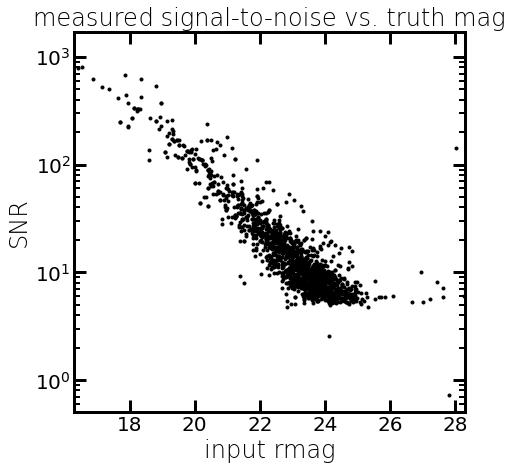
\includegraphics[width=3.12500in]{jira_imgs/3038.png}\\
We also demonstrate that the measurements agree with the ``true'' fluxes
of the simulated sources rather well:\\
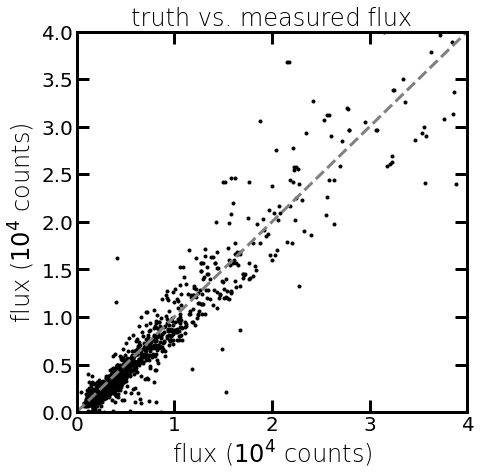
\includegraphics[width=3.12500in]{jira_imgs/3039.png}

}

\paragraph{ LVV-T131 - Verify implementation of Provide User Interface Services }\mbox{}\\

Version \textbf{1}.
Open  \href{https://jira.lsstcorp.org/secure/Tests.jspa#/testCase/LVV-T131}{\textit{ LVV-T131 } }
test case in Jira.

Verify the availability and functionality of the broad range of user
interface services called for in the requirement, as applied to both
Nightly and DRP data. ~This will primarily be done by verifications
performed at the LSST Science Platform level, based on the requirements
in \citeds{LDM-554}; however, a high-level set of tests corresponding to the
DMS-REQ-0160 requirement are defined below.

\textbf{ Preconditions}:\\
\begin{enumerate}
\tightlist
\item
  Testing this requirement relies on a set of data products meeting the
  data model implied by the DPDD existing in a deployment of the Science
  Platform and its underlying database and file services.

  \begin{enumerate}
  \tightlist
  \item
    In particular, both image and catalog data products are required.
  \item
    From the specific language of the underlying requirement, it appears
    clear that coadded data products are required, but in practice
    single-epoch data products should be included in the test as well.
  \end{enumerate}
\item
  Depending on when this requirement is tested, the tests may involve
  either or both of precursor data and LSST commissioning data. ~The use
  of the latter is ultimately essential to ensure that the tests are
  performed with as LSST-like a dataset as possible.
\end{enumerate}

Execution status: {\bf Not Executed }

Final comment:\\


Detailed steps results:

\begin{tabular}{p{2cm}p{14cm}}
\toprule
Step 1 & Step Execution Status: \textbf{ Not Executed } \\ \hline
\end{tabular}
 Description \\
{\footnotesize
\textbf{Establishment of test coordinates:}\\
Establish sky positions and surrounding regions (e.g., cones or
polygons), field sizes, filter bands, and temporal epochs for the tests
that are consistent with the known content of the test dataset, whether
precursor or LSST commissioning data.\\
Establishing sky positions should include pre-determining the
corresponding LSST ``tract and patch'' identifiers.\\
If the plan to not keep all calibrated single-epoch images on disk is
still in place at the time of the test, identify for use in the test
both images that are, and are not, on disk.\\
Establish target image boundaries, projections, and pixel scales to be
used for resampling tests. ~Ensure that at least some of these test
conditions include coadded image boundaries that cross tract and patch
boundaries, and single-epoch image boundaries that cross focal plane
raft boundaries.

}
\hdashrule[0.5ex]{\textwidth}{1pt}{3mm}
  Expected Result \\
{\footnotesize

}
\hdashrule[0.5ex]{\textwidth}{1pt}{3mm}
  Actual Result \\
{\footnotesize

}
\begin{tabular}{p{2cm}p{14cm}}
\toprule
Step 2 & Step Execution Status: \textbf{ Not Executed } \\ \hline
\end{tabular}
 Description \\
{\footnotesize
\textbf{Butler image access:}\\
From within the Notebook Aspect, verify that coadded images for the
identified regions of sky and filter bands are accessible via the
Butler. ~Verify that the same images are available whether obtained by
direct reference to the previous established tract/patch identifiers or
by the use of LSST stack code for retrieving images based on sky
coordinates.\\
From within the Notebook Aspect, verify that single-epoch raw images for
the selected locations and times are available. ~Verify that calibrated
images (PVIs) for the selected locations and times are available;
depending on the details of the test dataset, verify that PVIs still on
disk can be retrieved immediately.\\
Verify that lists or tables of image metadata, not just individual
images, can be retrieved. ~E.g., a list of all the single-epoch images
covering a selected sky location.

}
\hdashrule[0.5ex]{\textwidth}{1pt}{3mm}
  Expected Result \\
{\footnotesize

}
\hdashrule[0.5ex]{\textwidth}{1pt}{3mm}
  Actual Result \\
{\footnotesize

}
\begin{tabular}{p{2cm}p{14cm}}
\toprule
Step 3 & Step Execution Status: \textbf{ Not Executed } \\ \hline
\end{tabular}
 Description \\
{\footnotesize
\textbf{Programmatic PVI re-creation:}\\
From within the Notebook Aspect, verify that the recreation on demand of
a PVI can be performed. ~Ideally, this should be done as follows:

\begin{itemize}
\tightlist
\item
  Verify that recreation of a PVI that \emph{is} still available works
  and that it reproduces the original PVI exactly (except for provenance
  metadata that must be different) or within the reasonable ability of
  processing systems to do so (e.g., taking into account that the
  original calibration and the recreation may have run on different CPU
  architectures).
\item
  The test conditions should ensure the verification that a recreation
  was actually performed, i.e., that the still-available PVI was not
  returned instead.
\item
  Note that it does not appear to be a requirement that \emph{at Butler
  level} recreation on demand of PVIs is a completely transparent
  process. ~If this \emph{is} decided to be a requirement, the test must
  also verify that it has been satisfied. ~If it is \emph{not} a
  requirement, verify that adequate documentation on the PVI-recreation
  process (e.g., the SuperTasks and configuration to be used) is
  available.
\end{itemize}

}
\hdashrule[0.5ex]{\textwidth}{1pt}{3mm}
  Expected Result \\
{\footnotesize

}
\hdashrule[0.5ex]{\textwidth}{1pt}{3mm}
  Actual Result \\
{\footnotesize

}
\begin{tabular}{p{2cm}p{14cm}}
\toprule
Step 4 & Step Execution Status: \textbf{ Not Executed } \\ \hline
\end{tabular}
 Description \\
{\footnotesize
\textbf{Butler catalog access:}\\
From within the Notebook Aspect, verify that all the catalog data
products described in the DPDD can be retrieved for the coordinates
selected above via the Butler. (This test should include access to
SSObject data, but the details of how such a test would depend on the
coordinate selections require additional thought.)

}
\hdashrule[0.5ex]{\textwidth}{1pt}{3mm}
  Expected Result \\
{\footnotesize

}
\hdashrule[0.5ex]{\textwidth}{1pt}{3mm}
  Actual Result \\
{\footnotesize

}
\begin{tabular}{p{2cm}p{14cm}}
\toprule
Step 5 & Step Execution Status: \textbf{ Not Executed } \\ \hline
\end{tabular}
 Description \\
{\footnotesize
\textbf{LSST-stack-based resampling/reprojection:}\\
Verify the availability of software in the LSST stack, and associated
documentation, that permits the resampling of LSST images to different
pixel grids and projections.\\
Exercise this capability for the test conditions selected in Step 1
above.\\
Perform photometric and astrometric tests on the resulting resampled
images to provide evidence that the transformations performed were
correct to the accuracy supported by the data.

}
\hdashrule[0.5ex]{\textwidth}{1pt}{3mm}
  Expected Result \\
{\footnotesize

}
\hdashrule[0.5ex]{\textwidth}{1pt}{3mm}
  Actual Result \\
{\footnotesize

}
\begin{tabular}{p{2cm}p{14cm}}
\toprule
Step 6 & Step Execution Status: \textbf{ Not Executed } \\ \hline
\end{tabular}
 Description \\
{\footnotesize
\textbf{Comment:}\\
The following API Aspect test steps should be carried out on the
required ``offsite-like'' test platform, to ensure that their success
does not reflect any privileged access given to processes inside the
Data Access Center or other Science Platform instance. ~However, at
least a small sampling of them should \emph{also} be carried out
\emph{within} the Science Platform environment, i.e., in the Notebook
Aspect, and the results compared.

}
\hdashrule[0.5ex]{\textwidth}{1pt}{3mm}
  Expected Result \\
{\footnotesize

}
\hdashrule[0.5ex]{\textwidth}{1pt}{3mm}
  Actual Result \\
{\footnotesize

}
\begin{tabular}{p{2cm}p{14cm}}
\toprule
Step 7 & Step Execution Status: \textbf{ Not Executed } \\ \hline
\end{tabular}
 Description \\
{\footnotesize
\textbf{API Aspect image access:}\\
Using IVOA services such as the Registry and ObsTAP, from the
``offsite-like'' test platform, verify that the existence of the classes
of image data products foreseen in the DPDD can be determined.\\
Verify that ObsTAP and/or SIAv2 can be used to find the same images and
lists of images for the established test coordinates that were retrieved
via the Butler in Step 2 above.\\
Verify that the selected images are retrievable from the Web services.\\
Verify that the retrieved images are identical in their pixel content
and metadata.\\
The tests must include both coadded and single-epoch images.

}
\hdashrule[0.5ex]{\textwidth}{1pt}{3mm}
  Expected Result \\
{\footnotesize

}
\hdashrule[0.5ex]{\textwidth}{1pt}{3mm}
  Actual Result \\
{\footnotesize

}
\begin{tabular}{p{2cm}p{14cm}}
\toprule
Step 8 & Step Execution Status: \textbf{ Not Executed } \\ \hline
\end{tabular}
 Description \\
{\footnotesize
\textbf{API Aspect image transformations:}\\
Verify that image cutouts and resamplings can be performed via the IVOA
SODA service, and that the results are identical to those obtained for
the same parameters from the LSST-stack-based tests in Step 5.\\
(The requirements for supported reprojections, if any, in the SODA
service have not been established at the time of writing.)

}
\hdashrule[0.5ex]{\textwidth}{1pt}{3mm}
  Expected Result \\
{\footnotesize

}
\hdashrule[0.5ex]{\textwidth}{1pt}{3mm}
  Actual Result \\
{\footnotesize

}
\begin{tabular}{p{2cm}p{14cm}}
\toprule
Step 9 & Step Execution Status: \textbf{ Not Executed } \\ \hline
\end{tabular}
 Description \\
{\footnotesize
\textbf{API Aspect catalog data access:}\\
Verify that the IVOA Registry, RegTAP, TAP\_SCHEMA, and other relevant
mechanisms can be used to discover the existence of all the catalog data
products foreseen in the DPDD.\\
Using the IVOA TAP service, verify that all the catalog data products
foreseen in the DPDD can be retrieved for the coordinates determined in
Step 1. ~Verify that their scientific content is the same as when they
are retrieved via the Butler.

}
\hdashrule[0.5ex]{\textwidth}{1pt}{3mm}
  Expected Result \\
{\footnotesize

}
\hdashrule[0.5ex]{\textwidth}{1pt}{3mm}
  Actual Result \\
{\footnotesize

}
\begin{tabular}{p{2cm}p{14cm}}
\toprule
Step 10 & Step Execution Status: \textbf{ Not Executed } \\ \hline
\end{tabular}
 Description \\
{\footnotesize
\textbf{Comment:}\\
The Portal Aspect tests below should be carried out from a web browser
on an ``offsite-like'' test platform, to ensure that no privileged
access provided to intra-data-center clients is relied upon.

}
\hdashrule[0.5ex]{\textwidth}{1pt}{3mm}
  Expected Result \\
{\footnotesize

}
\hdashrule[0.5ex]{\textwidth}{1pt}{3mm}
  Actual Result \\
{\footnotesize

}
\begin{tabular}{p{2cm}p{14cm}}
\toprule
Step 11 & Step Execution Status: \textbf{ Not Executed } \\ \hline
\end{tabular}
 Description \\
{\footnotesize
\textbf{Portal Aspect data browsing:}\\
Verify that the Portal Aspect can be used to discover the existence of
all the data products foreseen in the DPDD. ~Verify that the UI permits
locating the data for the coordinates selected in Step 1 by visual
means, e.g., by zooming and panning in from an all-sky view.\\
Verify that the UI permits locating the data by typing in coordinates as
well.

}
\hdashrule[0.5ex]{\textwidth}{1pt}{3mm}
  Expected Result \\
{\footnotesize

}
\hdashrule[0.5ex]{\textwidth}{1pt}{3mm}
  Actual Result \\
{\footnotesize

}
\begin{tabular}{p{2cm}p{14cm}}
\toprule
Step 12 & Step Execution Status: \textbf{ Not Executed } \\ \hline
\end{tabular}
 Description \\
{\footnotesize
\textbf{Portal Aspect image access:}\\
Verify that the Portal Aspect allows both the retrieval of ``original''
image data, i.e., in its native LSST pixel projection and with full
metadata, as well as retrieval of on-demand UI cutouts of coadded image
data for selected locations.

}
\hdashrule[0.5ex]{\textwidth}{1pt}{3mm}
  Expected Result \\
{\footnotesize

}
\hdashrule[0.5ex]{\textwidth}{1pt}{3mm}
  Actual Result \\
{\footnotesize

}
\begin{tabular}{p{2cm}p{14cm}}
\toprule
Step 13 & Step Execution Status: \textbf{ Not Executed } \\ \hline
\end{tabular}
 Description \\
{\footnotesize
\textbf{Portal Aspect catalog query and visualization:}\\
Verify that the Portal Aspect allows graphical querying of DPDD catalog
data, both coadded and single-epoch, for selected regions of sky and/or
with selected properties, and supports the visualization of the results
(including histogramming, scatterplots, time series, table
manipulations, and overplotting on image data).\\
(Note that the Science Platform requirements, LDM-554, lay out a
detailed set of requirements on the selection and visualization of
catalog data.)

}
\hdashrule[0.5ex]{\textwidth}{1pt}{3mm}
  Expected Result \\
{\footnotesize

}
\hdashrule[0.5ex]{\textwidth}{1pt}{3mm}
  Actual Result \\
{\footnotesize

}
\begin{tabular}{p{2cm}p{14cm}}
\toprule
Step 14 & Step Execution Status: \textbf{ Not Executed } \\ \hline
\end{tabular}
 Description \\
{\footnotesize
\textbf{Portal Aspect data download:}\\
Verify that data identified and/or visualized in the Portal Aspect can
be downloaded to the remote system running the web browser in which the
Portal is displayed, as well as to the User Workspace.

}
\hdashrule[0.5ex]{\textwidth}{1pt}{3mm}
  Expected Result \\
{\footnotesize

}
\hdashrule[0.5ex]{\textwidth}{1pt}{3mm}
  Actual Result \\
{\footnotesize

}

\paragraph{ LVV-T79 - Verify implementation of PSF-Matched Coadds }\mbox{}\\

Version \textbf{1}.
Open  \href{https://jira.lsstcorp.org/secure/Tests.jspa#/testCase/LVV-T79}{\textit{ LVV-T79 } }
test case in Jira.

Verify that the DRP pipelines produce PSF matched coadds.

\textbf{ Preconditions}:\\


Execution status: {\bf Not Executed }

Final comment:\\


Detailed steps results:

\begin{tabular}{p{2cm}p{14cm}}
\toprule
Step 1 & Step Execution Status: \textbf{ Not Executed } \\ \hline
\end{tabular}
 Description \\
{\footnotesize
Identify the path to the data repository, which we will refer to as
`DATA/path', then execute the following:

}
\hdashrule[0.5ex]{\textwidth}{1pt}{3mm}
  Example Code \\
{\footnotesize
\begin{verbatim}
from lsst.daf.butler import Butler
repo = 'Data/path'
collection = 'collection'
butler = Butler(repo, collections=collection)
\end{verbatim}

}
\hdashrule[0.5ex]{\textwidth}{1pt}{3mm}
  Expected Result \\
{\footnotesize
Butler repo available for reading.

}
\hdashrule[0.5ex]{\textwidth}{1pt}{3mm}
  Actual Result \\
{\footnotesize

}
\begin{tabular}{p{2cm}p{14cm}}
\toprule
Step 2 & Step Execution Status: \textbf{ Not Executed } \\ \hline
\end{tabular}
 Description \\
{\footnotesize
Verify that PSF-matched coadds were created.

}
\hdashrule[0.5ex]{\textwidth}{1pt}{3mm}
  Expected Result \\
{\footnotesize

}
\hdashrule[0.5ex]{\textwidth}{1pt}{3mm}
  Actual Result \\
{\footnotesize

}

\paragraph{ LVV-T1830 - Verify Implementation of Scientific Visualization of Camera Image Data }\mbox{}\\

Version \textbf{1}.
Open  \href{https://jira.lsstcorp.org/secure/Tests.jspa#/testCase/LVV-T1830}{\textit{ LVV-T1830 } }
test case in Jira.

Verify that all scientific visualization of camera image data uses the
coordinate systems defined in \href{https://lse-349.lsst.io/}{LSE-349}.

\textbf{ Preconditions}:\\


Execution status: {\bf Not Executed }

Final comment:\\


Detailed steps results:

\begin{tabular}{p{2cm}p{14cm}}
\toprule
Step 1 & Step Execution Status: \textbf{ Not Executed } \\ \hline
\end{tabular}
 Description \\
{\footnotesize
Identify an image containing bright saturated stars. Load this image
into an image viewer such as Firefly or DS9.

}
\hdashrule[0.5ex]{\textwidth}{1pt}{3mm}
  Expected Result \\
{\footnotesize
Image with bright stars is displayed.

}
\hdashrule[0.5ex]{\textwidth}{1pt}{3mm}
  Actual Result \\
{\footnotesize

}
\begin{tabular}{p{2cm}p{14cm}}
\toprule
Step 2 & Step Execution Status: \textbf{ Not Executed } \\ \hline
\end{tabular}
 Description \\
{\footnotesize
Confirm that each of the following is true:\\

\begin{itemize}
\tightlist
\item
  the XY coordinate origin is at the lower left,
\item
  the x-coordinate increases left-to-right, and the y-coordinate
  increases bottom-to-top
\item
  bleed trails of saturated stars are vertical (i.e., the parallel
  transfer direction is oriented vertically)
\item
  the sky orientation places east 90 degrees counter-clockwise from
  north
\end{itemize}

}
\hdashrule[0.5ex]{\textwidth}{1pt}{3mm}
  Expected Result \\
{\footnotesize
Via coordinate grid overlays or similar, an image is demonstrated to
meet the necessary conditions.

}
\hdashrule[0.5ex]{\textwidth}{1pt}{3mm}
  Actual Result \\
{\footnotesize

}

\paragraph{ LVV-T98 - Verify implementation of Selection of Datasets }\mbox{}\\

Version \textbf{1}.
Open  \href{https://jira.lsstcorp.org/secure/Tests.jspa#/testCase/LVV-T98}{\textit{ LVV-T98 } }
test case in Jira.

Verify that the DMS can identify and retrieve datasets consisting of
logical groupings of Exposures, metadata, provenance, etc., or other
groupings that are processed or produced as a logical unit.

\textbf{ Preconditions}:\\


Execution status: {\bf Not Executed }

Final comment:\\


Detailed steps results:

\begin{tabular}{p{2cm}p{14cm}}
\toprule
Step 1 & Step Execution Status: \textbf{ Not Executed } \\ \hline
\end{tabular}
 Description \\
{\footnotesize
Identify the path to the data repository, which we will refer to as
`DATA/path', then execute the following:

}
\hdashrule[0.5ex]{\textwidth}{1pt}{3mm}
  Example Code \\
{\footnotesize
\begin{verbatim}
from lsst.daf.butler import Butler
repo = 'Data/path'
collection = 'collection'
butler = Butler(repo, collections=collection)
\end{verbatim}

}
\hdashrule[0.5ex]{\textwidth}{1pt}{3mm}
  Expected Result \\
{\footnotesize
Butler repo available for reading.

}
\hdashrule[0.5ex]{\textwidth}{1pt}{3mm}
  Actual Result \\
{\footnotesize

}
\begin{tabular}{p{2cm}p{14cm}}
\toprule
Step 2 & Step Execution Status: \textbf{ Not Executed } \\ \hline
\end{tabular}
 Description \\
{\footnotesize
Ingest data from an appropriate processed dataset.

}
\hdashrule[0.5ex]{\textwidth}{1pt}{3mm}
  Expected Result \\
{\footnotesize

}
\hdashrule[0.5ex]{\textwidth}{1pt}{3mm}
  Actual Result \\
{\footnotesize

}
\begin{tabular}{p{2cm}p{14cm}}
\toprule
Step 3 & Step Execution Status: \textbf{ Not Executed } \\ \hline
\end{tabular}
 Description \\
{\footnotesize
Observe retrieval of single Processed Visit Image (PVI) with metadata.

}
\hdashrule[0.5ex]{\textwidth}{1pt}{3mm}
  Expected Result \\
{\footnotesize
A PVI and its associated metadata.

}
\hdashrule[0.5ex]{\textwidth}{1pt}{3mm}
  Actual Result \\
{\footnotesize

}
\begin{tabular}{p{2cm}p{14cm}}
\toprule
Step 4 & Step Execution Status: \textbf{ Not Executed } \\ \hline
\end{tabular}
 Description \\
{\footnotesize
Observe retrieval of multiple PVIs with metadata.

}
\hdashrule[0.5ex]{\textwidth}{1pt}{3mm}
  Expected Result \\
{\footnotesize
A set of PVIs and their associated metadata.

}
\hdashrule[0.5ex]{\textwidth}{1pt}{3mm}
  Actual Result \\
{\footnotesize

}
\begin{tabular}{p{2cm}p{14cm}}
\toprule
Step 5 & Step Execution Status: \textbf{ Not Executed } \\ \hline
\end{tabular}
 Description \\
{\footnotesize
Observe retrieval of coadd patch with metadata and provenance
information.

}
\hdashrule[0.5ex]{\textwidth}{1pt}{3mm}
  Expected Result \\
{\footnotesize
An image of coadded data in a patch, along with its metadata and
information describing the provenance of the patch constituents.

}
\hdashrule[0.5ex]{\textwidth}{1pt}{3mm}
  Actual Result \\
{\footnotesize

}
\begin{tabular}{p{2cm}p{14cm}}
\toprule
Step 6 & Step Execution Status: \textbf{ Not Executed } \\ \hline
\end{tabular}
 Description \\
{\footnotesize
Observe retrieval of subset of rows in each of the above catalogs.

}
\hdashrule[0.5ex]{\textwidth}{1pt}{3mm}
  Expected Result \\
{\footnotesize

}
\hdashrule[0.5ex]{\textwidth}{1pt}{3mm}
  Actual Result \\
{\footnotesize

}

\paragraph{ LVV-T145 - Verify implementation of Task Configuration }\mbox{}\\

Version \textbf{1}.
Open  \href{https://jira.lsstcorp.org/secure/Tests.jspa#/testCase/LVV-T145}{\textit{ LVV-T145 } }
test case in Jira.

Verify that the DMS software provides configuration control to define,
override, and verify the configuration for a DMS Task.

\textbf{ Preconditions}:\\


Execution status: {\bf Not Executed }

Final comment:\\


Detailed steps results:

\begin{tabular}{p{2cm}p{14cm}}
\toprule
Step 1 & Step Execution Status: \textbf{ Not Executed } \\ \hline
\end{tabular}
 Description \\
{\footnotesize
Inspect software design to verify that one can define the configuration
for a Task.

}
\hdashrule[0.5ex]{\textwidth}{1pt}{3mm}
  Expected Result \\
{\footnotesize

}
\hdashrule[0.5ex]{\textwidth}{1pt}{3mm}
  Actual Result \\
{\footnotesize

}
\begin{tabular}{p{2cm}p{14cm}}
\toprule
Step 2 & Step Execution Status: \textbf{ Not Executed } \\ \hline
\end{tabular}
 Description \\
{\footnotesize
Run a Task with a known invalid configuration. ~Verify that the error is
caught before the science algorithm executes.

}
\hdashrule[0.5ex]{\textwidth}{1pt}{3mm}
  Expected Result \\
{\footnotesize

}
\hdashrule[0.5ex]{\textwidth}{1pt}{3mm}
  Actual Result \\
{\footnotesize

}
\begin{tabular}{p{2cm}p{14cm}}
\toprule
Step 3 & Step Execution Status: \textbf{ Not Executed } \\ \hline
\end{tabular}
 Description \\
{\footnotesize
Run a simple task with two different configurations that make a material
difference for a Task. ~E.g., specify a different source detection
threshold. ~Verify that the configuration is different between the two
runs through difference in recorded provenance and in results.

}
\hdashrule[0.5ex]{\textwidth}{1pt}{3mm}
  Expected Result \\
{\footnotesize

}
\hdashrule[0.5ex]{\textwidth}{1pt}{3mm}
  Actual Result \\
{\footnotesize

}

\paragraph{ LVV-T144 - Verify implementation of Task Specification }\mbox{}\\

Version \textbf{1}.
Open  \href{https://jira.lsstcorp.org/secure/Tests.jspa#/testCase/LVV-T144}{\textit{ LVV-T144 } }
test case in Jira.

Verify that the DMS provides the ability to define a new or modified
pipeline task without recompilation.

\textbf{ Preconditions}:\\


Execution status: {\bf Not Executed }

Final comment:\\


Detailed steps results:

\begin{tabular}{p{2cm}p{14cm}}
\toprule
Step 1 & Step Execution Status: \textbf{ Not Executed } \\ \hline
\end{tabular}
 Description \\
{\footnotesize
Inspect software architecture. ~Verify that there exist Tasks that can
be run and configured without re-compilation.

}
\hdashrule[0.5ex]{\textwidth}{1pt}{3mm}
  Expected Result \\
{\footnotesize
Confirmation that the software architecture has allowed for
reconfiguring and running Tasks without recompilation.

}
\hdashrule[0.5ex]{\textwidth}{1pt}{3mm}
  Actual Result \\
{\footnotesize

}
\begin{tabular}{p{2cm}p{14cm}}
\toprule
Step 2 & Step Execution Status: \textbf{ Not Executed } \\ \hline
\end{tabular}
 Description \\
{\footnotesize
Verify that an example science algorithm can be run through one of these
Tasks.~ Three examples from different areas: source measurement, image
subtraction, and photometric-redshift estimation.

}
\hdashrule[0.5ex]{\textwidth}{1pt}{3mm}
  Expected Result \\
{\footnotesize
Successful Task execution with different configurations, including
confirmation that the outputs are different from tasks with altered
configurations.

}
\hdashrule[0.5ex]{\textwidth}{1pt}{3mm}
  Actual Result \\
{\footnotesize

}

\paragraph{ LVV-T74 - Verify implementation of Template Coadds }\mbox{}\\

Version \textbf{1}.
Open  \href{https://jira.lsstcorp.org/secure/Tests.jspa#/testCase/LVV-T74}{\textit{ LVV-T74 } }
test case in Jira.

Verify that the DMS can produce Template Coadds for DIA processing.

\textbf{ Preconditions}:\\


Execution status: {\bf Pass }

Final comment:\\See attached artifact notebook ``test\_LVV-T74.ipynb'' for details.


Detailed steps results:

\begin{tabular}{p{2cm}p{14cm}}
\toprule
Step 1 & Step Execution Status: \textbf{ Pass } \\ \hline
\end{tabular}
 Description \\
{\footnotesize
Perform the steps of Alert Production (including, but not necessarily
limited to, single frame processing, ISR, source detection/measurement,
PSF estimation, photometric and astrometric calibration, difference
imaging, DIASource detection/measurement, source association). During
Operations, it is presumed that these are automated for a given
dataset.~

}
\hdashrule[0.5ex]{\textwidth}{1pt}{3mm}
  Expected Result \\
{\footnotesize
An output dataset including difference images and DIASource and
DIAObject measurements.

}
\hdashrule[0.5ex]{\textwidth}{1pt}{3mm}
  Actual Result \\
{\footnotesize
Logged into the RSP at the Interim Data Facility, and accessed the
shared butler repositories containing Data Preview 0.2 data. All work
for this Test Case is in Jupyter notebook ``test\_LVV-T74.ipynb'', which
is archived along with the test report.

}
\begin{tabular}{p{2cm}p{14cm}}
\toprule
Step 2 & Step Execution Status: \textbf{ Pass } \\ \hline
\end{tabular}
 Description \\
{\footnotesize
Verify that the expected data products have been produced, and that
catalogs contain reasonable values for measured quantities of interest.

}
\hdashrule[0.5ex]{\textwidth}{1pt}{3mm}
  Expected Result \\
{\footnotesize

}
\hdashrule[0.5ex]{\textwidth}{1pt}{3mm}
  Actual Result \\
{\footnotesize
We confirmed that the expected data products are present, including
DIASource tables, DIAObject measurements and their associations with
DIASource, template images, and that all have been photometrically and
astrometrically calibrated.

}
\begin{tabular}{p{2cm}p{14cm}}
\toprule
Step 3 & Step Execution Status: \textbf{ Pass } \\ \hline
\end{tabular}
 Description \\
{\footnotesize
Confirm that the template coadds have been created and are well-formed.

}
\hdashrule[0.5ex]{\textwidth}{1pt}{3mm}
  Expected Result \\
{\footnotesize

}
\hdashrule[0.5ex]{\textwidth}{1pt}{3mm}
  Actual Result \\
{\footnotesize
Finally, we displayed a template coadd and compared it to the original
image. See notebook ``test\_LVV-T74.ipynb'' for details.

}

\paragraph{ LVV-T97 - Verify implementation of Uniqueness of IDs Across Data Releases }\mbox{}\\

Version \textbf{1}.
Open  \href{https://jira.lsstcorp.org/secure/Tests.jspa#/testCase/LVV-T97}{\textit{ LVV-T97 } }
test case in Jira.

Verify that the IDs of Objects, Sources, DIAObjects, and DIASources from
different Data Releases are unique.

\textbf{ Preconditions}:\\


Execution status: {\bf Not Executed }

Final comment:\\


Detailed steps results:

\begin{tabular}{p{2cm}p{14cm}}
\toprule
Step 1 & Step Execution Status: \textbf{ Not Executed } \\ \hline
\end{tabular}
 Description \\
{\footnotesize
Identify an appropriate precursor dataset to be processed through Data
Release Production.

}
\hdashrule[0.5ex]{\textwidth}{1pt}{3mm}
  Expected Result \\
{\footnotesize

}
\hdashrule[0.5ex]{\textwidth}{1pt}{3mm}
  Actual Result \\
{\footnotesize

}
\begin{tabular}{p{2cm}p{14cm}}
\toprule
Step 2 & Step Execution Status: \textbf{ Not Executed } \\ \hline
\end{tabular}
 Description \\
{\footnotesize
Process data with the Data Release Production payload, starting from raw
science images and generating science data products, placing them in the
Data Backbone.

}
\hdashrule[0.5ex]{\textwidth}{1pt}{3mm}
  Expected Result \\
{\footnotesize

}
\hdashrule[0.5ex]{\textwidth}{1pt}{3mm}
  Actual Result \\
{\footnotesize

}
\begin{tabular}{p{2cm}p{14cm}}
\toprule
Step 3 & Step Execution Status: \textbf{ Not Executed } \\ \hline
\end{tabular}
 Description \\
{\footnotesize
Identify the path to the data repository, which we will refer to as
`DATA/path', then execute the following:

}
\hdashrule[0.5ex]{\textwidth}{1pt}{3mm}
  Example Code \\
{\footnotesize
\begin{verbatim}
from lsst.daf.butler import Butler
repo = 'Data/path'
collection = 'collection'
butler = Butler(repo, collections=collection)
\end{verbatim}

}
\hdashrule[0.5ex]{\textwidth}{1pt}{3mm}
  Expected Result \\
{\footnotesize
Butler repo available for reading.

}
\hdashrule[0.5ex]{\textwidth}{1pt}{3mm}
  Actual Result \\
{\footnotesize

}
\begin{tabular}{p{2cm}p{14cm}}
\toprule
Step 4 & Step Execution Status: \textbf{ Not Executed } \\ \hline
\end{tabular}
 Description \\
{\footnotesize
After running the DRP payload multiple times, load the resulting data
products (both data release and prompt products) using the Butler.

}
\hdashrule[0.5ex]{\textwidth}{1pt}{3mm}
  Expected Result \\
{\footnotesize
Multiple datasets resulting from processing of the same input data.

}
\hdashrule[0.5ex]{\textwidth}{1pt}{3mm}
  Actual Result \\
{\footnotesize

}
\begin{tabular}{p{2cm}p{14cm}}
\toprule
Step 5 & Step Execution Status: \textbf{ Not Executed } \\ \hline
\end{tabular}
 Description \\
{\footnotesize
Inspect the IDs in the multiple data products and confirm that all IDs
are unique.

}
\hdashrule[0.5ex]{\textwidth}{1pt}{3mm}
  Expected Result \\
{\footnotesize
No IDs are repeated between multiple processings of the identical input
dataset.

}
\hdashrule[0.5ex]{\textwidth}{1pt}{3mm}
  Actual Result \\
{\footnotesize

}

\paragraph{ LVV-T1529 - Verify Production of All-Sky HiPS Map }\mbox{}\\

Version \textbf{1}.
Open  \href{https://jira.lsstcorp.org/secure/Tests.jspa#/testCase/LVV-T1529}{\textit{ LVV-T1529 } }
test case in Jira.

Verify that Data Release Production includes the production of an
all-sky image map for the existing coadded image area in each filter
band, and at least one pre-defined all-sky color image map, following
the IVOA HiPS Recommendation.

\textbf{ Preconditions}:\\


Execution status: {\bf Not Executed }

Final comment:\\


Detailed steps results:

\begin{tabular}{p{2cm}p{14cm}}
\toprule
Step 1 & Step Execution Status: \textbf{ Not Executed } \\ \hline
\end{tabular}
 Description \\
{\footnotesize

}
\hdashrule[0.5ex]{\textwidth}{1pt}{3mm}
  Expected Result \\
{\footnotesize

}
\hdashrule[0.5ex]{\textwidth}{1pt}{3mm}
  Actual Result \\
{\footnotesize

}

\paragraph{ LVV-T1527 - Verify Support for HiPS Visualization }\mbox{}\\

Version \textbf{1}.
Open  \href{https://jira.lsstcorp.org/secure/Tests.jspa#/testCase/LVV-T1527}{\textit{ LVV-T1527 } }
test case in Jira.

Verify that the LSST Science Platform supports the visualization of
LSST-generated HiPS image maps as well as other HiPS maps which satisfy
the IVOA HiPS Recommendation. Also verify that integrated behavior is
available, such as the overplotting of catalog entries, comparable to
that provided for individual source images (e.g., PVIs and coadd tiles).

\textbf{ Preconditions}:\\


Execution status: {\bf Not Executed }

Final comment:\\


Detailed steps results:

\begin{tabular}{p{2cm}p{14cm}}
\toprule
Step 1 & Step Execution Status: \textbf{ Not Executed } \\ \hline
\end{tabular}
 Description \\
{\footnotesize

}
\hdashrule[0.5ex]{\textwidth}{1pt}{3mm}
  Expected Result \\
{\footnotesize

}
\hdashrule[0.5ex]{\textwidth}{1pt}{3mm}
  Actual Result \\
{\footnotesize

}

\paragraph{ LVV-T1758 - Verify that the repeatability outlier limit for isolated bright
non-saturated point sources in the u, z, and y filters (PA2uzy) can be
applied. }\mbox{}\\

Version \textbf{1}.
Open  \href{https://jira.lsstcorp.org/secure/Tests.jspa#/testCase/LVV-T1758}{\textit{ LVV-T1758 } }
test case in Jira.

Verify that the DM system has provided the code to apply the
repeatability outlier limit for isolated bright non-saturated point
sources in the u, z, and y filters(PA2uzy) to to computed values of the
PF1 metric.

\textbf{ Preconditions}:\\


Execution status: {\bf Not Executed }

Final comment:\\


Detailed steps results:

\begin{tabular}{p{2cm}p{14cm}}
\toprule
Step 1 & Step Execution Status: \textbf{ Not Executed } \\ \hline
\end{tabular}
 Description \\
{\footnotesize
Identify a dataset containing at least one field in each of the u, z,
and y filters with multiple overlapping visits.

}
\hdashrule[0.5ex]{\textwidth}{1pt}{3mm}
  Expected Result \\
{\footnotesize
A dataset that has been ingested into a Butler repository.

}
\hdashrule[0.5ex]{\textwidth}{1pt}{3mm}
  Actual Result \\
{\footnotesize

}
\begin{tabular}{p{2cm}p{14cm}}
\toprule
Step 2 & Step Execution Status: \textbf{ Not Executed } \\ \hline
\end{tabular}
 Description \\
{\footnotesize
The `path` that you will use depends on where you are running the
science pipelines. Options:\\[2\baselineskip]

\begin{itemize}
\tightlist
\item
  local (newinstall.sh - based
  install):{[}path\_to\_installation{]}/loadLSST.bash
\item
  development cluster (``lsst-dev''):
  /software/lsstsw/stack/loadLSST.bash
\item
  LSP Notebook aspect (from a terminal):
  /opt/lsst/software/stack/loadLSST.bash
\end{itemize}

From the command line, execute the commands below in the example
code:\\[2\baselineskip]

}
\hdashrule[0.5ex]{\textwidth}{1pt}{3mm}
  Example Code \\
{\footnotesize
source `path`\\
setup lsst\_distrib

}
\hdashrule[0.5ex]{\textwidth}{1pt}{3mm}
  Expected Result \\
{\footnotesize
Science pipeline software is available for use. If additional packages
are needed (for example, `obs' packages such as `obs\_subaru`), then
additional `setup` commands will be necessary.\\[2\baselineskip]To check
versions in use, type:\\
eups list -s

}
\hdashrule[0.5ex]{\textwidth}{1pt}{3mm}
  Actual Result \\
{\footnotesize

}
\begin{tabular}{p{2cm}p{14cm}}
\toprule
Step 3 & Step Execution Status: \textbf{ Not Executed } \\ \hline
\end{tabular}
 Description \\
{\footnotesize
Execute `faro` on a repository containing processed data. Identify the
path to the data, which we will call `DATA/path', then execute something
similar to the following (with paths, datasets, and flags replaced or
additionally specified as needed):

}
\hdashrule[0.5ex]{\textwidth}{1pt}{3mm}
  Example Code \\
{\footnotesize
pipetask --long-log run -j 2 -b DATA/path/butler.yaml
--register-dataset-types -p \$FARO\_DIR/pipelines/metrics\_pipeline.yaml
-d ``band in ('g', `r', `i') AND tract=9813 AND skymap='hsc\_rings\_v1'
AND instrument='HSC''' --output u/username/faro\_metrics -i
HSC/runs/RC2/w\_2021\_06 2\textgreater{}\&1 \textbar{} tee
w06\_2021\_tract9813\_faro.txt

}
\hdashrule[0.5ex]{\textwidth}{1pt}{3mm}
  Expected Result \\
{\footnotesize
The output collection (in this case, ``u/username/faro\_metrics'')
containing metric measurements and any associated extras and metadata is
available via the butler.

}
\hdashrule[0.5ex]{\textwidth}{1pt}{3mm}
  Actual Result \\
{\footnotesize

}
\begin{tabular}{p{2cm}p{14cm}}
\toprule
Step 4 & Step Execution Status: \textbf{ Not Executed } \\ \hline
\end{tabular}
 Description \\
{\footnotesize
Confirm that the PA2uzy threshold has been applied to the assessment of
the computed values of PF1 for filters u,z,y.

}
\hdashrule[0.5ex]{\textwidth}{1pt}{3mm}
  Expected Result \\
{\footnotesize
A JSON file (and/or a report generated from that JSON file)
demonstrating that PA2uzy has been calculated (and that it used PF1).

}
\hdashrule[0.5ex]{\textwidth}{1pt}{3mm}
  Actual Result \\
{\footnotesize

}

\paragraph{ LVV-T1528 - Verify Visualization of MOCs via Science Platform }\mbox{}\\

Version \textbf{1}.
Open  \href{https://jira.lsstcorp.org/secure/Tests.jspa#/testCase/LVV-T1528}{\textit{ LVV-T1528 } }
test case in Jira.

Verify that the LSST Science Platform supports the visualization of the
LSST-generated MOCs as well as other MOCs which satisfy the IVOA MOC
Recommendation.

\textbf{ Preconditions}:\\


Execution status: {\bf Not Executed }

Final comment:\\


Detailed steps results:

\begin{tabular}{p{2cm}p{14cm}}
\toprule
Step 1 & Step Execution Status: \textbf{ Not Executed } \\ \hline
\end{tabular}
 Description \\
{\footnotesize

}
\hdashrule[0.5ex]{\textwidth}{1pt}{3mm}
  Expected Result \\
{\footnotesize

}
\hdashrule[0.5ex]{\textwidth}{1pt}{3mm}
  Actual Result \\
{\footnotesize

}




% This appendix is put in as part of the template. You may edit and add to it.
% It is not overwritten by Docsteady.

\newpage
\appendix
\section{Documentation}
The verification process is defined in \citeds{LSE-160}.
The use of Docsteady to format Jira information in various test and planing documents is
described in \citeds{DMTN-140} and practical commands are given in \citeds{DMTN-178}.

\section{Acronyms used in this document}\label{sec:acronyms}
\input{acronyms.tex}

\newpage

% Uncomment this if Docsteady makes you additional appendix
%\input{DMTR-371.appendix.tex}

\end{document}
